% Options for packages loaded elsewhere
\PassOptionsToPackage{unicode}{hyperref}
\PassOptionsToPackage{hyphens}{url}
\PassOptionsToPackage{dvipsnames,svgnames,x11names}{xcolor}
%
\documentclass[
  letterpaper,
  DIV=11,
  numbers=noendperiod]{scrartcl}

\usepackage{amsmath,amssymb}
\usepackage{iftex}
\ifPDFTeX
  \usepackage[T1]{fontenc}
  \usepackage[utf8]{inputenc}
  \usepackage{textcomp} % provide euro and other symbols
\else % if luatex or xetex
  \usepackage{unicode-math}
  \defaultfontfeatures{Scale=MatchLowercase}
  \defaultfontfeatures[\rmfamily]{Ligatures=TeX,Scale=1}
\fi
\usepackage{lmodern}
\ifPDFTeX\else  
    % xetex/luatex font selection
\fi
% Use upquote if available, for straight quotes in verbatim environments
\IfFileExists{upquote.sty}{\usepackage{upquote}}{}
\IfFileExists{microtype.sty}{% use microtype if available
  \usepackage[]{microtype}
  \UseMicrotypeSet[protrusion]{basicmath} % disable protrusion for tt fonts
}{}
\makeatletter
\@ifundefined{KOMAClassName}{% if non-KOMA class
  \IfFileExists{parskip.sty}{%
    \usepackage{parskip}
  }{% else
    \setlength{\parindent}{0pt}
    \setlength{\parskip}{6pt plus 2pt minus 1pt}}
}{% if KOMA class
  \KOMAoptions{parskip=half}}
\makeatother
\usepackage{xcolor}
\setlength{\emergencystretch}{3em} % prevent overfull lines
\setcounter{secnumdepth}{5}
% Make \paragraph and \subparagraph free-standing
\ifx\paragraph\undefined\else
  \let\oldparagraph\paragraph
  \renewcommand{\paragraph}[1]{\oldparagraph{#1}\mbox{}}
\fi
\ifx\subparagraph\undefined\else
  \let\oldsubparagraph\subparagraph
  \renewcommand{\subparagraph}[1]{\oldsubparagraph{#1}\mbox{}}
\fi


\providecommand{\tightlist}{%
  \setlength{\itemsep}{0pt}\setlength{\parskip}{0pt}}\usepackage{longtable,booktabs,array}
\usepackage{calc} % for calculating minipage widths
% Correct order of tables after \paragraph or \subparagraph
\usepackage{etoolbox}
\makeatletter
\patchcmd\longtable{\par}{\if@noskipsec\mbox{}\fi\par}{}{}
\makeatother
% Allow footnotes in longtable head/foot
\IfFileExists{footnotehyper.sty}{\usepackage{footnotehyper}}{\usepackage{footnote}}
\makesavenoteenv{longtable}
\usepackage{graphicx}
\makeatletter
\def\maxwidth{\ifdim\Gin@nat@width>\linewidth\linewidth\else\Gin@nat@width\fi}
\def\maxheight{\ifdim\Gin@nat@height>\textheight\textheight\else\Gin@nat@height\fi}
\makeatother
% Scale images if necessary, so that they will not overflow the page
% margins by default, and it is still possible to overwrite the defaults
% using explicit options in \includegraphics[width, height, ...]{}
\setkeys{Gin}{width=\maxwidth,height=\maxheight,keepaspectratio}
% Set default figure placement to htbp
\makeatletter
\def\fps@figure{htbp}
\makeatother
% definitions for citeproc citations
\NewDocumentCommand\citeproctext{}{}
\NewDocumentCommand\citeproc{mm}{%
  \begingroup\def\citeproctext{#2}\cite{#1}\endgroup}
\makeatletter
 % allow citations to break across lines
 \let\@cite@ofmt\@firstofone
 % avoid brackets around text for \cite:
 \def\@biblabel#1{}
 \def\@cite#1#2{{#1\if@tempswa , #2\fi}}
\makeatother
\newlength{\cslhangindent}
\setlength{\cslhangindent}{1.5em}
\newlength{\csllabelwidth}
\setlength{\csllabelwidth}{3em}
\newenvironment{CSLReferences}[2] % #1 hanging-indent, #2 entry-spacing
 {\begin{list}{}{%
  \setlength{\itemindent}{0pt}
  \setlength{\leftmargin}{0pt}
  \setlength{\parsep}{0pt}
  % turn on hanging indent if param 1 is 1
  \ifodd #1
   \setlength{\leftmargin}{\cslhangindent}
   \setlength{\itemindent}{-1\cslhangindent}
  \fi
  % set entry spacing
  \setlength{\itemsep}{#2\baselineskip}}}
 {\end{list}}
\usepackage{calc}
\newcommand{\CSLBlock}[1]{\hfill\break\parbox[t]{\linewidth}{\strut\ignorespaces#1\strut}}
\newcommand{\CSLLeftMargin}[1]{\parbox[t]{\csllabelwidth}{\strut#1\strut}}
\newcommand{\CSLRightInline}[1]{\parbox[t]{\linewidth - \csllabelwidth}{\strut#1\strut}}
\newcommand{\CSLIndent}[1]{\hspace{\cslhangindent}#1}

\usepackage{booktabs}
\usepackage{longtable}
\usepackage{array}
\usepackage{multirow}
\usepackage{wrapfig}
\usepackage{float}
\usepackage{colortbl}
\usepackage{pdflscape}
\usepackage{tabu}
\usepackage{threeparttable}
\usepackage{threeparttablex}
\usepackage[normalem]{ulem}
\usepackage{makecell}
\usepackage{xcolor}
\usepackage{tabularray}
\usepackage[normalem]{ulem}
\usepackage{graphicx}
\UseTblrLibrary{booktabs}
\UseTblrLibrary{rotating}
\UseTblrLibrary{siunitx}
\NewTableCommand{\tinytableDefineColor}[3]{\definecolor{#1}{#2}{#3}}
\newcommand{\tinytableTabularrayUnderline}[1]{\underline{#1}}
\newcommand{\tinytableTabularrayStrikeout}[1]{\sout{#1}}
\KOMAoption{captions}{tableheading}
\makeatletter
\@ifpackageloaded{caption}{}{\usepackage{caption}}
\AtBeginDocument{%
\ifdefined\contentsname
  \renewcommand*\contentsname{Table of contents}
\else
  \newcommand\contentsname{Table of contents}
\fi
\ifdefined\listfigurename
  \renewcommand*\listfigurename{List of Figures}
\else
  \newcommand\listfigurename{List of Figures}
\fi
\ifdefined\listtablename
  \renewcommand*\listtablename{List of Tables}
\else
  \newcommand\listtablename{List of Tables}
\fi
\ifdefined\figurename
  \renewcommand*\figurename{Figure}
\else
  \newcommand\figurename{Figure}
\fi
\ifdefined\tablename
  \renewcommand*\tablename{Table}
\else
  \newcommand\tablename{Table}
\fi
}
\@ifpackageloaded{float}{}{\usepackage{float}}
\floatstyle{ruled}
\@ifundefined{c@chapter}{\newfloat{codelisting}{h}{lop}}{\newfloat{codelisting}{h}{lop}[chapter]}
\floatname{codelisting}{Listing}
\newcommand*\listoflistings{\listof{codelisting}{List of Listings}}
\makeatother
\makeatletter
\makeatother
\makeatletter
\@ifpackageloaded{caption}{}{\usepackage{caption}}
\@ifpackageloaded{subcaption}{}{\usepackage{subcaption}}
\makeatother
\ifLuaTeX
  \usepackage{selnolig}  % disable illegal ligatures
\fi
\usepackage{bookmark}

\IfFileExists{xurl.sty}{\usepackage{xurl}}{} % add URL line breaks if available
\urlstyle{same} % disable monospaced font for URLs
\hypersetup{
  pdftitle={Demographic Factors and Climate Action: Understanding How Age and Education Shape Sustainable Choices},
  pdfauthor={Lexi Knight},
  colorlinks=true,
  linkcolor={blue},
  filecolor={Maroon},
  citecolor={Blue},
  urlcolor={Blue},
  pdfcreator={LaTeX via pandoc}}

\title{Demographic Factors and Climate Action: Understanding How Age and
Education Shape Sustainable Choices\thanks{Code and data are available
at: \url{https://github.com/LexiKnight/toronto_climate/tree/main}.}}
\usepackage{etoolbox}
\makeatletter
\providecommand{\subtitle}[1]{% add subtitle to \maketitle
  \apptocmd{\@title}{\par {\large #1 \par}}{}{}
}
\makeatother
\subtitle{Older Individuals and Those with Higher Education Show
Stronger Commitment to Long-Term Sustainable Actions}
\author{Lexi Knight}
\date{December 13, 2024}

\begin{document}
\maketitle
\begin{abstract}
This study investigates how age and education influence people's
likelihood to adopt climate-friendly behaviors, such as reducing car use
and conserving energy. The analysis shows that younger individuals and
those with higher education are more likely to engage in these actions,
while older people tend to focus on energy-saving behaviors. However,
financial barriers and doubts about the impact of individual actions
prevent many people from taking steps to address climate change. These
findings suggest that targeted policies are needed to make sustainable
choices more accessible to different groups, helping to drive broader
participation in climate action.
\end{abstract}

\renewcommand*\contentsname{Table of contents}
{
\hypersetup{linkcolor=}
\setcounter{tocdepth}{3}
\tableofcontents
}
\subsection{Introduction}\label{introduction}

Climate change is one of the most pressing issues of our time. Its
effects---rising temperatures, extreme weather events, and ecosystem
disruptions---are already being felt globally, and the urgency for
action has never been higher (Intergovernmental Panel on Climate Change
(IPCC) 2023). Despite widespread awareness of the risks associated with
climate change, many individuals still struggle to adopt behaviors that
could help mitigate its impact. This gap between understanding and
action is a major barrier to effective climate solutions, and
understanding the underlying reasons for this disconnect is essential
for crafting strategies that encourage widespread behavioral change
(Gifford 2011).

This paper seeks to explore how certain demographic
factors---specifically age and education---affect individuals'
likelihood to adopt climate-friendly behaviors. By analyzing data from a
2018 survey (City of Toronto 2024), we aim to understand how these
factors influence behaviors such as reducing energy consumption, using
greener transportation, and minimizing waste. The estimand of this study
is the effect of age and education on the likelihood of adopting these
climate-friendly behaviors. We focus on these variables to understand
whether younger, more educated individuals are more likely to engage in
sustainable actions, and whether targeted strategies could drive greater
participation in climate-positive behaviors.

Through our analysis, we found that younger individuals and those with
higher levels of education were more likely to adopt behaviors such as
reducing car usage and embracing plant-based diets (Fulton 2022).
However, older individuals were more inclined to engage in actions like
cutting down on household energy use (Lee 2019). This suggests that
while age and education are important predictors, the types of
climate-friendly behaviors people adopt may differ across these groups.
Additionally, we identified key barriers to adoption, including
financial cost and doubts about the effectiveness of individual actions,
which often prevent people from taking meaningful steps to reduce their
environmental impact (Kollmuss and Agyeman 2002). These insights
emphasize that a one-size-fits-all approach to climate communication and
action will not be effective; instead, strategies must be tailored to
address the specific needs and motivations of different demographic
groups.

The findings from this study are significant because they provide a
clearer understanding of how demographic characteristics shape the
adoption of climate-friendly behaviors. By identifying which groups are
more likely to act and which face greater barriers, we can design more
effective policies and interventions that speak directly to the concerns
of these populations. This study not only contributes to the broader
understanding of climate change engagement but also offers practical
insights for shaping messages and policies that can inspire individuals
to take action.

The remainder of this paper is structured as follows:
Section~\ref{sec-data} describes the data and methodology used for
analysis, Section~\ref{sec-model} outlines the statistical model used to
assess the effects of age and education on behavior adoption,
Section~\ref{sec-results} presents the key findings, and
Section~\ref{sec-discussion} explores the implications of these results,
addresses limitations, and suggests directions for future research.
Finally, Section~\ref{sec-conclusion} summarizes the main takeaways and
offers recommendations for enhancing climate action engagement.
Additional methodological details and the data cleaning process are
provided in Section~\ref{sec-appendix}.

\subsection{Data}\label{sec-data}

The primary data source for this project is the Climate Perception Study
dataset, provided by the City of Toronto via the Open Data Toronto
platform (City of Toronto 2024). This dataset offers insights into
public perceptions of climate change in Toronto in the years 2018 and
2021. This dataset was accessed from \texttt{Open\ Data\ Toronto}
({``Open Data Toronto''} 2024) on 6 November 2024.

\subsubsection{Software and R-packages}\label{software-and-r-packages}

This project was conducted using the statistical software \texttt{R} (R
Core Team 2023), with several packages facilitating data cleaning,
analysis and reporting. The \texttt{tidyverse} package (Wickham,
Averick, et al. 2024) was central to the project, with \texttt{dplyr}
(Wickham, François, et al. 2024) used in the cleaning and exploratory
data analysis scripts for filtering, summarizing, and joining datasets.
\texttt{readr} (Wickham, Hester, et al. 2024) handled reading and
writing text data, while \texttt{tidyr} (Wickham, Henry, et al. 2024)
reshaped data. \texttt{stringr} (Wickham 2024c) managed character
strings, and \texttt{forcats} (Wickham 2024a) reordered factor levels
for visualizations.

In the download script, \texttt{httr}(Wickham 2024b) retrieved files
from \texttt{Open\ Data\ Toronto} ({``Open Data Toronto''} 2024),
while\texttt{readxl} (Wickham and Bryan 2024) read Excel files, and
\texttt{openxlsx} (Walker et al. 2024) created structured Excel
workbooks. The \texttt{arrow} package (Richardson et al. 2024) optimized
data storage and was used in the simulation and cleaning scripts to save
datasets as Parquet files.

For modeling, \texttt{rpart} (Therneau and Atkinson 2024) and
\texttt{partykit} (Hothorn and Zeileis 2024) built and visualized
decision trees in the model script. The \texttt{testthat} package
(Wickham et al. 2024b) validated simulated and cleaned datasets in their
respective scripts. Visualizations were created using \texttt{ggplot2}
(Wickham et al. 2024a) in the exploratory data analysis. Reporting
relied on \texttt{knitr} (Xie 2024) and \texttt{kableExtra} (Zhu 2024)
to integrate code, outputs, and styled tables. The
\texttt{tinytable}package (Mikolas 2024) generated compact tables in
both the exploratory data analysis script as well as in the paper. These
packages ensured efficient and streamlined data management, analysis and
reporting throughout the project.

\subsubsection{Methodology}\label{methodology}

\paragraph{Data Collection}\label{data-collection}

To embark on this analysis, we turn to two pivotal surveys commissioned
by the City of Toronto to capture residents' perceptions of climate
change and their readiness to take action. Our journey begins in 2018,
when Environics Research conducted an online survey with 404 Toronto
residents aged 18 and older, from October 11 to 18. The sample, drawn
from an online panel, was carefully crafted with quotas based on region,
age, and gender to mirror the 2016 Census. A touch of minor weighting
ensured a more representative reflection of the population. However,
it's important to note that this non-random sample introduces some
potential bias, an aspect we keep in mind as we move forward.

The path continues in 2021 with Ipsos at the helm, stepping in with a
more expansive survey, engaging 1,400 residents from a mix of methods:
1,000 from an online panel, 300 via phone, and 100 through online
interviews conducted in Mandarin, Cantonese, and Punjabi. This diverse
approach sought to enhance the survey's representativeness across
Toronto's varied communities. For our analysis, we used Version 2 of the
2021 dataset, where responses were presented in a clear, numeric format,
offering a solid foundation for our exploration.

With this data in hand, we are now ready to delve into the intricacies
of the findings, unearthing patterns, and understanding the deeper story
they tell about Toronto's residents and their views on climate change
and collective action.

\paragraph{Data Analysis}\label{data-analysis}

The focus of this analysis was the 2018 dataset, which examined five key
variables: age, education, extent informed, likelihood to take action,
and preferred methods for delivering information about climate change
action. These variables were analyzed at the individual level, allowing
for an in-depth exploration of residents' perspectives.

For 2021, summary data was available instead of individual-level data.
To compare trends, I created summary data for 2018. Calculating the
percentage distribution for each variable in both years helped identify
shifts in demographics, public awareness, and engagement, as well as
changes in preferred communication methods. Although the absence of
individual data for 2021 posed a challenge, this comparison still
provided a dynamic view of evolving climate change perspectives in
Toronto. The two-step approach---detailing 2018 data and then comparing
it with 2021 trends---created a comprehensive narrative of change.

\subsubsection{Features}\label{features}

\paragraph{Age}\label{age}

\subparagraph{Individual 2018}\label{individual-2018}

Figure~\ref{fig-one} presents the age distribution of survey respondents
in 2018. The histogram shows the frequency of respondents across age
groups, with age intervals on the x-axis and the number of respondents
on the y-axis. The distribution is fairly balanced, with peaks around
the 30--40 and 50--60 age ranges, indicating that these groups were the
most represented in the survey.

The vertical dotted lines highlight the median and mean ages. The green
dotted line represents the median age, and the blue dashed line
represents the mean age, both located just above 45. This suggests the
sample is predominantly middle-aged, with a gradual decline in
respondent frequency after the age of 60. Few participants were over 80,
indicating a lower representation of older individuals

\begin{figure}

\centering{

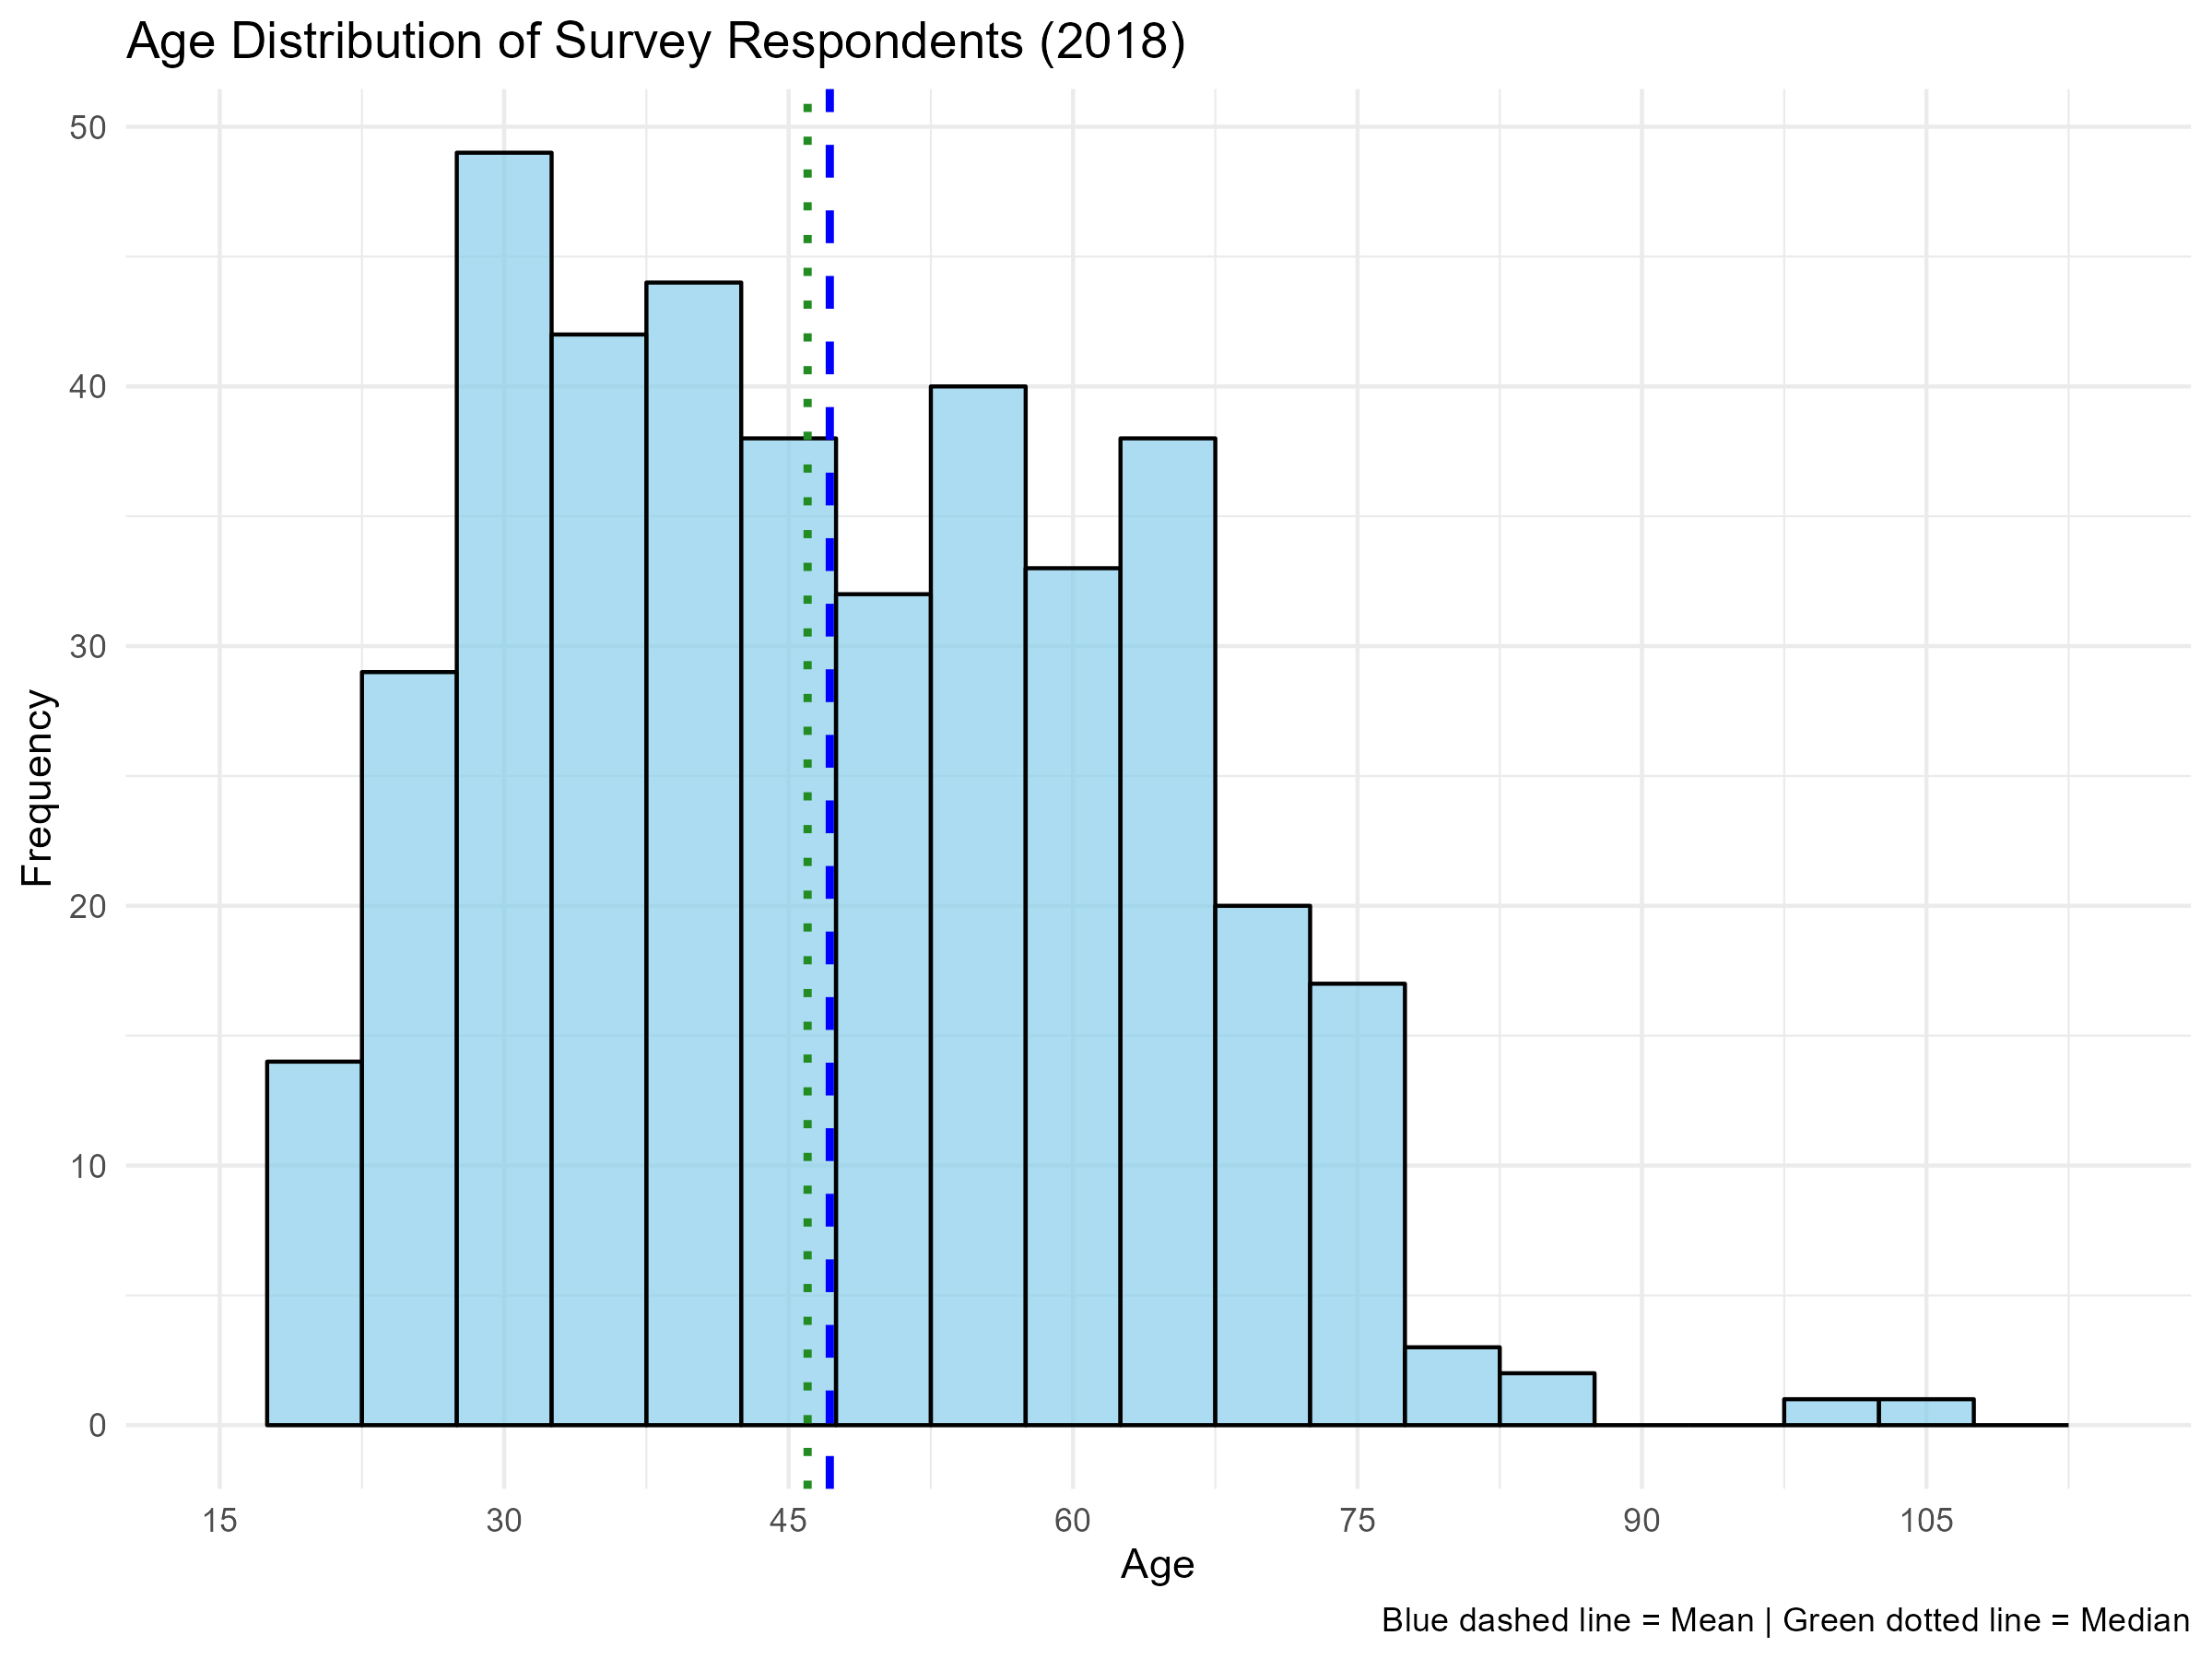
\includegraphics[width=6in,height=\textheight]{../data/03-figures_data/age_individual_plot.png}

}

\caption{\label{fig-one}Distribution of age given the 2018 survey
respondents. The mean and median of the sample is indicated with dashed
and dotted lines respectively.}

\end{figure}%

\newpage

\subparagraph{Comparison 2018 to 2021}\label{comparison-2018-to-2021}

Figure~\ref{fig-two} compares the age distributions between 2018 and
2021. The main difference is an increase in respondents aged 18-23 in
2021, with other age groups remaining relatively stable. This shift may
reflect changing demographic patterns or differences in survey
methodologies within the three years.

\begin{figure}

\centering{

\begin{table}
\centering
\begin{tabular}[t]{l|r|r}
\hline
Age Group & 2018 Percentage & 2021 Percentage\\
\hline
18-23 & 4 & 11\\
\hline
24-39 & 33 & 30\\
\hline
40-55 & 30 & 26\\
\hline
56+ & 33 & 33\\
\hline
\end{tabular}
\end{table}

}

\caption{\label{fig-two}This table highlights the age distribution of
survey respondents in 2018 and 2021.}

\end{figure}%

\paragraph{Education}\label{education}

\subparagraph{Individual 2018}\label{individual-2018-1}

Figure~\ref{fig-three} shows the distribution of respondents by their
highest level of education attained in 2018. The most common education
levels are ``Completed undergraduate degree'' and
``Postgraduate/professional school,'' indicating a well-educated
respondent population. In contrast, fewer respondents reported having
attended or completed community college, vocational, or trade school,
suggesting lower representation in these categories. A small portion of
respondents chose not to disclose their education level. Overall, the
distribution reflects a skew toward higher levels of educational
attainment.

\begin{figure}

\centering{

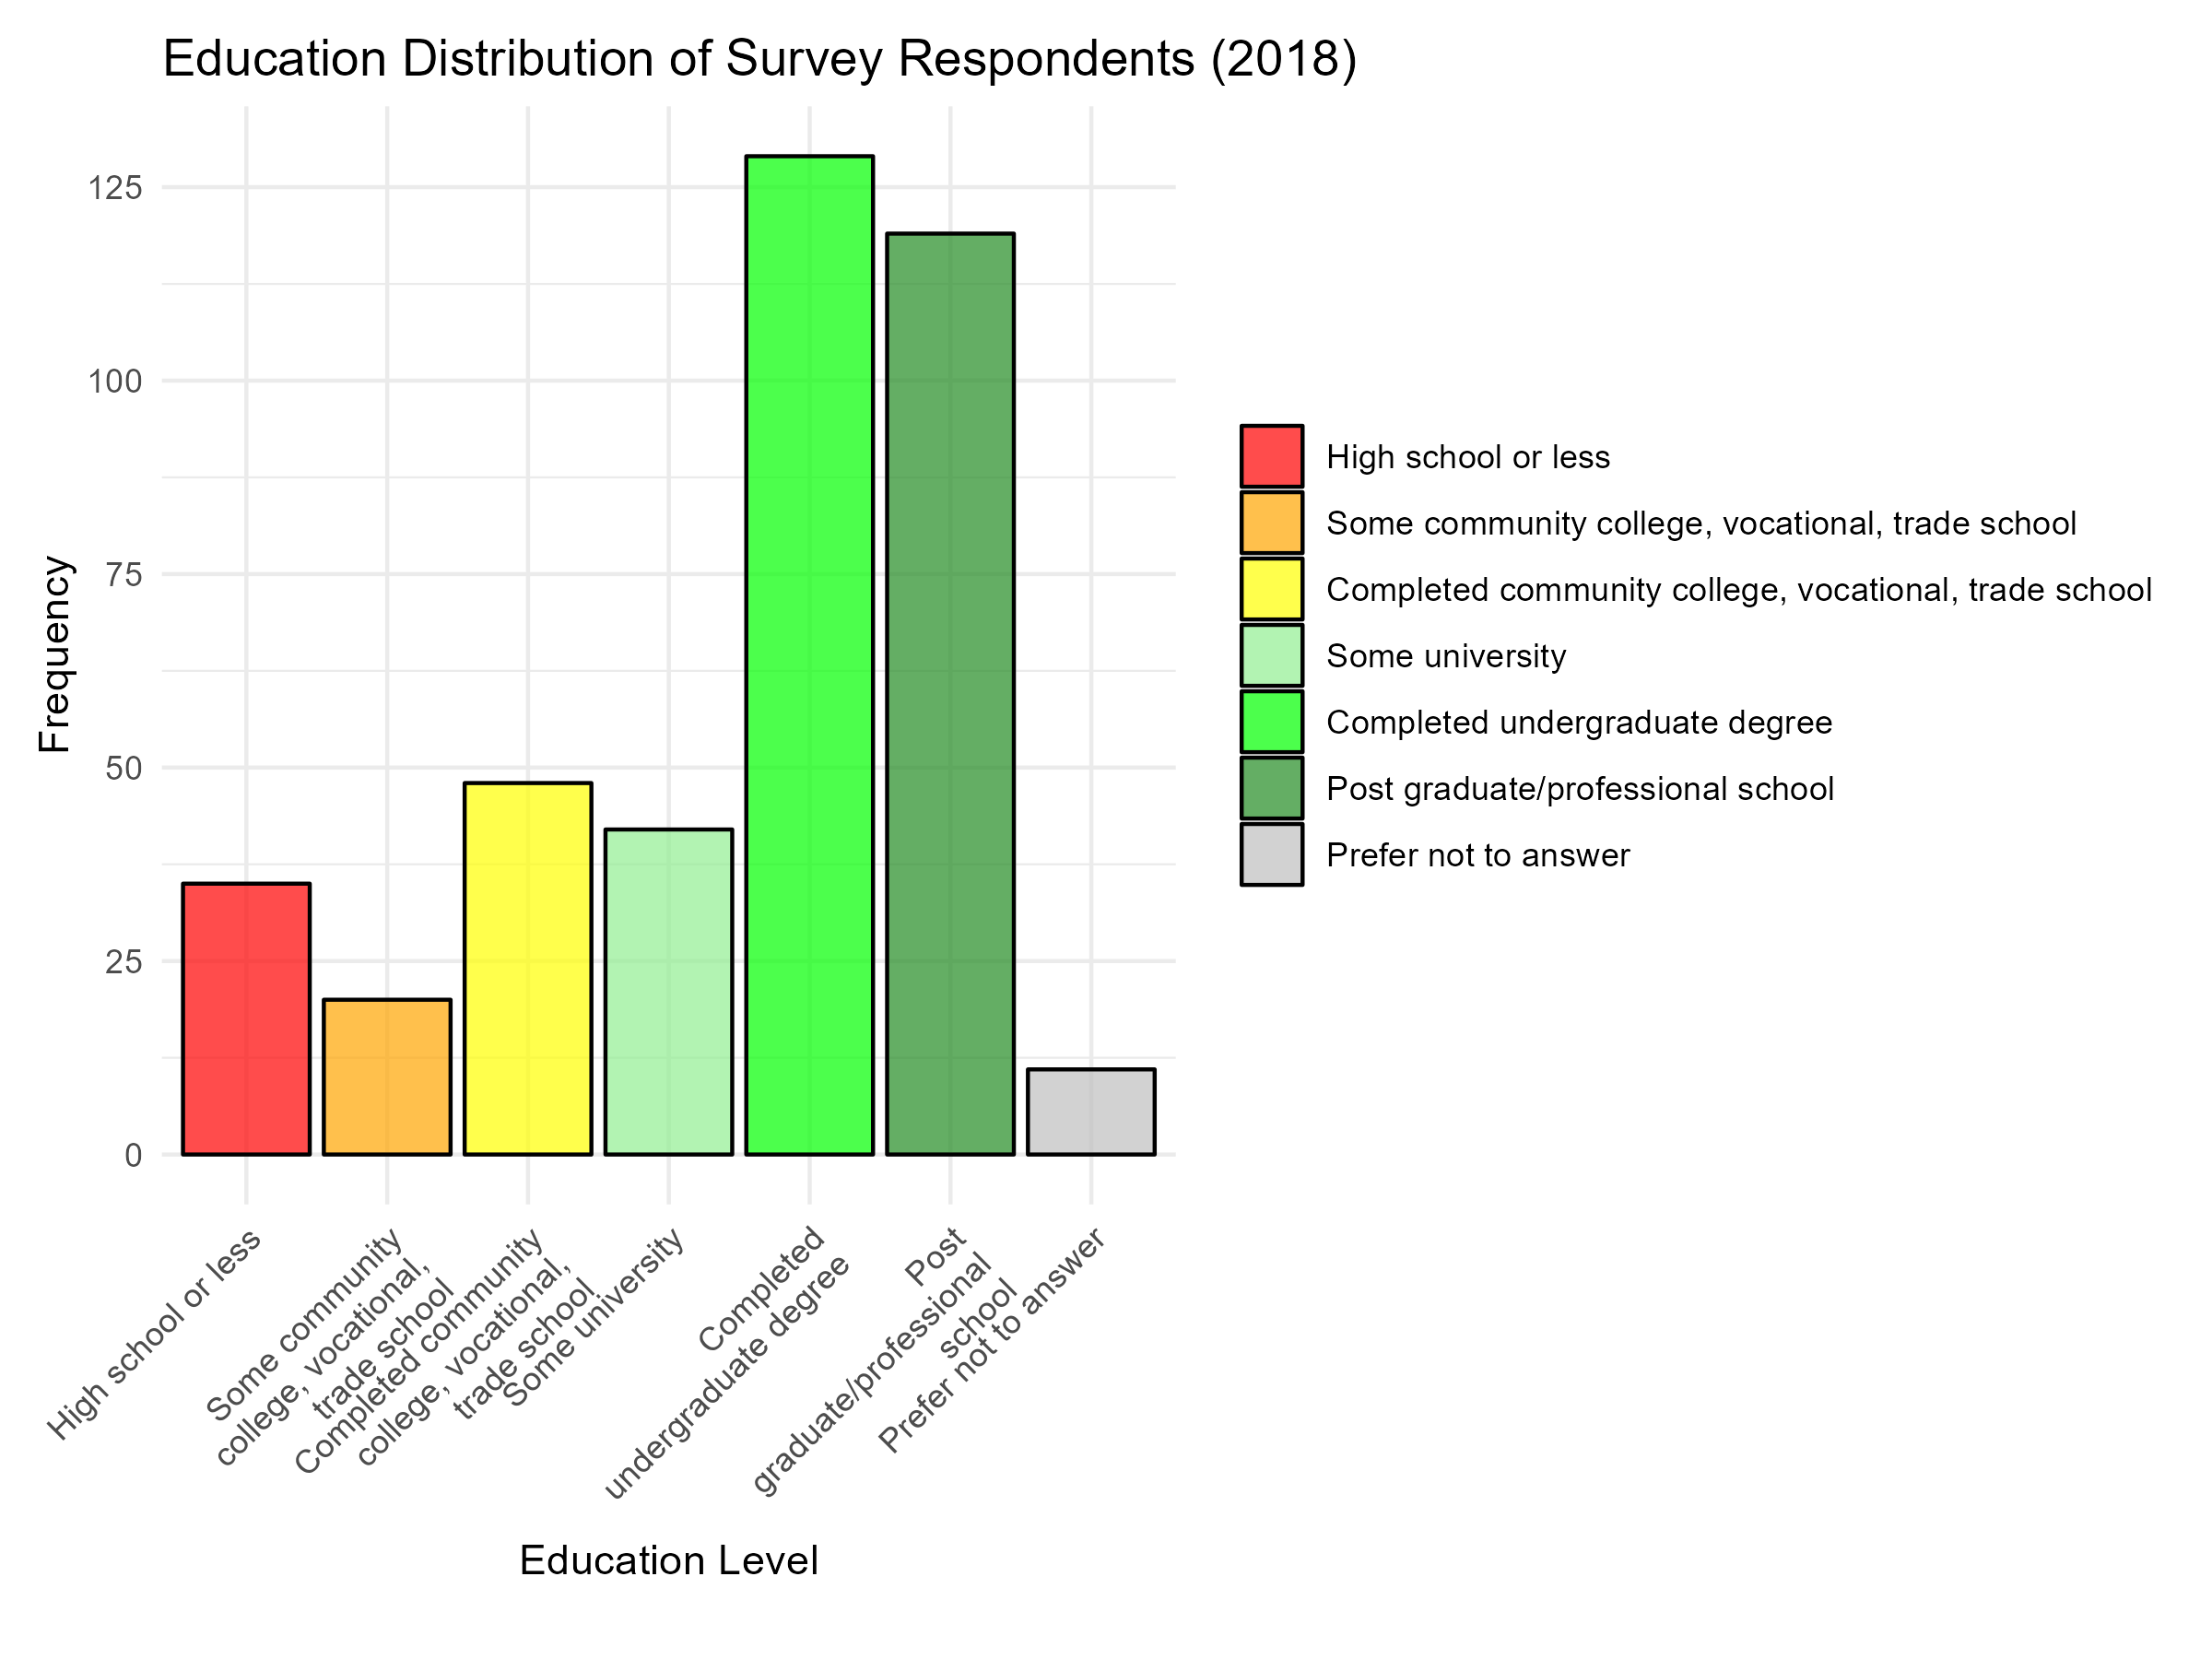
\includegraphics[width=6in,height=\textheight]{../data/03-figures_data/educ_individual_plot.png}

}

\caption{\label{fig-three}The histogram shows the distribution of
education levels of 2018 survey respondents.}

\end{figure}%

\subparagraph{Comparison 2018 to 2021}\label{comparison-2018-to-2021-1}

Figure~\ref{fig-four} compares the education levels of respondents in
2018 and 2021. The two surveys used different education categories,
making direct comparisons challenging. In 2018, 9\% of respondents had a
high school diploma or less, while in 2021, this figure rose to 38\%,
due to the addition of the ``less than high school'' and ``high school
or equivalent'' categories. This shift indicates that the 2021 survey
better represented individuals with lower educational attainment.

The 2018 survey provided more detailed categories, including options for
community college, trade school, and distinctions between ``some''
versus ``completed'' education. In contrast, the 2021 survey used
broader categories, which likely reduced the specificity of educational
data. Notably, the 2021 survey appears to have offered a more balanced
sample, with a wider spread across various education levels, while the
2018 sample was noticeably skewed toward respondents with higher
educational attainment. This suggests that the 2021 survey may have
captured a broader range of educational backgrounds, providing a more
well-rounded representation of Toronto's population.

\begin{figure}

\centering{

\begin{table}
\centering
\begin{tblr}[         %% tabularray outer open
]                     %% tabularray outer close
{                     %% tabularray inner open
colspec={Q[]Q[]Q[]Q[]},
}                     %% tabularray inner close
\toprule
Education Level  & 2018 Percentage & Education Level & 2021 Percentage \\ \midrule %% TinyTableHeader
High school or less                                   &  9 & Less than high school                                                 &  6 \\
Some community college, vocational, trade school      &  5 & High School or equivalent                                             & 32 \\
Completed community college, vocational, trade school & 12 & Degree or diploma from a college or university                        & 26 \\
Some university                                       & 10 & Graduate or professional degree (examples: Master, PhD, MD or LLB/JD) & 35 \\
Completed undergraduate degree                        & 32 & Prefer not to answer                                                  &  1 \\
Post graduate/professional school                     & 29 & DK/NS                                                                 &  0 \\
Prefer not to answer                                  &  3 &                                                                       & NA \\
\bottomrule
\end{tblr}
\end{table}

}

\caption{\label{fig-four}This table highlights the education
distribution of survey respondents in 2018 and 2021.''}

\end{figure}%

\paragraph{Extent Feel Informed}\label{extent-feel-informed}

\subparagraph{Individual 2018}\label{individual-2018-2}

Figure~\ref{fig-five} depicts the distribution of self-reported climate
change knowledge among survey respondents in 2018. The majority of
participants identified as ``Very informed,'' making this the most
prevalent category by a significant margin. A moderate number of
respondents reported being ``Not very informed,'' while a smaller yet
noticeable group described themselves as ``Extremely informed.'' In
contrast, the categories ``Not at all informed'' and ``Not very
informed'' have the lowest frequencies, with ``Not at all informed''
being particularly rare. This distribution suggests that most
respondents possess a relatively high level of awareness about climate
change, with very few indicating a lack of knowledge on the topic.

\begin{figure}

\centering{

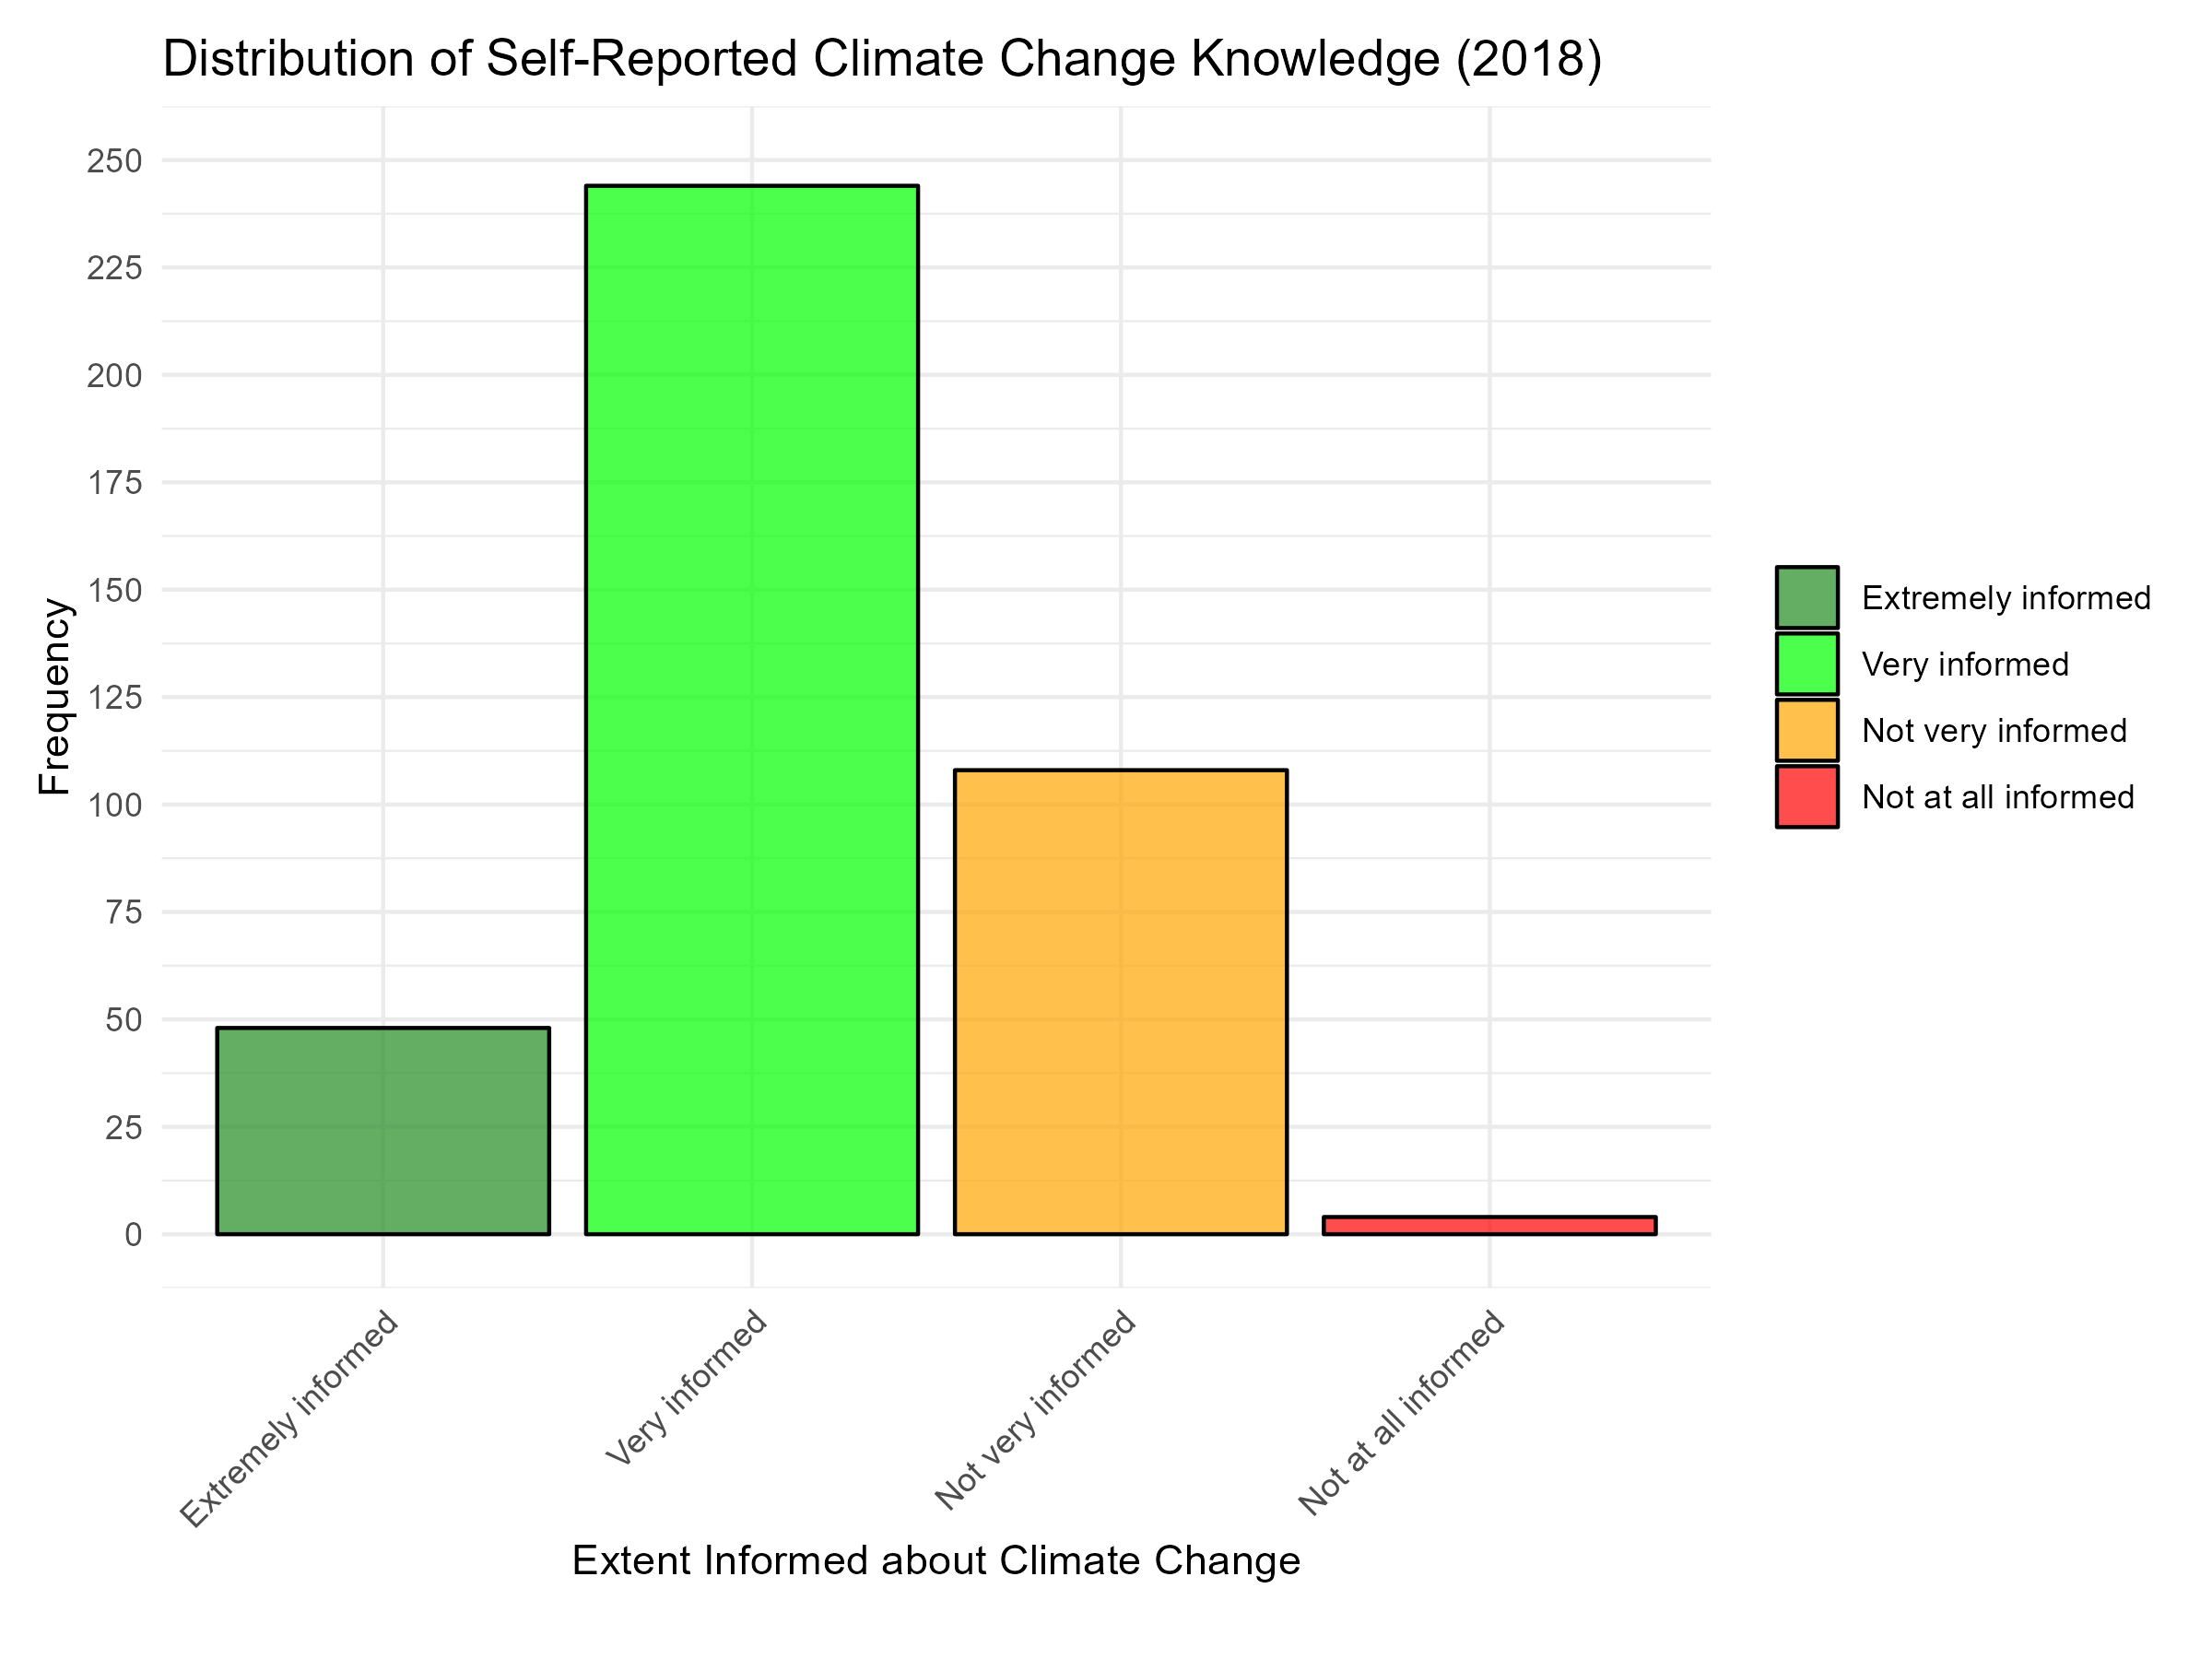
\includegraphics[width=6in,height=\textheight]{../data/03-figures_data/informed_individual_plot.png}

}

\caption{\label{fig-five}The histogram shows the distribution of
self-reported climate change knowledge among 2018 survey respondents.}

\end{figure}%

\subparagraph{Comparison 2018 to 2021}\label{comparison-2018-to-2021-2}

Figure~\ref{fig-six} illustrates the self-reported level of extent
inviduals feel informed about climate change and climate action for 2018
and 2021. In 2018, the large marjority of individuals say they are very
informed with 60 percent and the follwoign category is not very informed
with 27 percent. In 2021, The majority of inividuals also say they are
very informed but to a lesser degree with 48 percent and this is closely
followed by only a little informed with 37 percent. There is a trend
that invidiusls in 2018 reported greater levels of knowldege about
climate change whereas 2021 illstrates a more even split between very
informed and only little informed, portraying that fewer individuals
have adequate knowledge about climate change.

\begin{figure}

\centering{

\begin{table}
\centering
\begin{tabular}[t]{l|l|l|l}
\hline
Extent Informed & 2018 Percentage & Extent Informed & 2021 Percentage\\
\hline
Extremely informed & 12 & Extremely informed & 13\\
\hline
Very informed & 60 & Very informed & 48\\
\hline
Not very informed & 27 & Only a little informed & 37\\
\hline
Not at all informed & 1 & Not at all informed & 2\\
\hline
\end{tabular}
\end{table}

}

\caption{\label{fig-six}This table highlights the extent feel informed
distribution of survey respondents in 2018 and 2021.}

\end{figure}%

\paragraph{Best Method of Delivery}\label{best-method-of-delivery}

\subparagraph{Individual 2018}\label{individual-2018-3}

Figure~\ref{fig-seven}, shows 2018 survey results for the preferred
method for receiving climate change information. Advertising campaigns
emerged as the most popular choice, selected by approximately 55 percent
of respondents, followed closely by newsletters with 52 percent and the
Toronto.ca website with 46 percent. On the other hand, social media
platforms such as Facebook, Instagram, and Twitter were less popular
overall, with Twitter 12 percent and Instagram 17 percent garnering the
fewer votes. Notably, only 5 percent of respondents reported being
uninterested in receiving information about climate action. These
findings suggest that more traditional communication methods, such as
advertising and newsletters, resonated better with respondents compared
to social media.

\begin{figure}

\centering{

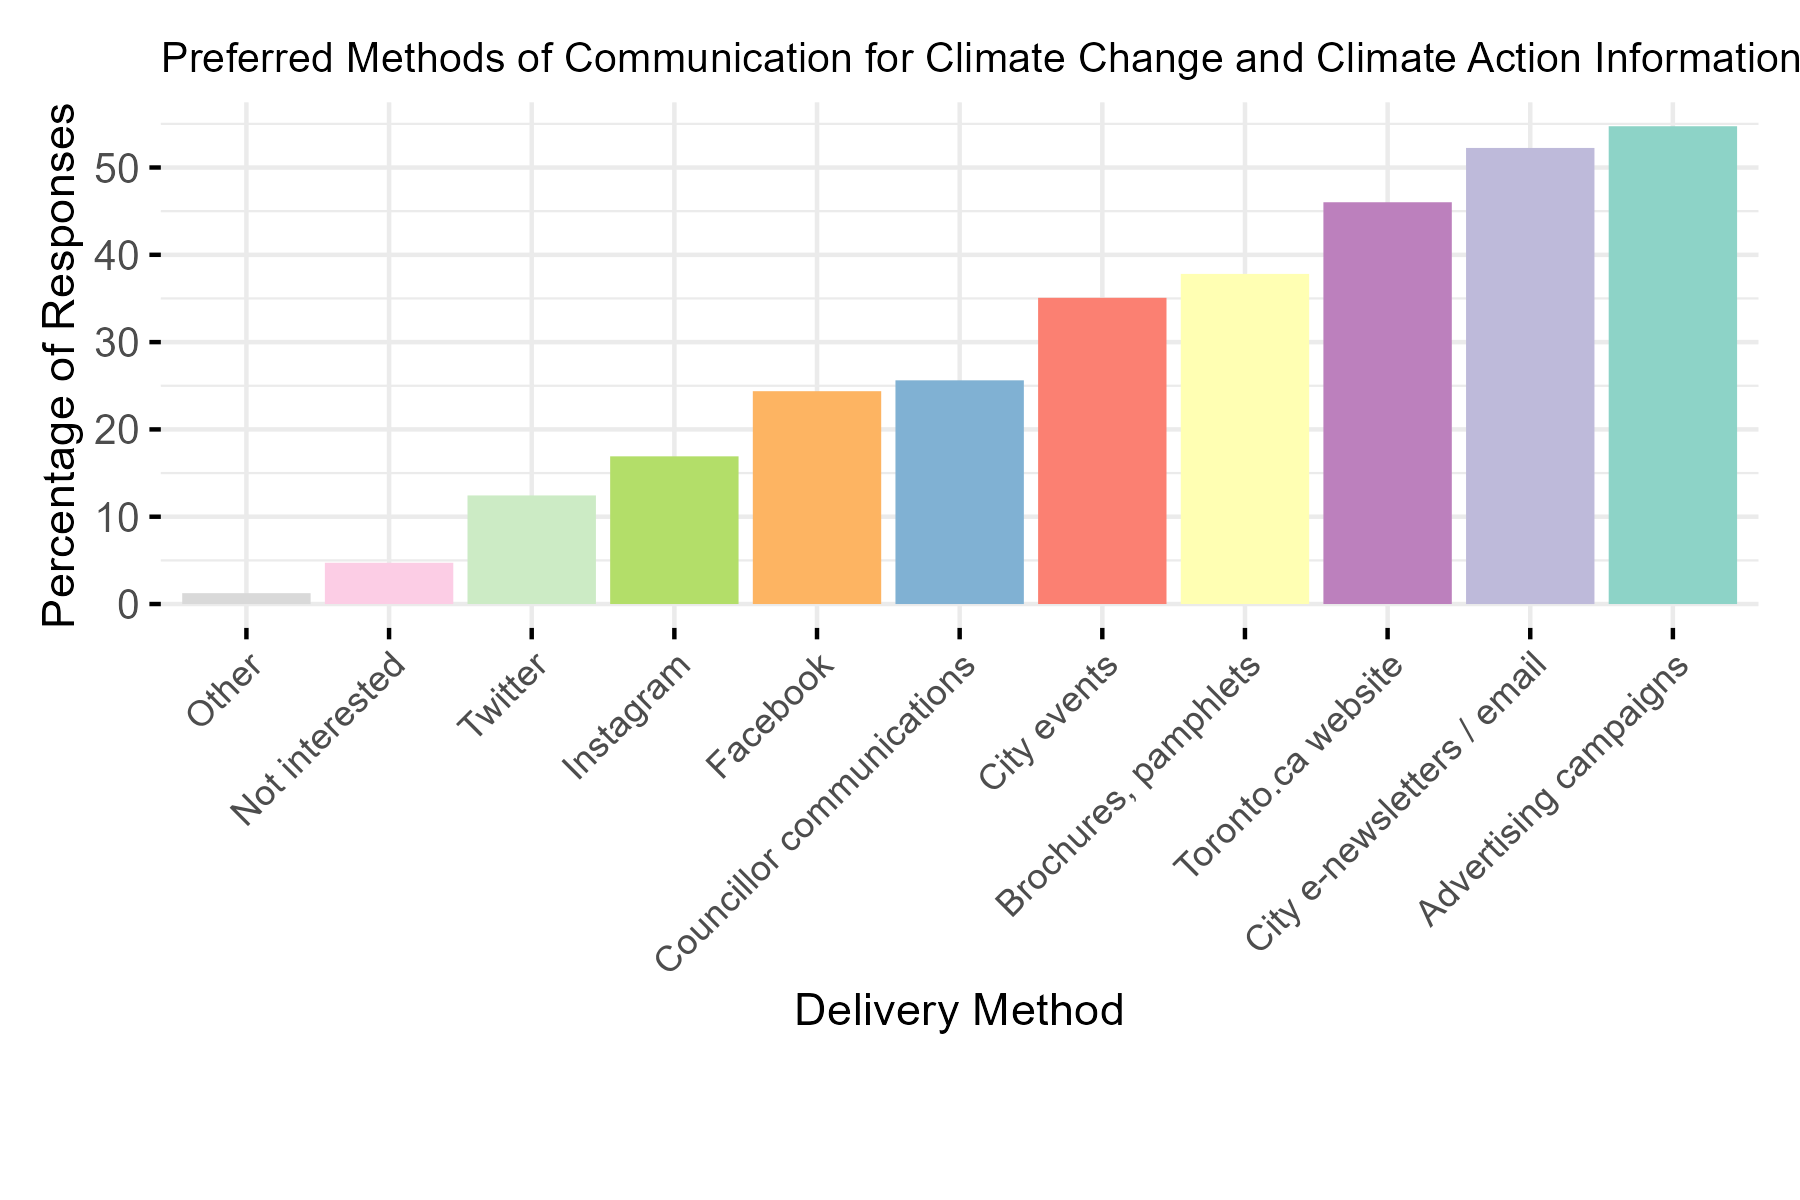
\includegraphics[width=6in,height=\textheight]{../data/03-figures_data/communication_18_plot.png}

}

\caption{\label{fig-seven}The stacked bar plot illustrates the preferred
methods of communication for receiving information about climate change
and climate action.}

\end{figure}%

\subparagraph{Comparison 2018 to 2021}\label{comparison-2018-to-2021-3}

Figure~\ref{fig-eight} compares the preferred methods of delivering
climate change information between the 2018 and 2021 surveys. While the
top three methods namely advertising campaigns, newsletters, and the
Toronto.ca website remained consistent across both years, there were
notable shifts in preferences. Traditional methods such as newsletters,
advertising campaigns, brochures, and pamphlets saw a decline in 2021.
In contrast, social media platforms including Twitter, Facebook, and
Instagram gained traction, reflecting a growing reliance on digital
communication channels.

Additionally, the 2021 survey introduced new categories, including the
BetterHomesTO.ca website, which accounted for 15 percent of responses.
This addition underscores the increasing importance of specialized
online platforms in engaging the public on climate action. These changes
highlight a shift toward more diverse and digitally focused
communication strategies over time.

\begin{figure}

\centering{

\begin{table}
\centering
\begin{tabular}[t]{l|l|l|l}
\hline
Communication Method & 2018 Percentage & Communication Method & 2021 Percentage\\
\hline
Toronto.ca website & 46 & Toronto.ca website & 44\\
\hline
Events & 35 & City of Toronto events & 31\\
\hline
Twitter & 13 & Twitter & 17\\
\hline
Facebook & 25 & Facebook & 26\\
\hline
Instagram & 17 & Instagram & 25\\
\hline
Enewsletter / email & 52 & City of Toronto e-newsletters / email & 43\\
\hline
Councillor communication & 25 & Councillor e-newsletters & 24\\
\hline
Advertising campaigns & 55 & Advertising campaigns & 42\\
\hline
Brochures / Pamphlets & 38 & Printed or online brochures, pamphlets & 31\\
\hline
Other & 1 & BetterHomesTO.ca website & 15\\
\hline
Not interested & 5 & Not interested in receiving information & 8\\
\hline
 &  & Mail/ letter & 1\\
\hline
 &  & Nothing & 1\\
\hline
 &  & Other & 0\\
\hline
 &  & Don't know & 0\\
\hline
\end{tabular}
\end{table}

}

\caption{\label{fig-eight}This table highlights the prefered method of
communication of survey respondents in 2018 and 2021.}

\end{figure}%

\paragraph{Likelihood Taking Action}\label{likelihood-taking-action}

Figure~\ref{fig-nine} illustrates the self-reported likelihood of
individuals taking various actions to minimize environmental impacts.
The x-axis displays nine different climate actions, while the y-axis
represents the percentage of individuals corresponding to each
likelihood level. A stacked bar chart is used to visualize the
distribution of responses, with a color-coded legend ranging from green
(high likelihood of action) to red (low likelihood of action).

Sorting waste into the correct bins is the most frequently reported
action that individuals are currently undertaking, accounting for 60
percent of responses. Other common actions individuals are already
participating in include walking or cycling short distances with 40
percent, reducing waste by contributing to the repurposing of used
products with 37 percent and reducing hydro usage with 36 percent

In contrast, the least popular actions include switching to electric or
hybrid vehicles, with 14 percent of respondents reporting they are very
unlikely to take this action and 27 percent stating they are somewhat
unlikely. Similarly, consuming less meat by incorporating more
plant-based foods is unpopular, with 12 percent reporting they are very
unlikely and 23 percent somewhat unlikely to adopt this change.
Minimizing car use is another action with low reported likelihood, with
10 percent of respondents very unlikely and 16 percent somewhat unlikely
to reduce their car usage.

\begin{figure}

\centering{

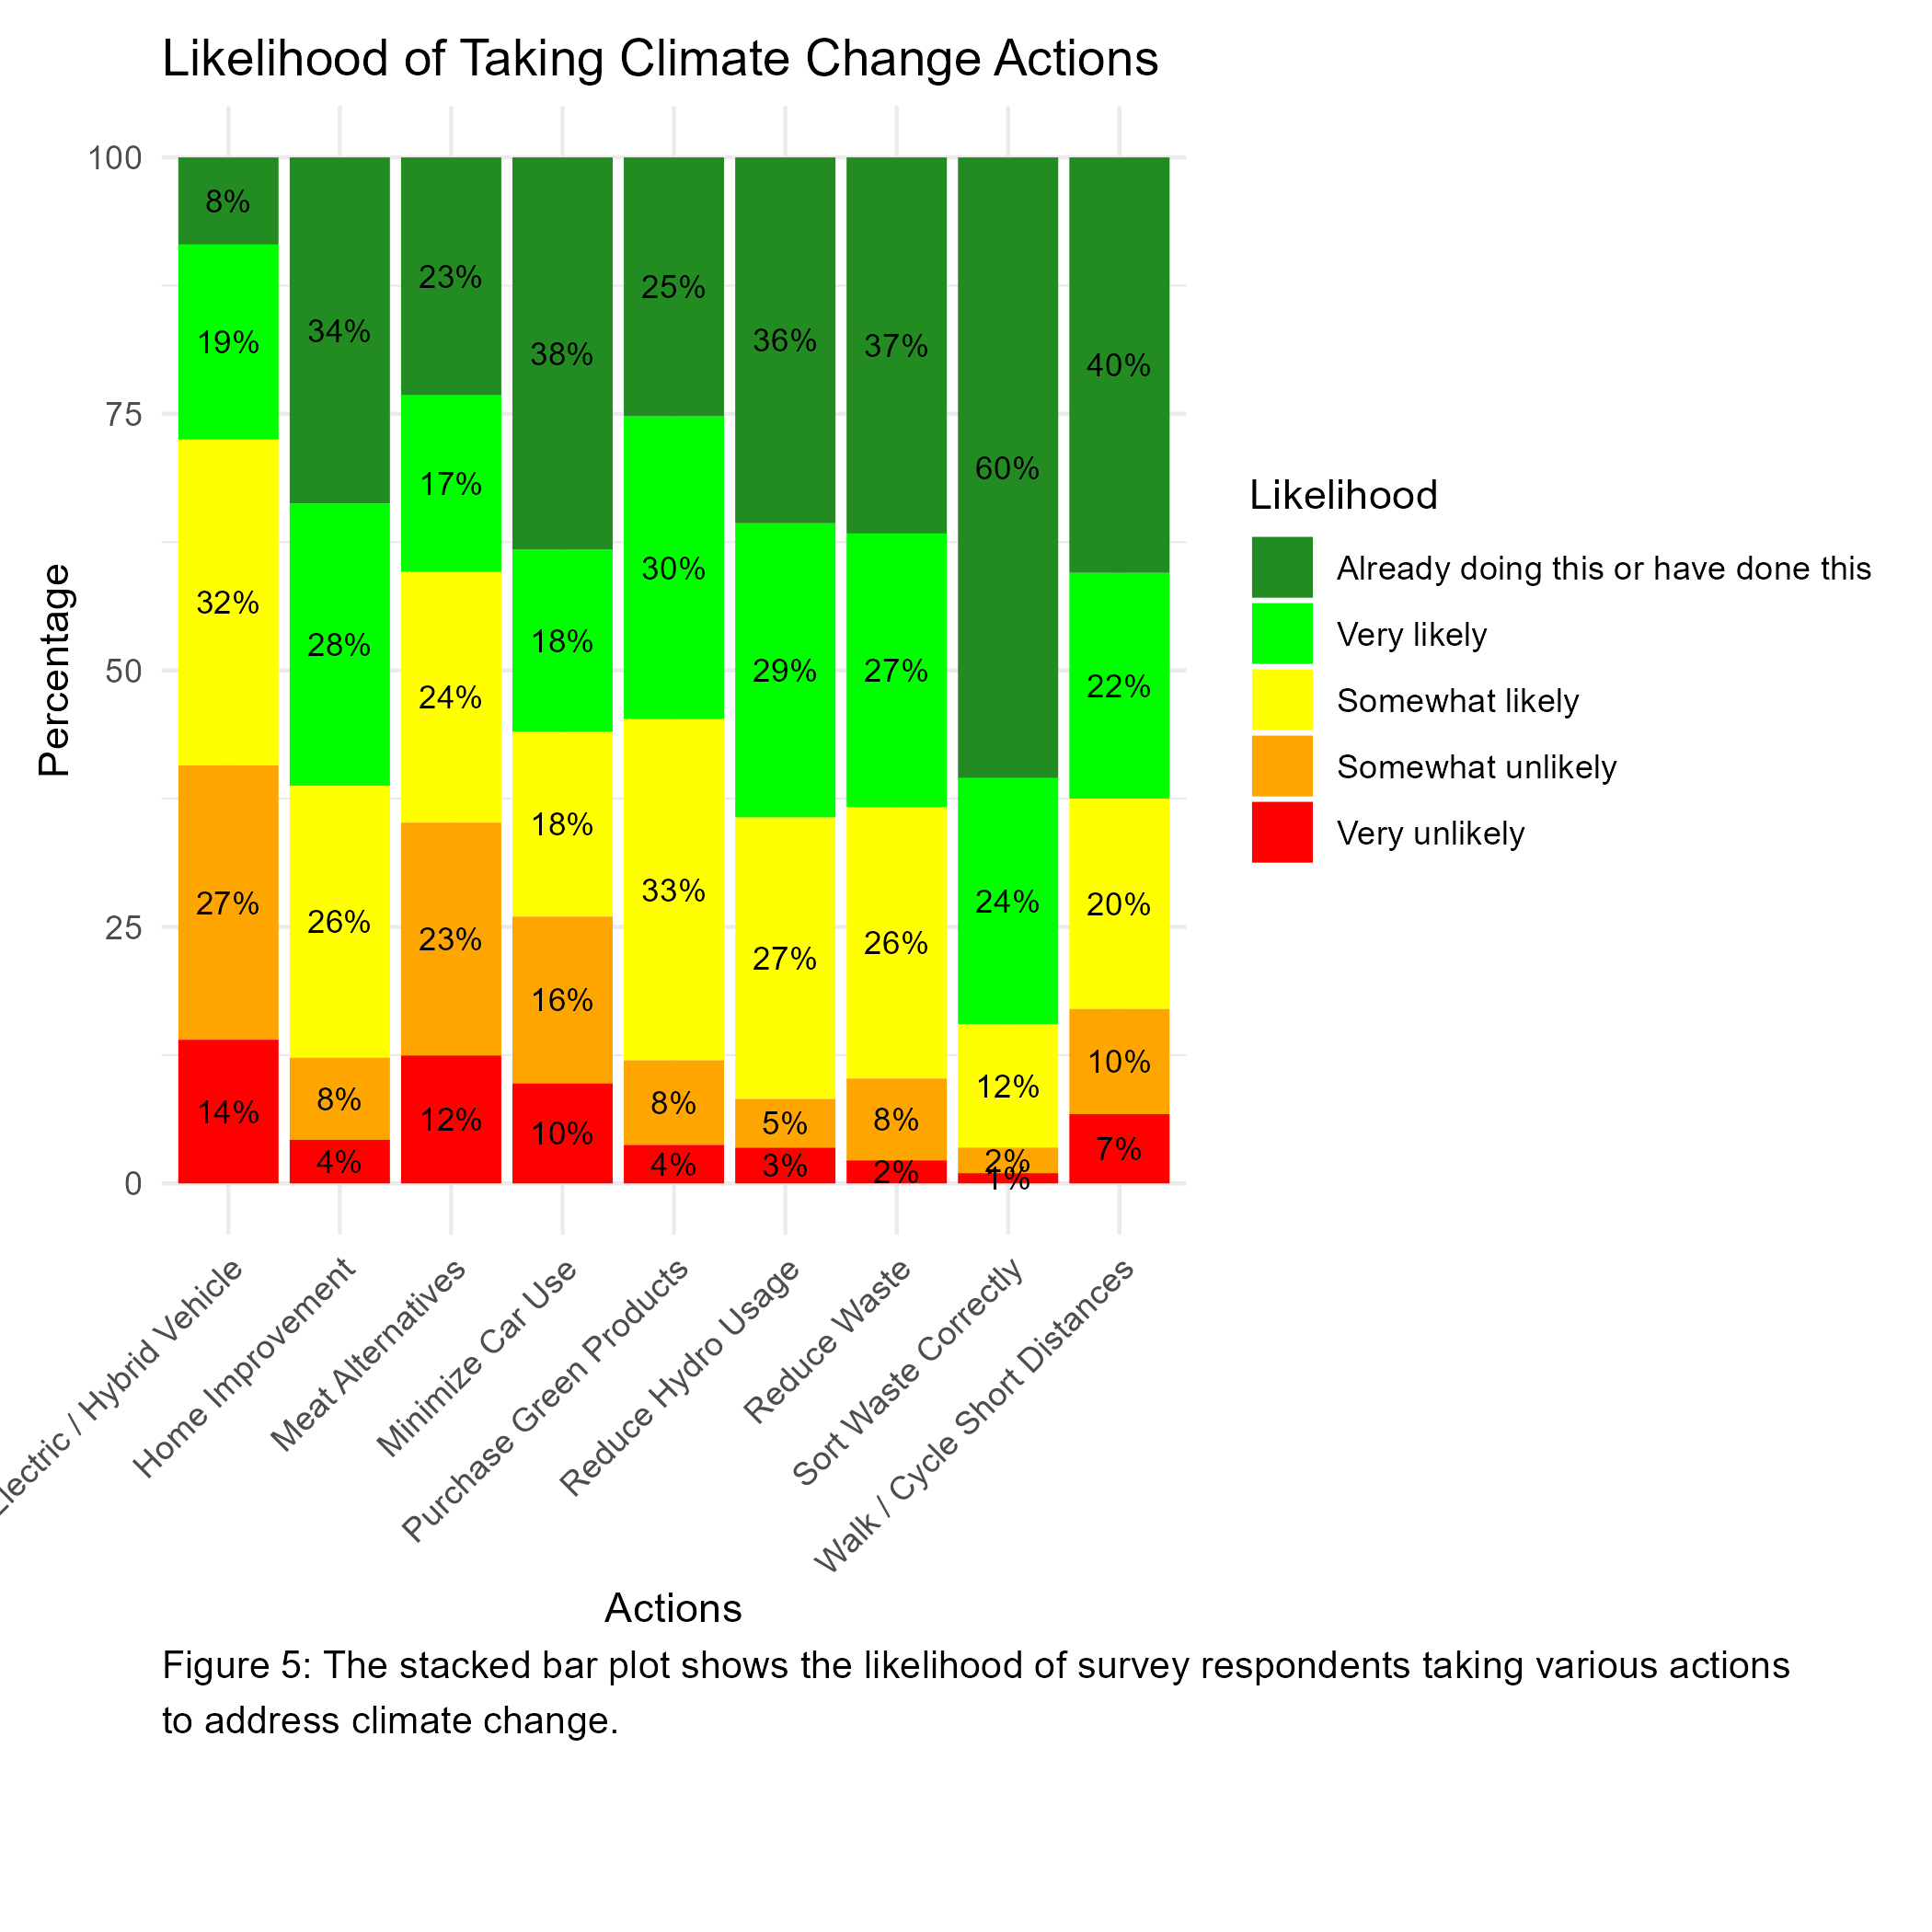
\includegraphics[width=6in,height=\textheight]{../data/03-figures_data/likelihood_individual_plot.png}

}

\caption{\label{fig-nine}The stacked bar plot shows the likelihood of
survey respondents taking various actions to address climate change.}

\end{figure}%

\subsection{Model}\label{sec-model}

The goal of our modeling strategy is twofold: first, to predict how
demographic factors influence individuals' likelihood of engaging in
climate-friendly behaviors, and second, to uncover the role of age and
education in shaping these actions. The actions considered include
investing in electric vehicles, reducing hydro usage, adopting meat
alternatives, and walking or cycling shorter distances. We use a
decision tree model to provide a clear, interpretable framework for
analyzing these relationships.

\subsection{Model set-up}\label{model-set-up}

Our model predicts the likelihood of engaging in specific
climate-positive actions, with age and education level serving as
predictors. Likelihood is measured on a five-point scale, ranging from
``Already doing this or have done this'' to ``Very unlikely.''

\subsubsection{Model Specifications}\label{model-specifications}

We employ separate decision tree models for each action. Age
(continuous) and education (categorical) are the key predictors driving
predictions. Each tree splits the data at nodes based on these
variables, revealing demographic conditions associated with greater or
lesser likelihoods of climate-positive behaviors.

\subsubsection{Model Justification}\label{model-justification}

This approach provides insights into how demographic factors influence
climate-friendly actions, including energy reduction, sustainable
practices, and green technology adoption. By identifying demographic
groups more likely to take these actions, the model can inform targeted
interventions.

\paragraph{Response Variable}\label{response-variable}

The response variable measures the likelihood of engaging in specific
climate-friendly behaviors, represented on a five-point scale: ``Already
doing this or have done this,'' ``Very likely,'' ``Somewhat likely,''
``Somewhat unlikely,'' and ``Very unlikely.'' This scale reflects an
individual's readiness to adopt sustainable practices.

\paragraph{Input Variables}\label{input-variables}

Our predictors are:

\begin{itemize}
\item
  \textbf{Age}: Research shows that younger individuals often
  demonstrate greater environmental awareness and a stronger inclination
  toward sustainable actions (Leiserowitz et al., 2010; Gifford, 2013).
\item
  \textbf{Education}: Previous studies illustrate that higher education
  correlates with increased environmental awareness and sustainable
  behavior adoption (Kollmuss \& Agyeman, 2002).
\end{itemize}

\paragraph{Model Structure}\label{model-structure}

The decision tree splits data based on age and education, uncovering
demographic patterns in climate-positive behaviors. Unlike linear
models, decision trees do not assume direct relationships but instead
identify conditions under which certain behaviors are more likely to
occur. This assumption of independence allows clear interpretation of
each factor's influence.

\subsection{Understanding Decision
Trees}\label{understanding-decision-trees}

Decision trees predict outcomes by recursively splitting data based on
predictor variables. Starting at the root node (entire dataset), the
tree branches into nodes based on decision rules, ultimately reaching
terminal nodes that represent specific predictions, such as the
likelihood of adopting sustainable behaviors. Each split aims to
maximize prediction accuracy, and error rates indicate the reliability
of classifications.

\subsubsection{Decision Trees for Climate-Friendly
Actions}\label{decision-trees-for-climate-friendly-actions}

We fit nine decision tree models to predict the likelihood of the
following climate-friendly actions, using age and education as
predictors:

\begin{enumerate}
\def\labelenumi{\arabic{enumi}.}
\tightlist
\item
  Likelihood of switching in an electric or hybrid vehicle
\item
  Likelihood of minimizing car use
\item
  Likelihood of walking or cycling shorter distances
\item
  Likelihood of purchasing green products
\item
  Likelihood of reducing waste by repurposing used product
\item
  Likelihood of sorting waste correctly
\item
  Likelihood of making home improvements
\item
  Likelihood of adopting meat alternatives
\item
  Likelihood of reducing hydro usage
\end{enumerate}

Each model follows a consistent structure, highlighting how age and
education influence these behaviors.

\subsection{Model Estimation and
Interpretation}\label{model-estimation-and-interpretation}

The model predicts that younger individuals with higher education levels
are more likely to adopt climate-friendly behaviors. The decision tree
identifies key splits in the data and evaluates prediction reliability
using error rates, providing insight into the impact of age and
education on sustainable actions.

\subsubsection{Transportation Actions}\label{transportation-actions}

\paragraph{Likelihood of switching to an electric or hybrid
vehicle}\label{likelihood-of-switching-to-an-electric-or-hybrid-vehicle}

Figure~\ref{fig-ten} reveals that education is the primary predictor for
the likelihood of switching to an electric or hybrid vehicle.
Individuals with ``Some Community/Trade School'' or ``Some University''
education are ``Very likely'' to invest, though with moderate
variability (error rate 63.8\%). Those with higher education show more
age-based segmentation. Younger individuals under 35 years are more
likely to invest, with a lower error rate (30\%). Older individuals,
particularly those over 69 years, are ``Very unlikely'' to invest. This
model demonstrates how age and education interact to influence vehicle
choice.

\begin{figure}

\centering{

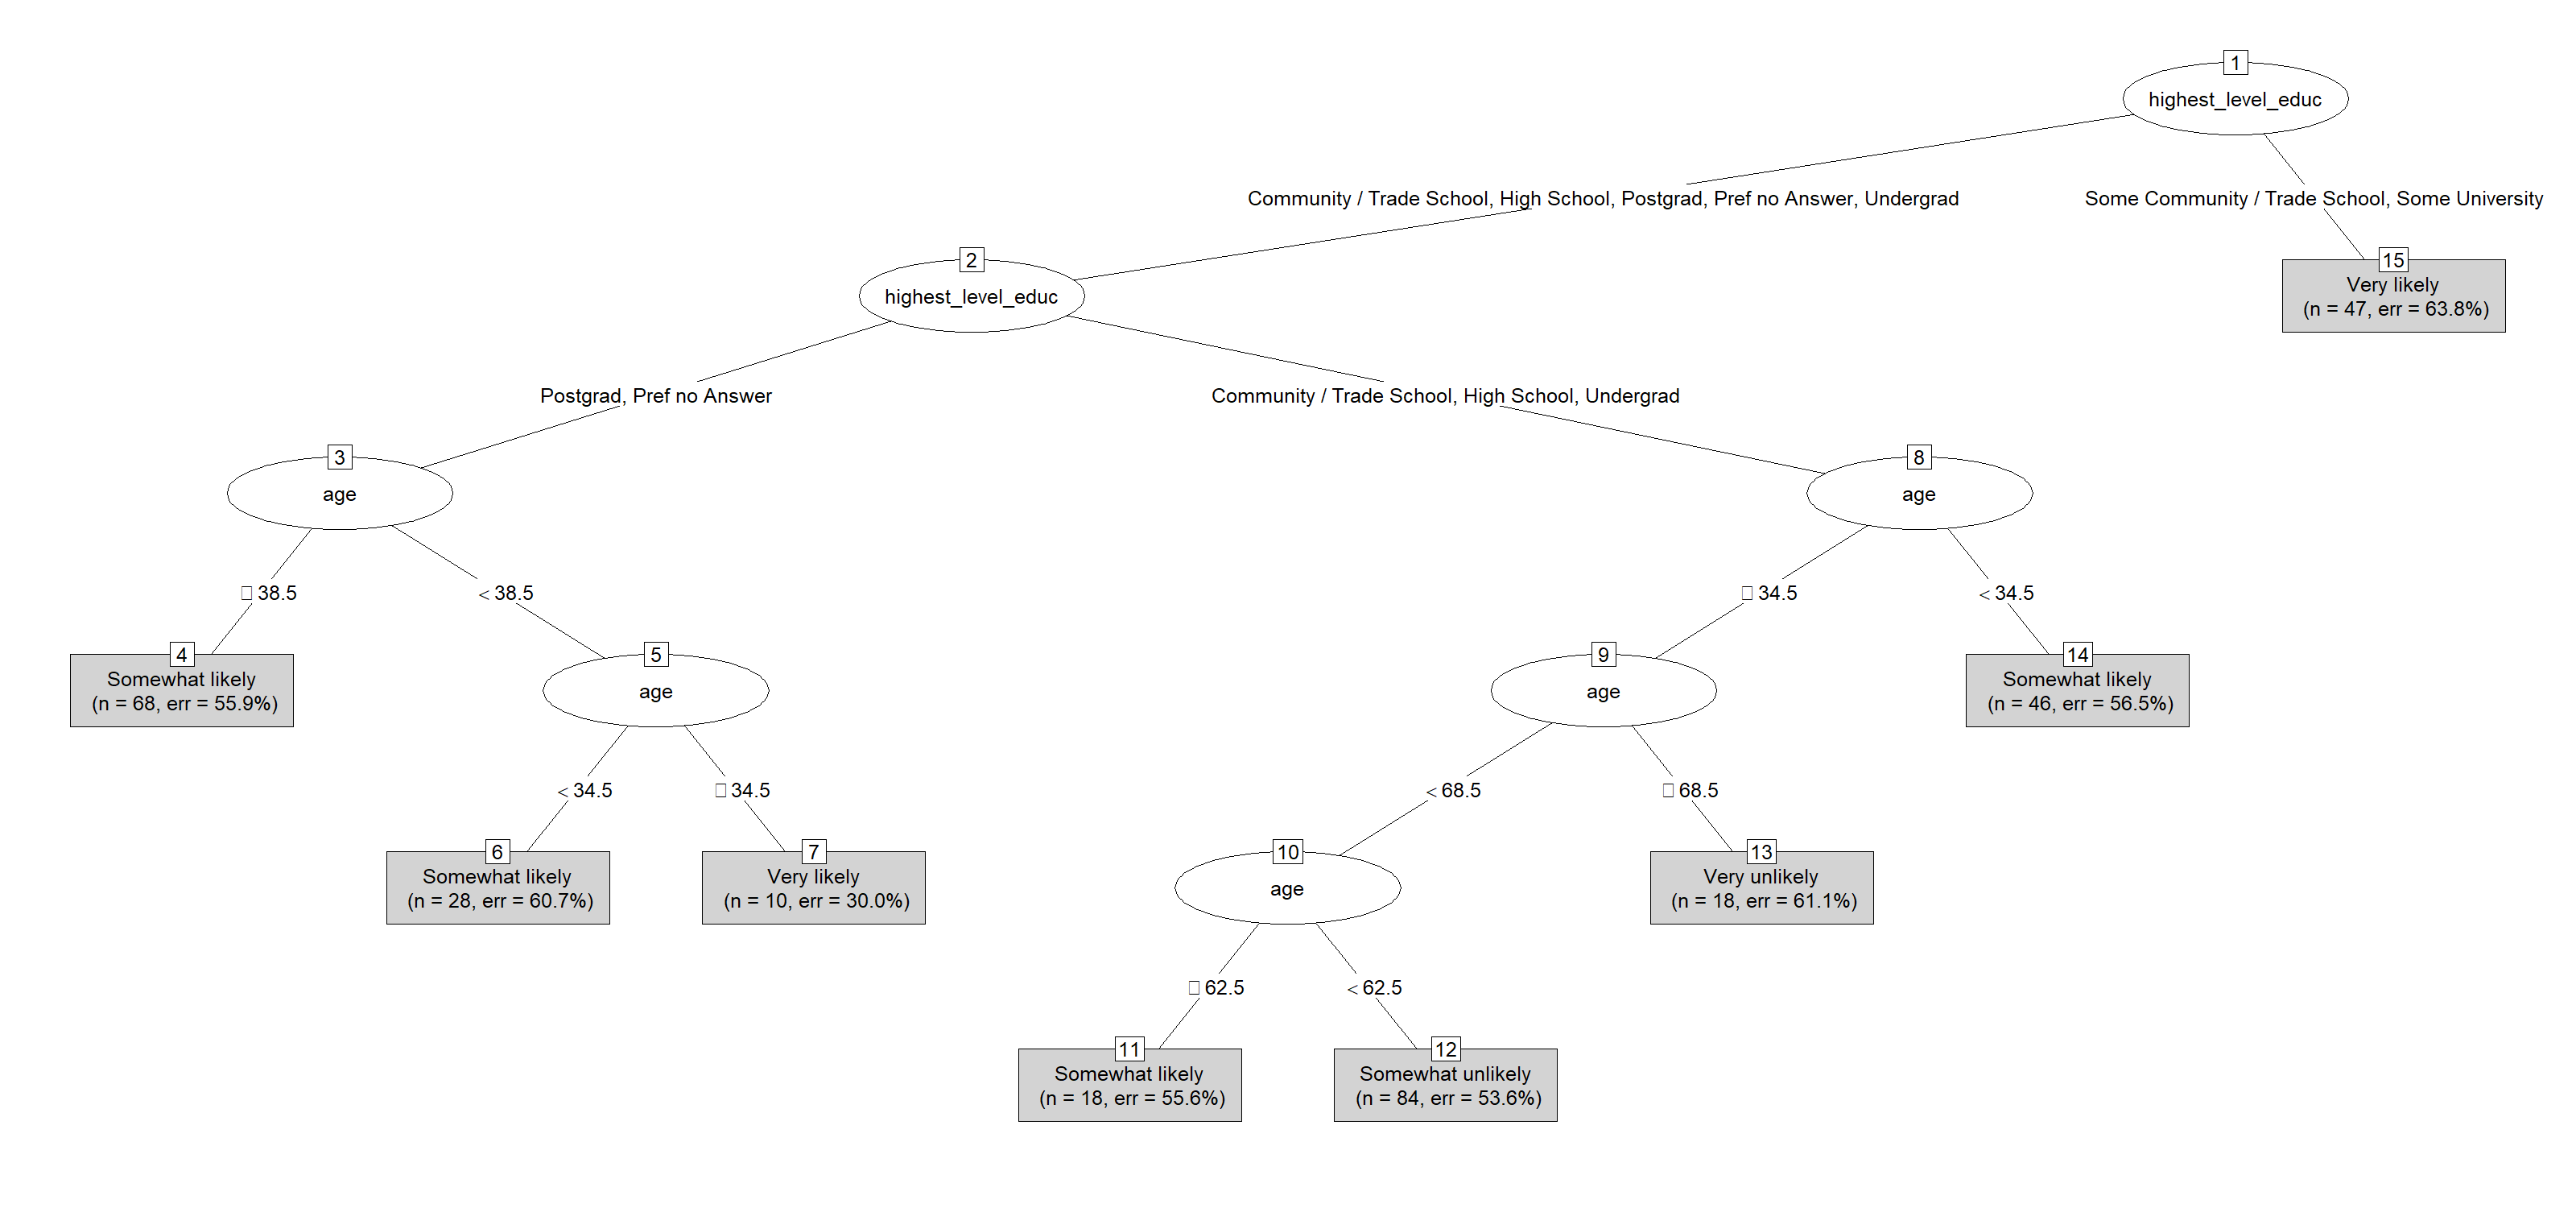
\includegraphics[width=10.67in,height=\textheight]{../models/vehicle_electric_tree.png}

}

\caption{\label{fig-ten}Probability tree for likelihood of investing in
an electric or hybrid vehicle, predicted by age and education.}

\end{figure}%

\paragraph{Likelihood of minimizing car
use}\label{likelihood-of-minimizing-car-use}

Figure~\ref{fig-eleven} shows that the likelihood of minimizing car use
is consistent across the sample, with a high error rate (61.9\%). The
model classifies all individuals into the ``Already doing this or have
done this'' category, indicating widespread adoption of this behavior,
regardless of age or education

\begin{figure}

\centering{

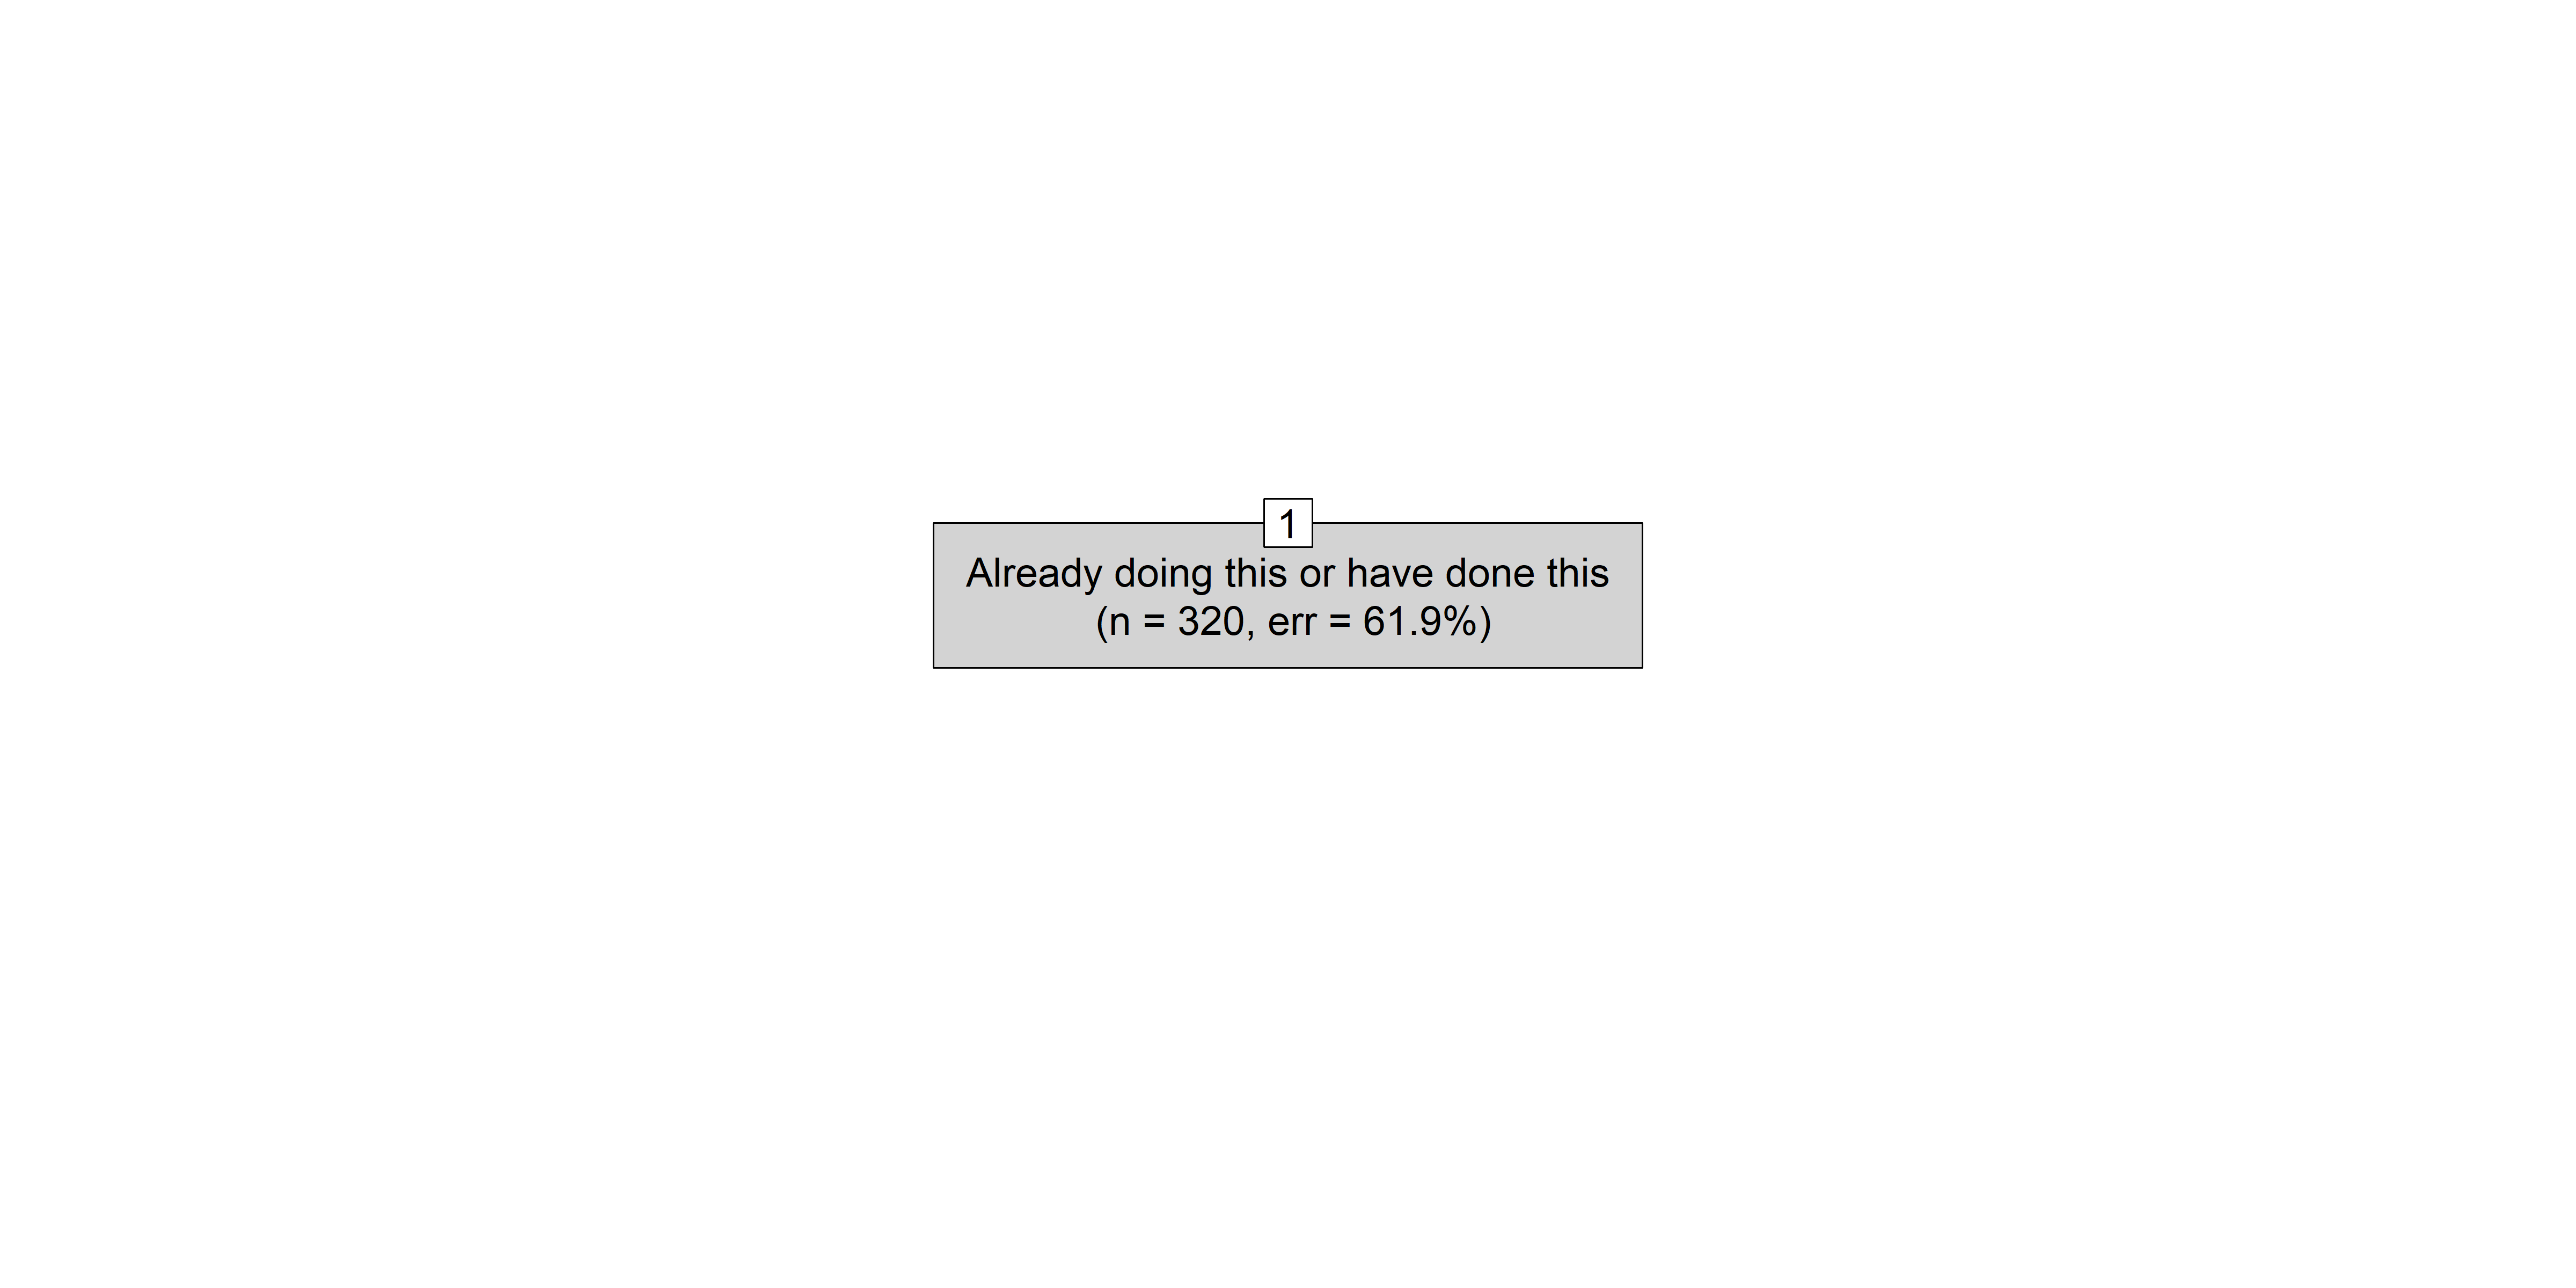
\includegraphics[width=10.67in,height=\textheight]{../models/minimize_car_tree.png}

}

\caption{\label{fig-eleven}Probability tree for likelihood of minimizing
car use, predicted by age and education.}

\end{figure}%

\paragraph{Likelihood of walking or cycling shorter
distances}\label{likelihood-of-walking-or-cycling-shorter-distances}

Figure~\ref{fig-twelve} indicates that education is the primary factor
influencing short-distance walking or cycling. Those with higher
education (postgraduate, undergraduate, or some university) are more
likely to engage in this behavior, with an error rate of 51.9\%. For
those with lower education, age plays a significant role, with younger
individuals (under 66 years) more likely to walk or cycle, with an error
rate of 60\%. This model highlights how education and age together shape
short-distance mobility, with error rates reflecting the model's
predictive variability.

\begin{figure}

\centering{

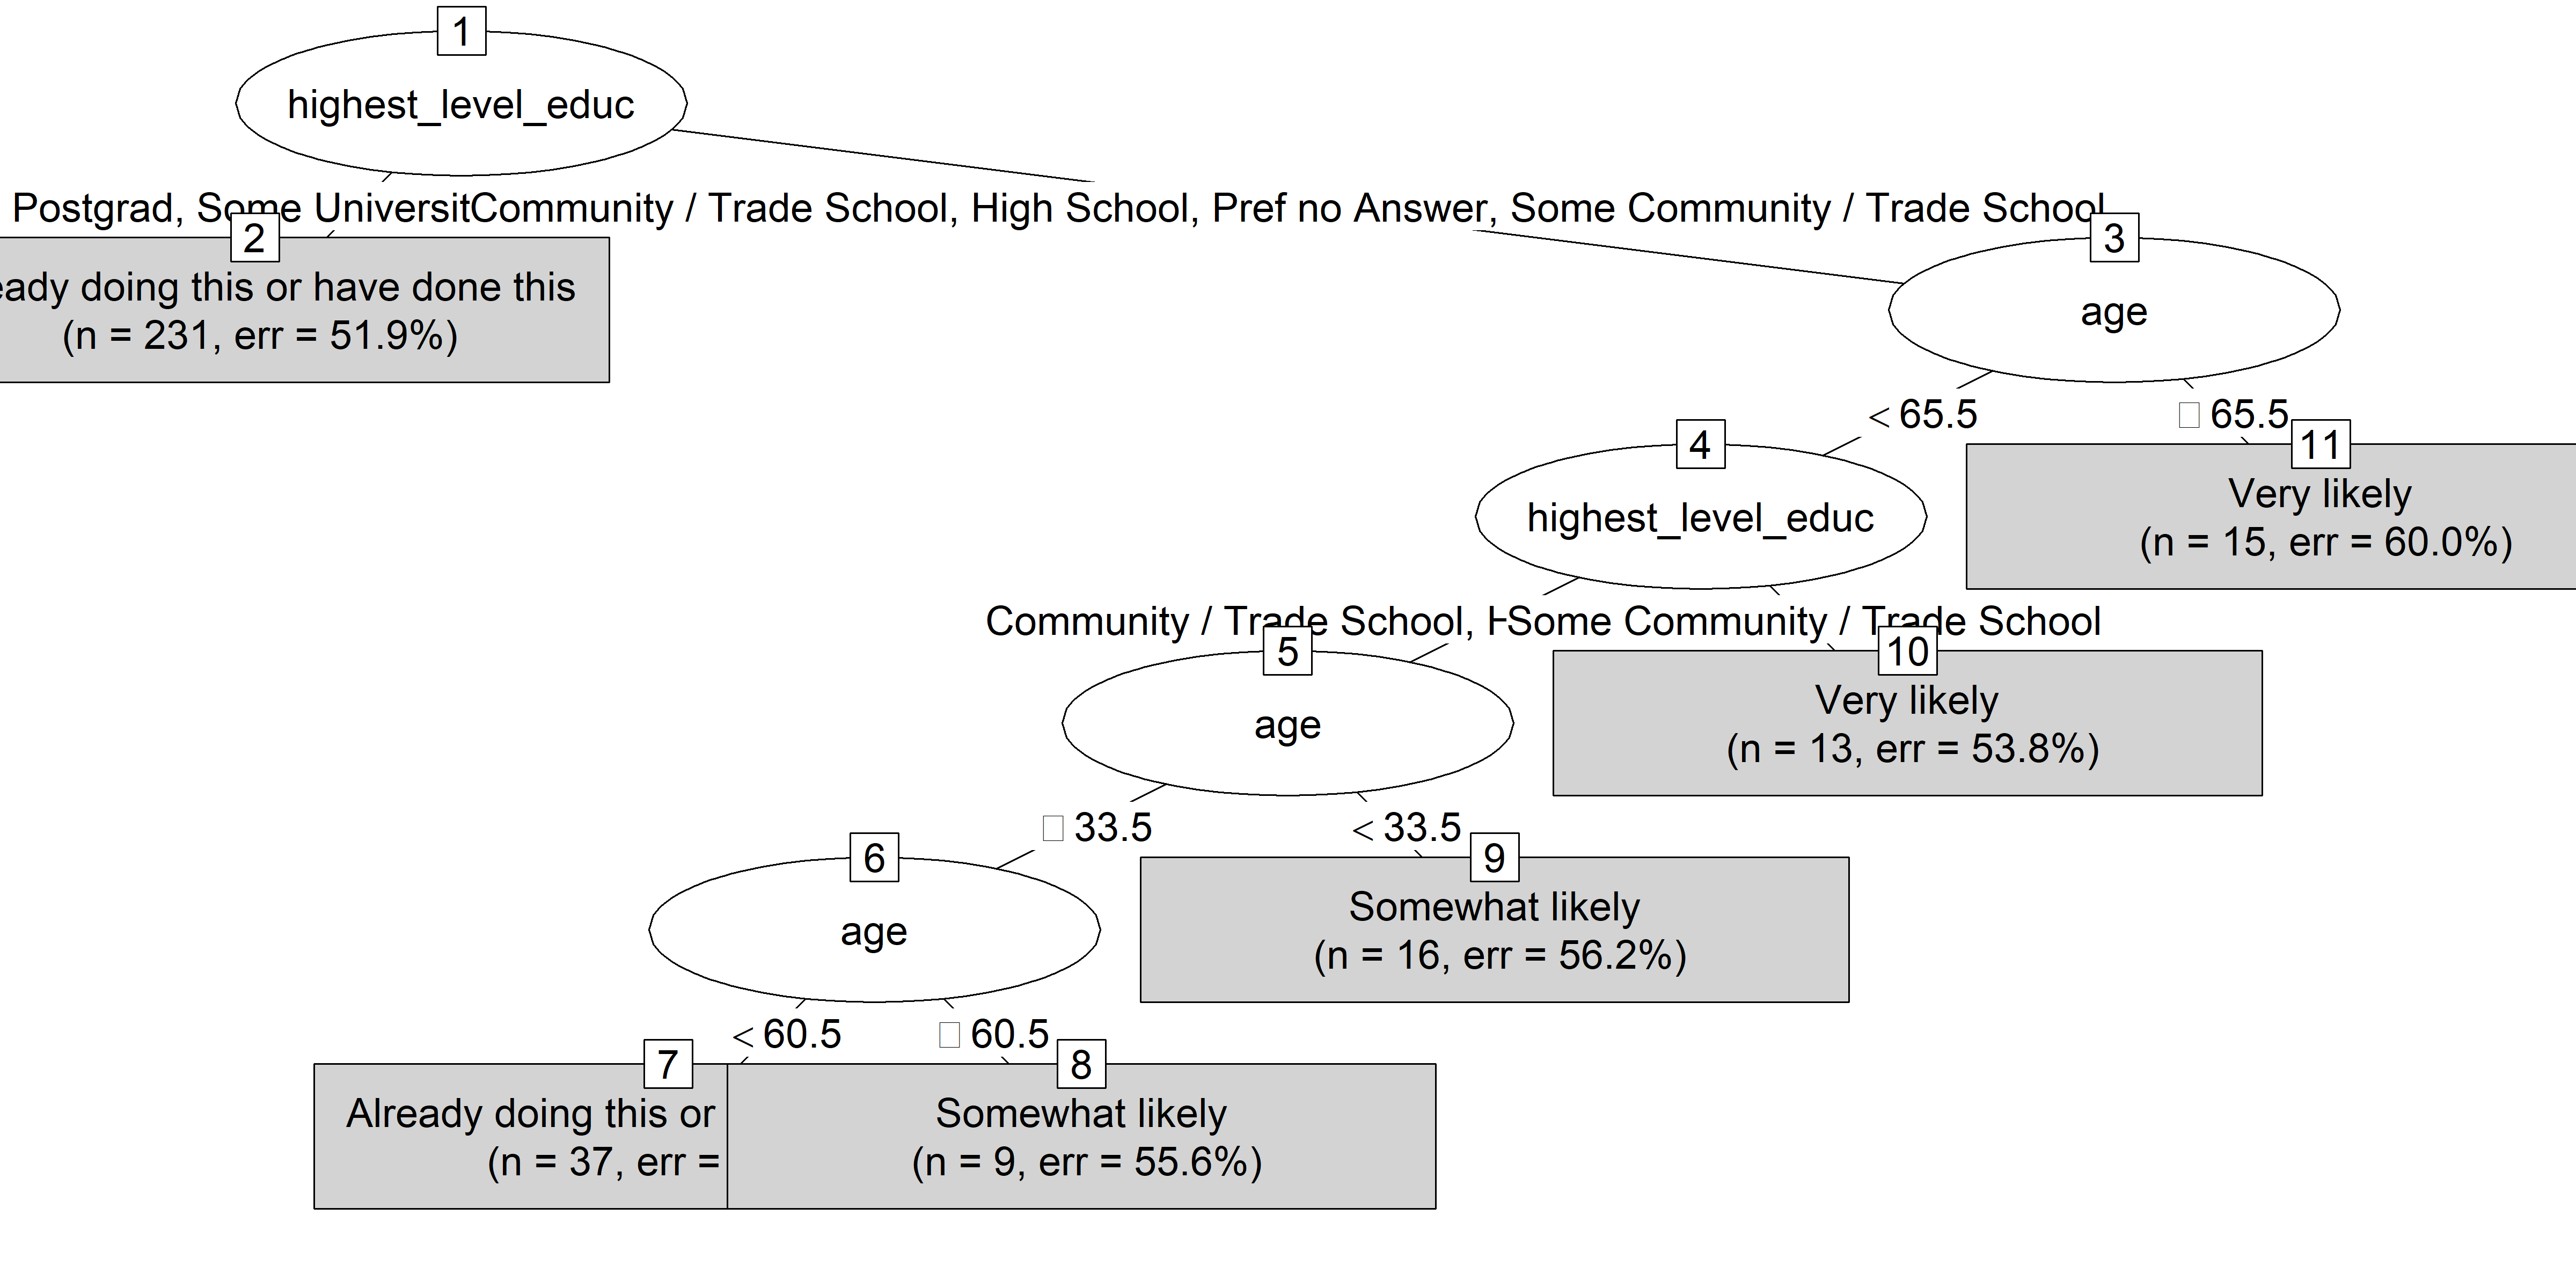
\includegraphics[width=10.67in,height=\textheight]{../models/short_distance_tree.png}

}

\caption{\label{fig-twelve}Probability tree for likelihood of walking or
cycling shorter distances, predicted by age and education.}

\end{figure}%

\subsubsection{Waste and Product
Actions}\label{waste-and-product-actions}

\paragraph{Likelihood of purchasing green
products}\label{likelihood-of-purchasing-green-products}

Figure~\ref{fig-thirteen} reveals that age is the initial split for
green product purchasing behavior. Younger individuals (under 38 years)
are more likely to purchase green products, with an error rate of
51.9\%. Education further refines the prediction. Older individuals
(over 38 years) are classified by both age and education, with
postgraduate education leading to higher engagement in purchasing green
products, with an error rate of 60\%. This model shows how age and
education influence consumer choices in sustainable products.

\begin{figure}

\centering{

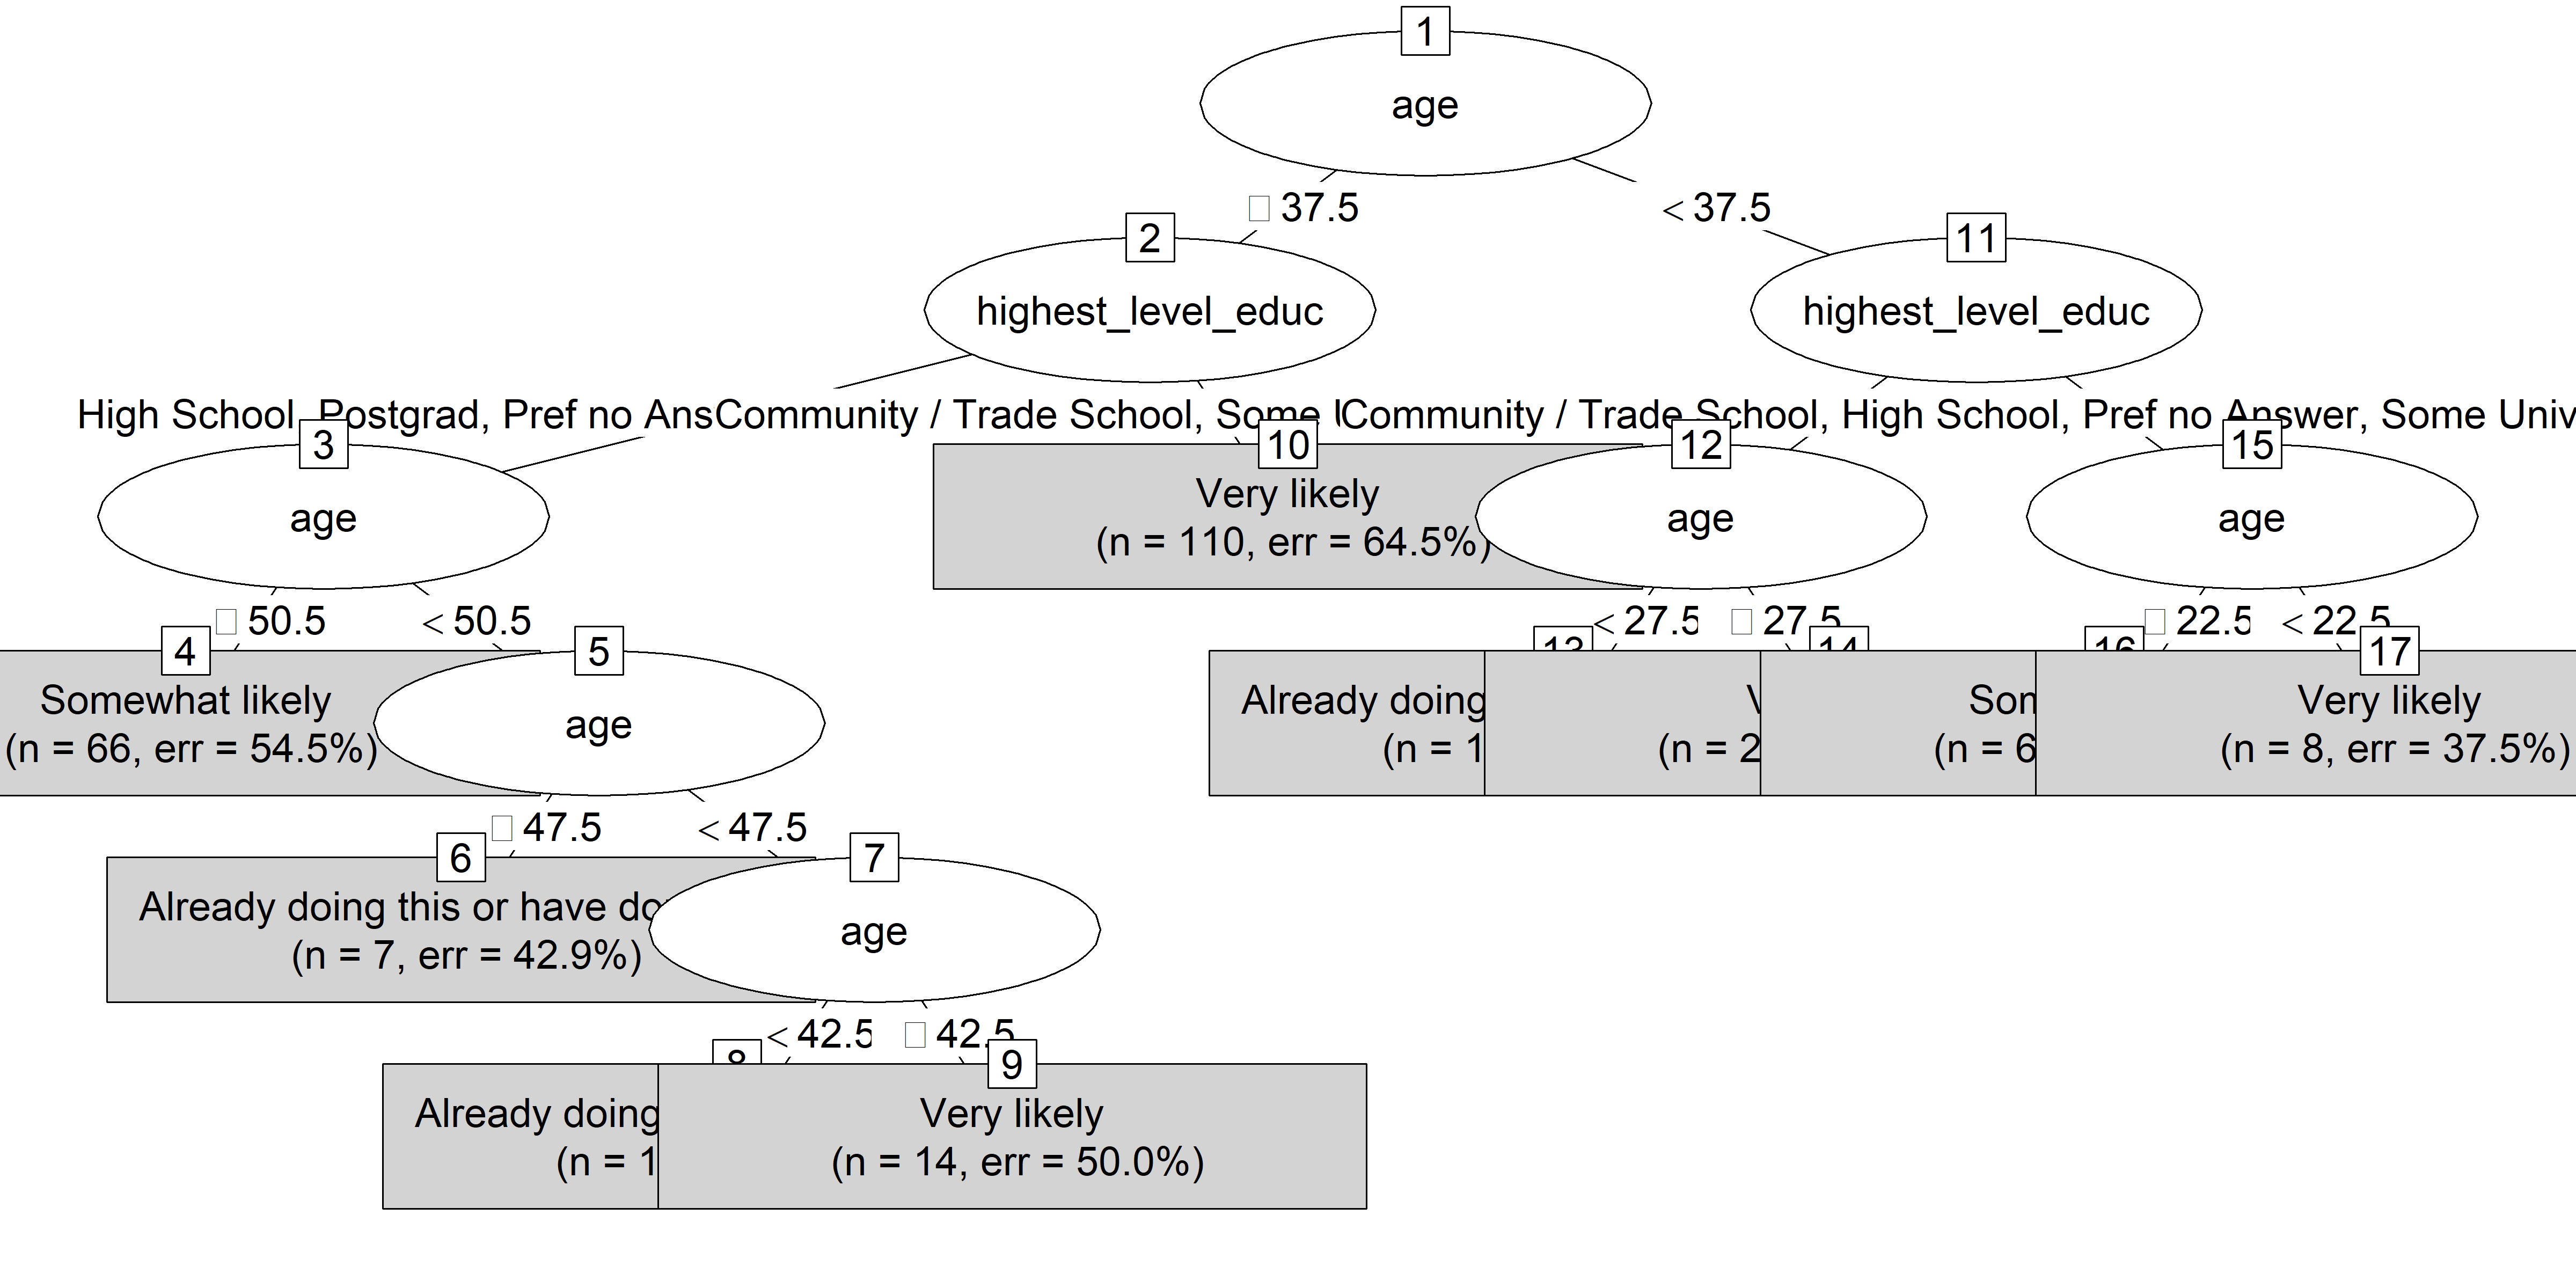
\includegraphics[width=10.67in,height=\textheight]{../models/green_product_tree.png}

}

\caption{\label{fig-thirteen}Probability tree for likelihood of
purchasing green products, predicted by age and education.}

\end{figure}%

\paragraph{Likelihood of reducing waste by repurposing used
product}\label{likelihood-of-reducing-waste-by-repurposing-used-product}

Figure~\ref{fig-fourteen} shows that age is the primary factor for waste
reduction behaviors. Younger individuals (under 35 years) are more
likely to repurpose waste, with an error rate of 57.1\%. Education
further refines the classification. Older individuals (over 35 years)
show varied likelihoods based on education, with more highly educated
individuals more likely to repurpose waste, with an error rate of 60\%.
This highlights the influence of both age and education on
waste-reduction habits.

\begin{figure}

\centering{

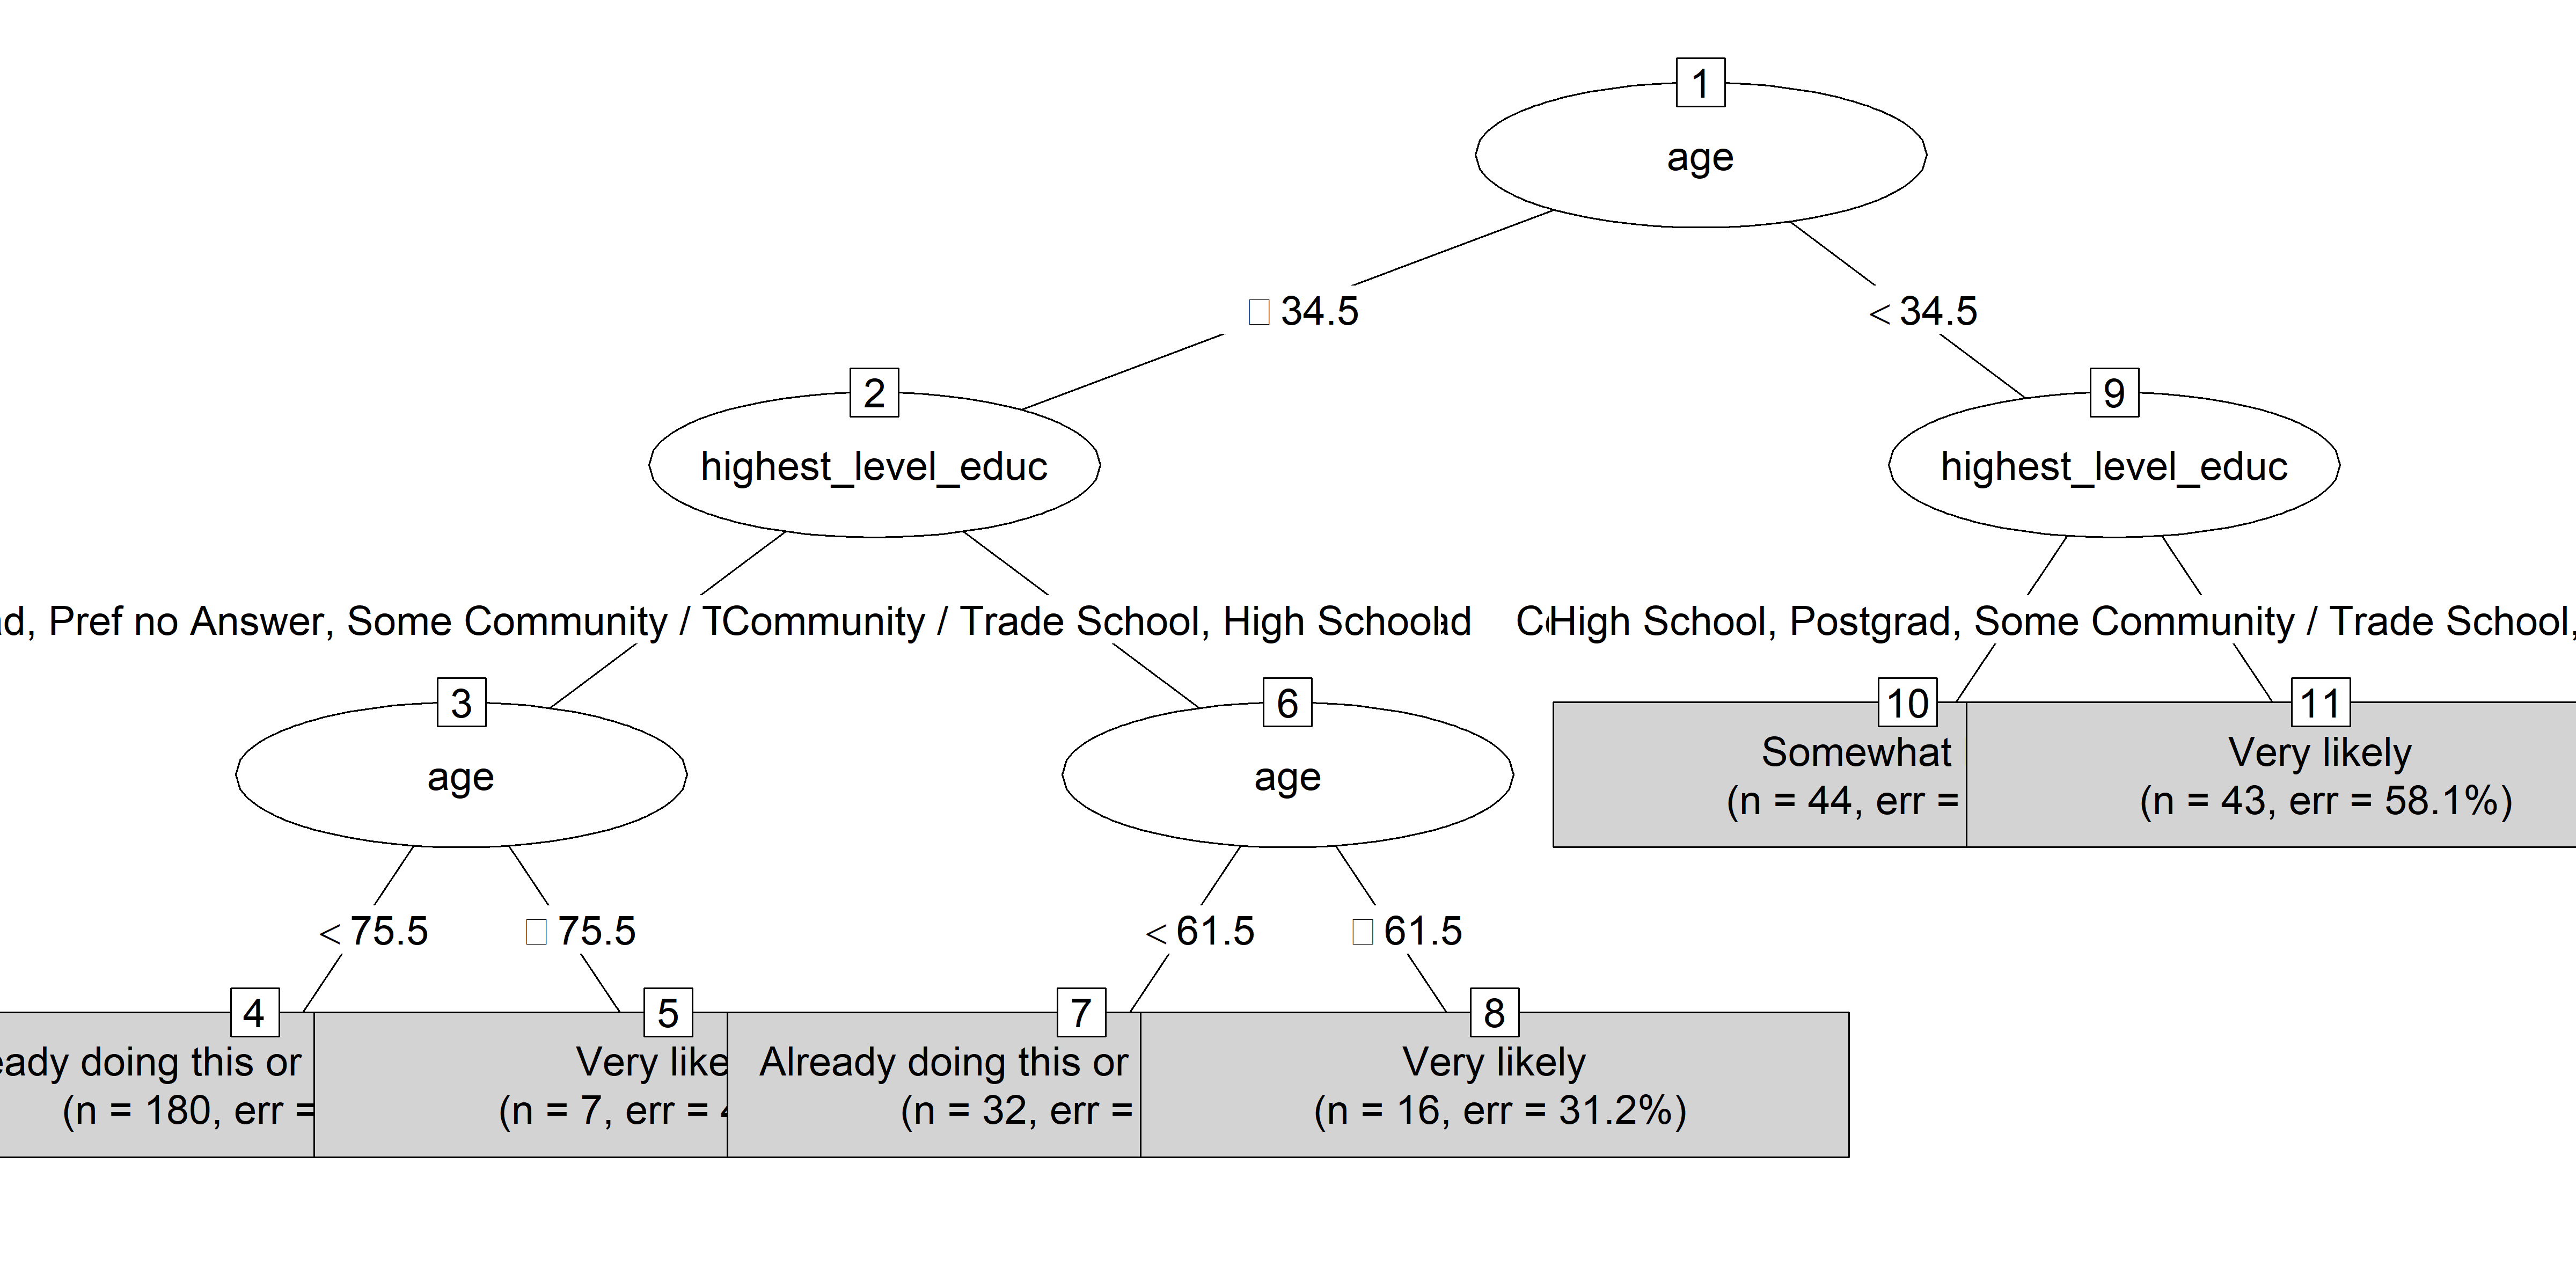
\includegraphics[width=10.67in,height=\textheight]{../models/reduce_waste_tree.png}

}

\caption{\label{fig-fourteen}Probability tree for likelihood of reducing
waste, predicted by age and education.}

\end{figure}%

\paragraph{Likelihood of sorting waste
correctly}\label{likelihood-of-sorting-waste-correctly}

Figure~\ref{fig-fifteen} identifies education as the primary factor for
sorting waste. Those with higher education (at least community/trade
school or postgraduate) are more likely to sort waste correctly, with an
error rate of 37.3\%. Age further refines the predictions for those with
lower education levels, with younger individuals under 37 years being
more likely to sort waste correctly, albeit with a higher error rate of
57.1\%. Older individuals (37 years and above) are more likely to sort
waste correctly, with an error rate of 35.3\%. The model emphasizes the
role of education in fostering proper waste-sorting behaviors, with age
providing additional nuance.

\begin{figure}

\centering{

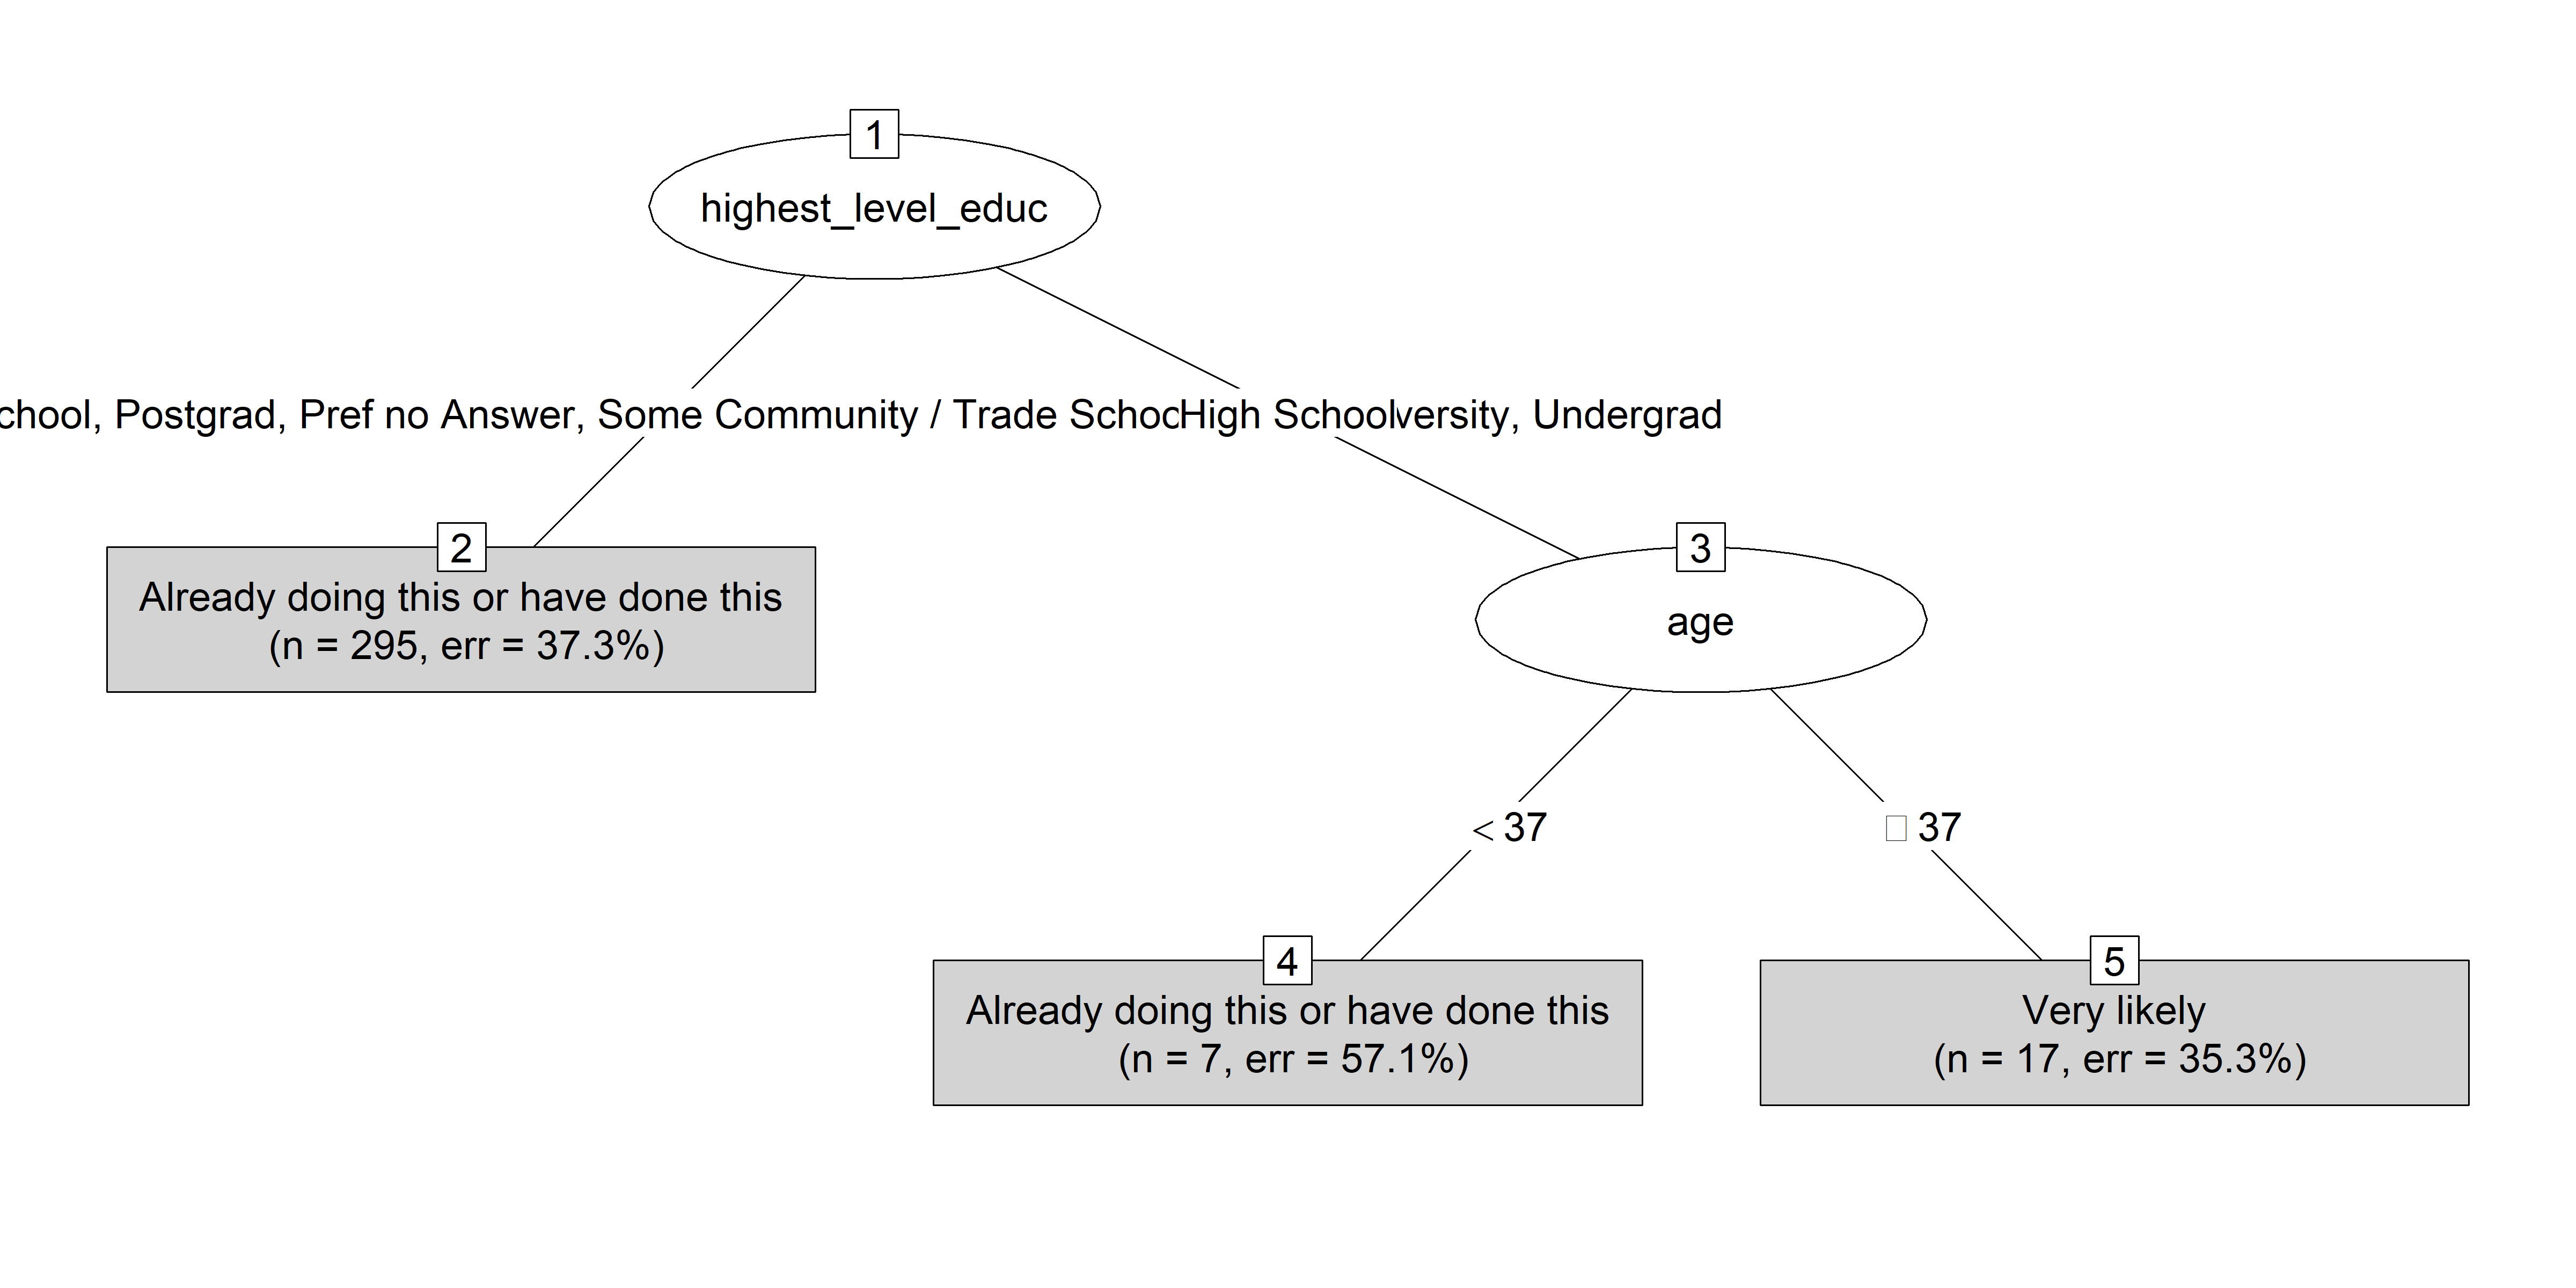
\includegraphics[width=10.67in,height=\textheight]{../models/sort_waste_tree.png}

}

\caption{\label{fig-fifteen}Probability tree for likelihood of sorting
waste correctly, predicted by age and education.}

\end{figure}%

\subsubsection{Home and Lifestyle
Changes}\label{home-and-lifestyle-changes}

\paragraph{Likelihood of making home
improvements}\label{likelihood-of-making-home-improvements}

Figure~\ref{fig-sixteen} shows that age is the key predictor for home
improvement behavior. Individuals aged 36 years and older are
predominantly classified as ``Already doing this or have done this,''
with an error rate of 59.6\%. For younger individuals (under 36),
education plays a role: those with higher educational attainment
(``Community/Trade School,'' ``Some University,'' or ``Postgraduate'')
are ``Very likely'' to make home improvements, with an error rate of
55\%. Conversely, individuals with lower education levels are classified
as ``Somewhat likely,'' with a higher error rate of 67.4\%. This model
highlights how age and education interact to influence home improvement
decisions.

\begin{figure}

\centering{

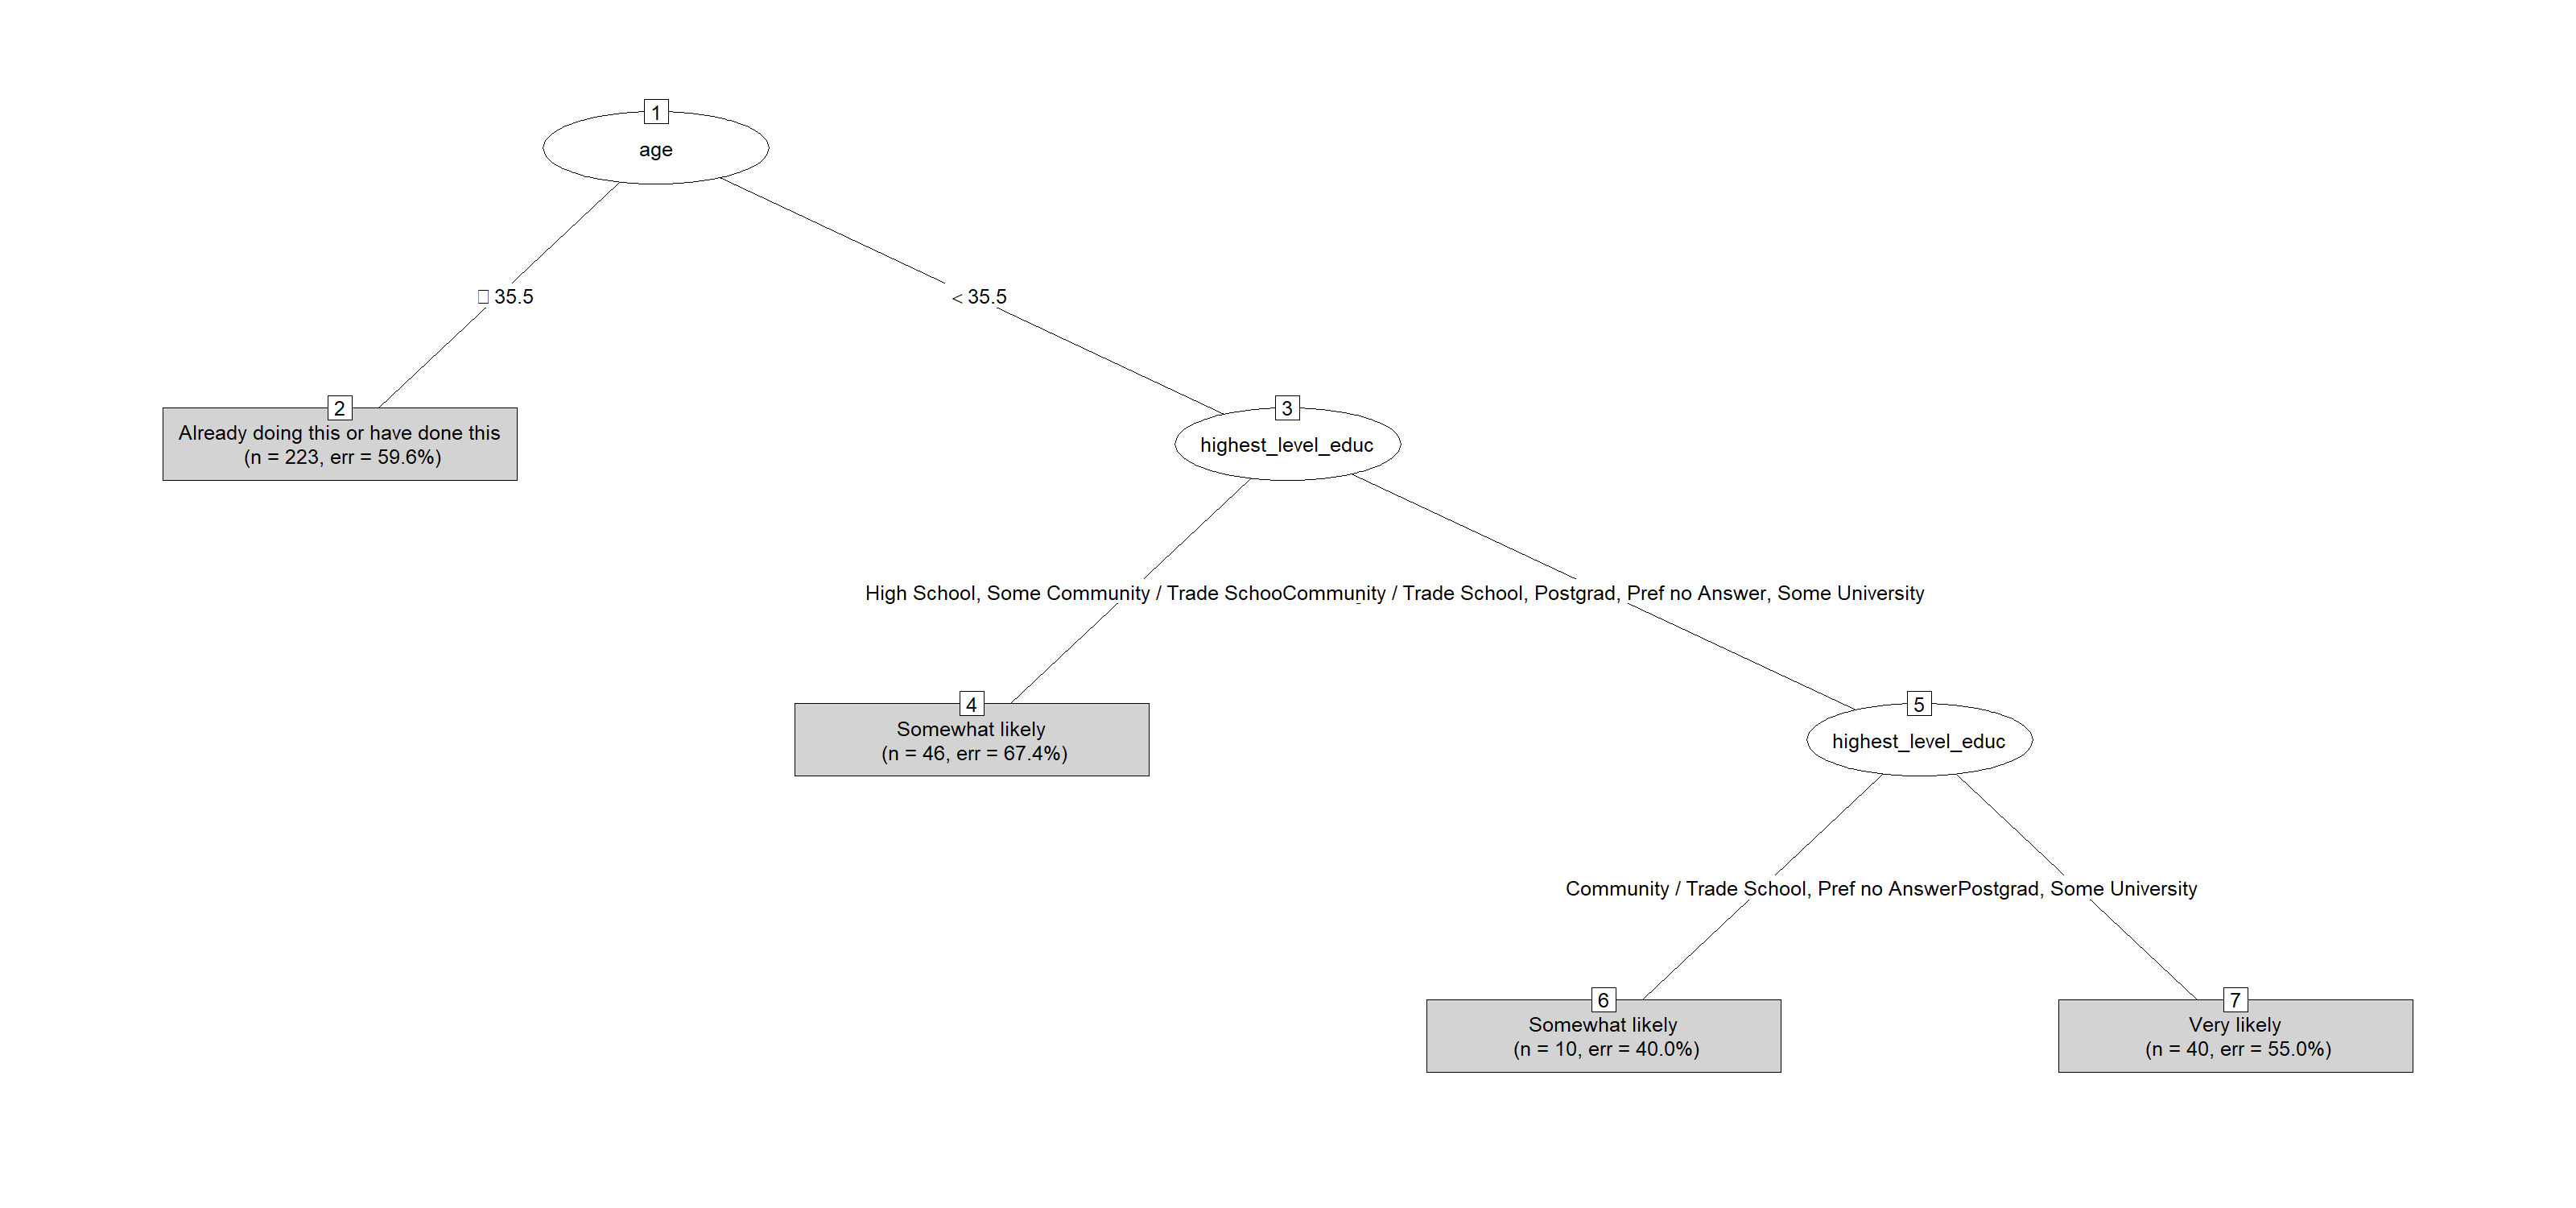
\includegraphics[width=10.67in,height=\textheight]{../models/home_improvement_tree.png}

}

\caption{\label{fig-sixteen}Probability tree for likelihood of making
home improvements predicted by age and education.}

\end{figure}%

\paragraph{Likelihood of adopting meat
alternatives}\label{likelihood-of-adopting-meat-alternatives}

Figure~\ref{fig-seventeen} demonstrates that age is the primary factor
for adopting meat alternatives. Younger individuals (under 35 years) are
more likely to adopt meat alternatives, with an error rate of 44\%. For
individuals aged 35 years or older, education becomes a key predictor.
Those with community/trade school, undergraduate, or postgraduate
education are more likely to adopt meat alternatives, with varying error
rates, including ``Somewhat unlikely'' for younger individuals at
62.9\%. This model highlights how age and education together shape
dietary choices.

\begin{figure}

\centering{

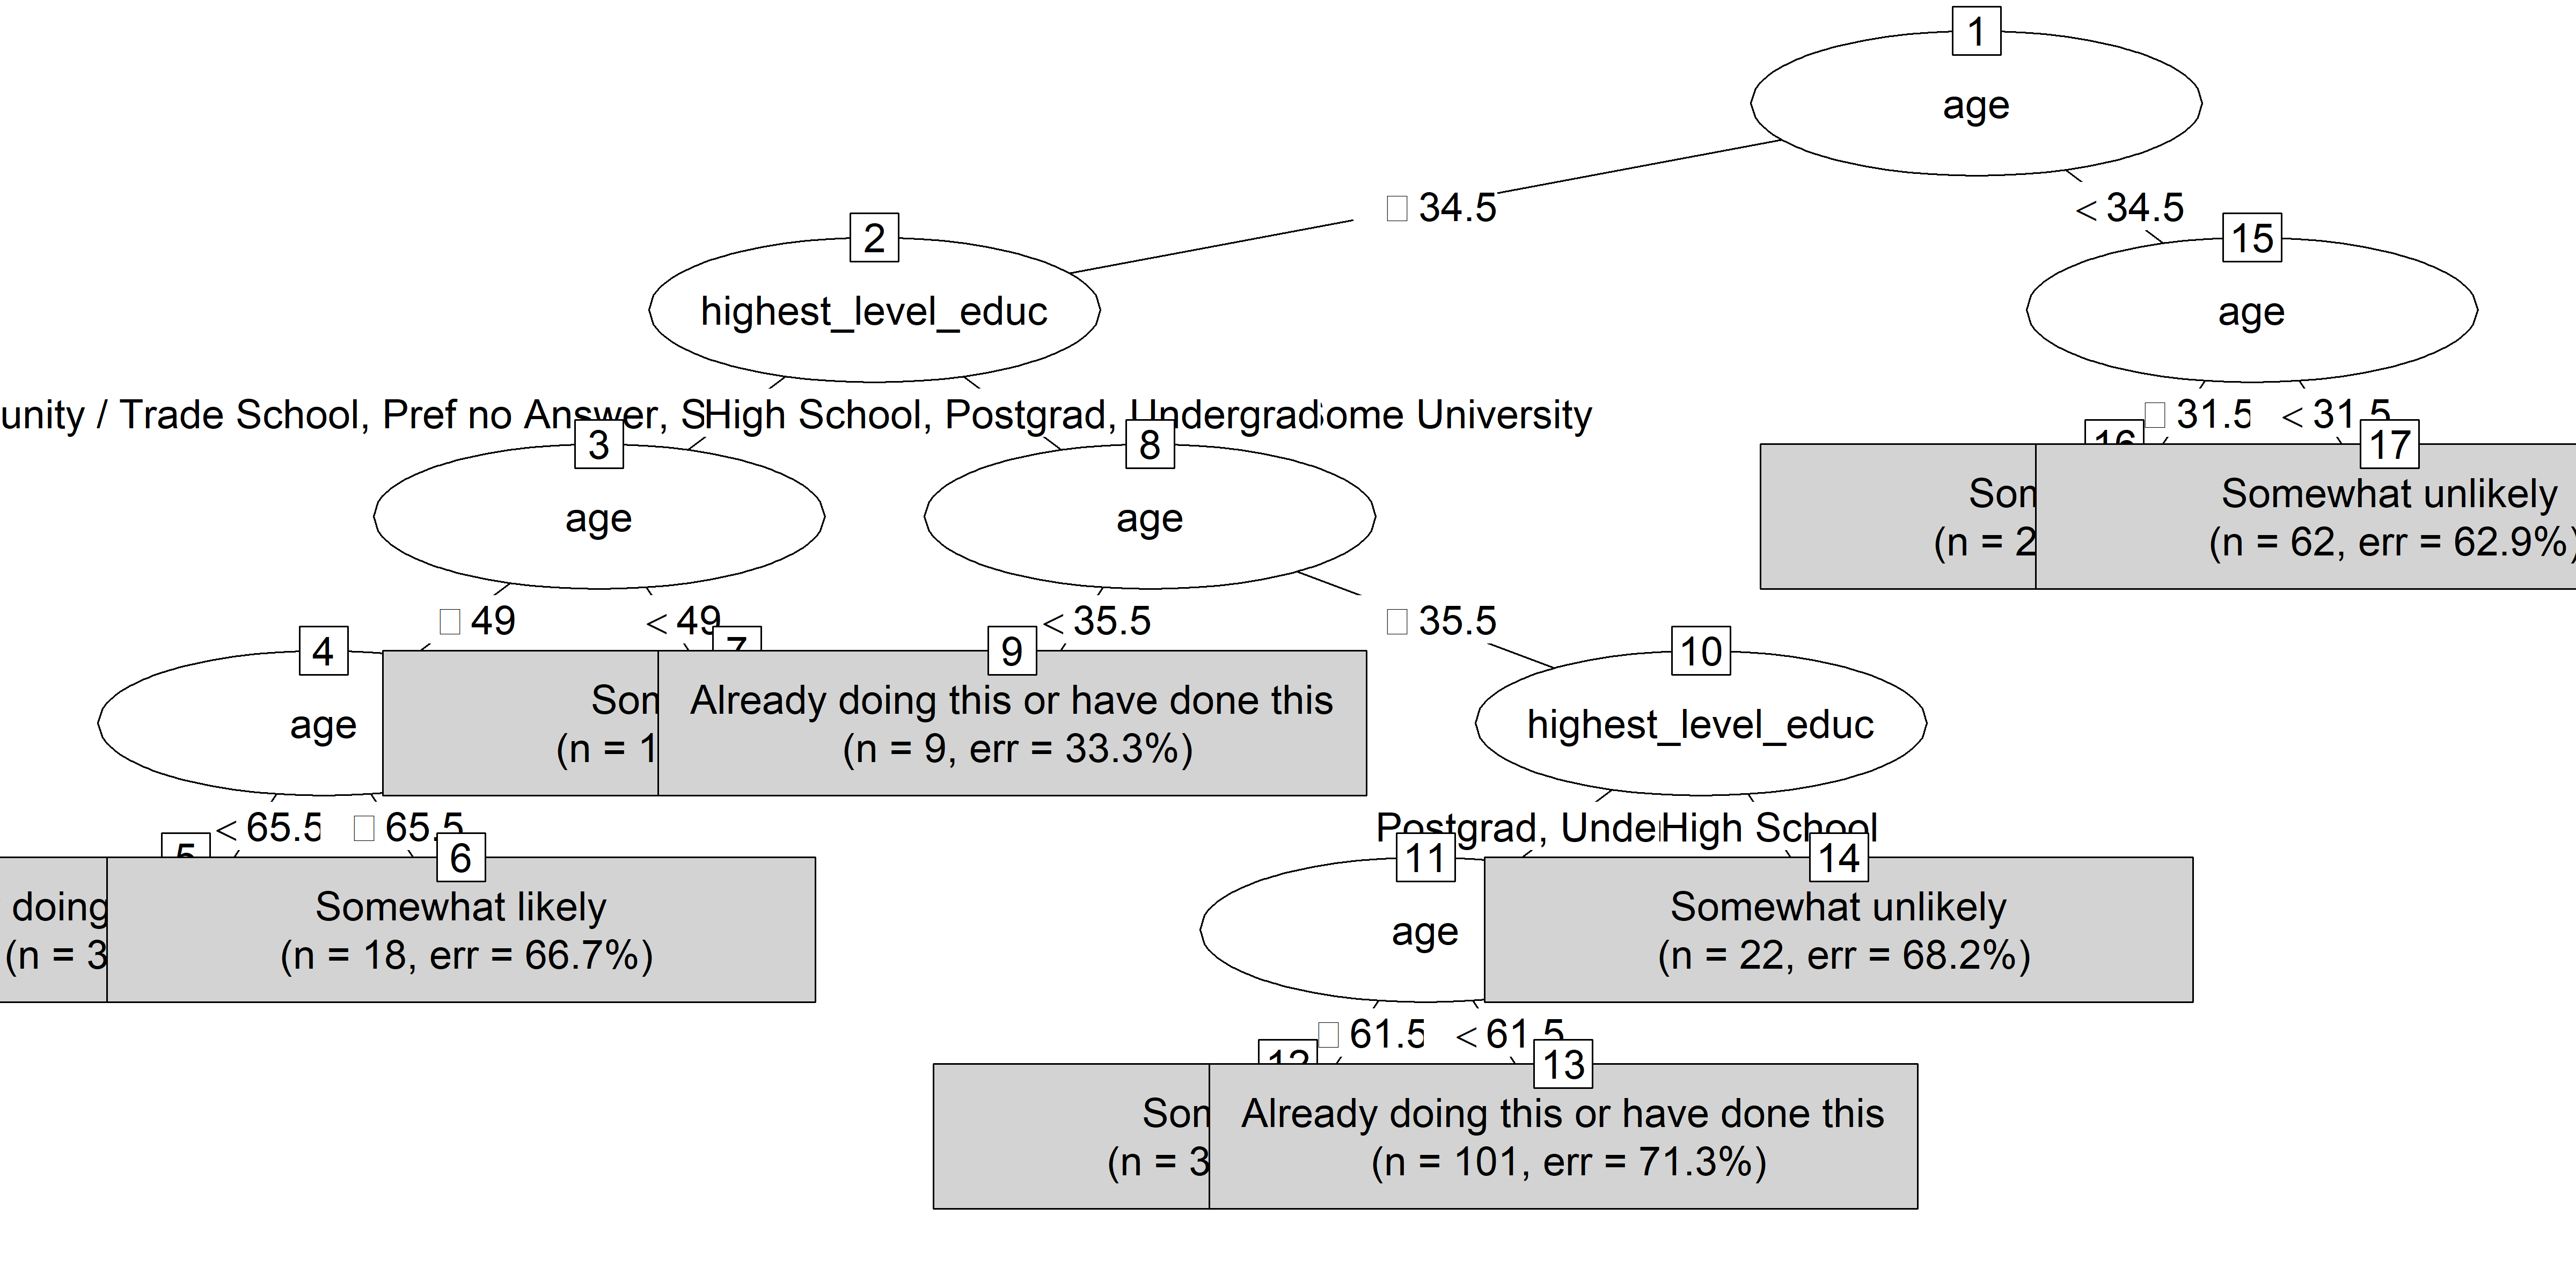
\includegraphics[width=10.67in,height=\textheight]{../models/protein_alternative_tree.png}

}

\caption{\label{fig-seventeen}Probability tree for likelihood of
adopting meat alternatives, predicted by age and education.}

\end{figure}%

\paragraph{Likelihood of reducing hydro
usage}\label{likelihood-of-reducing-hydro-usage}

Figure~\ref{fig-eighteen} reveals that age is the primary predictor
influencing hydro usage reduction. Younger individuals (under 35 years)
are ``Very likely'' to reduce hydro usage, with an error rate of 60.9\%.
Older individuals (35 years and above) are further split by education
and age, with those over 64 years also ``Very likely'' to engage in
hydro conservation, with a lower error rate of 37.5\%. Middle-aged
individuals (35--64 years) with higher education are either ``Already
doing this or have done this'' (error rate 56.3\%) or ``Somewhat
likely'' (error rate 50.0\%). This model underscores the combined role
of age and education in promoting energy-saving behaviors.

\begin{figure}

\centering{

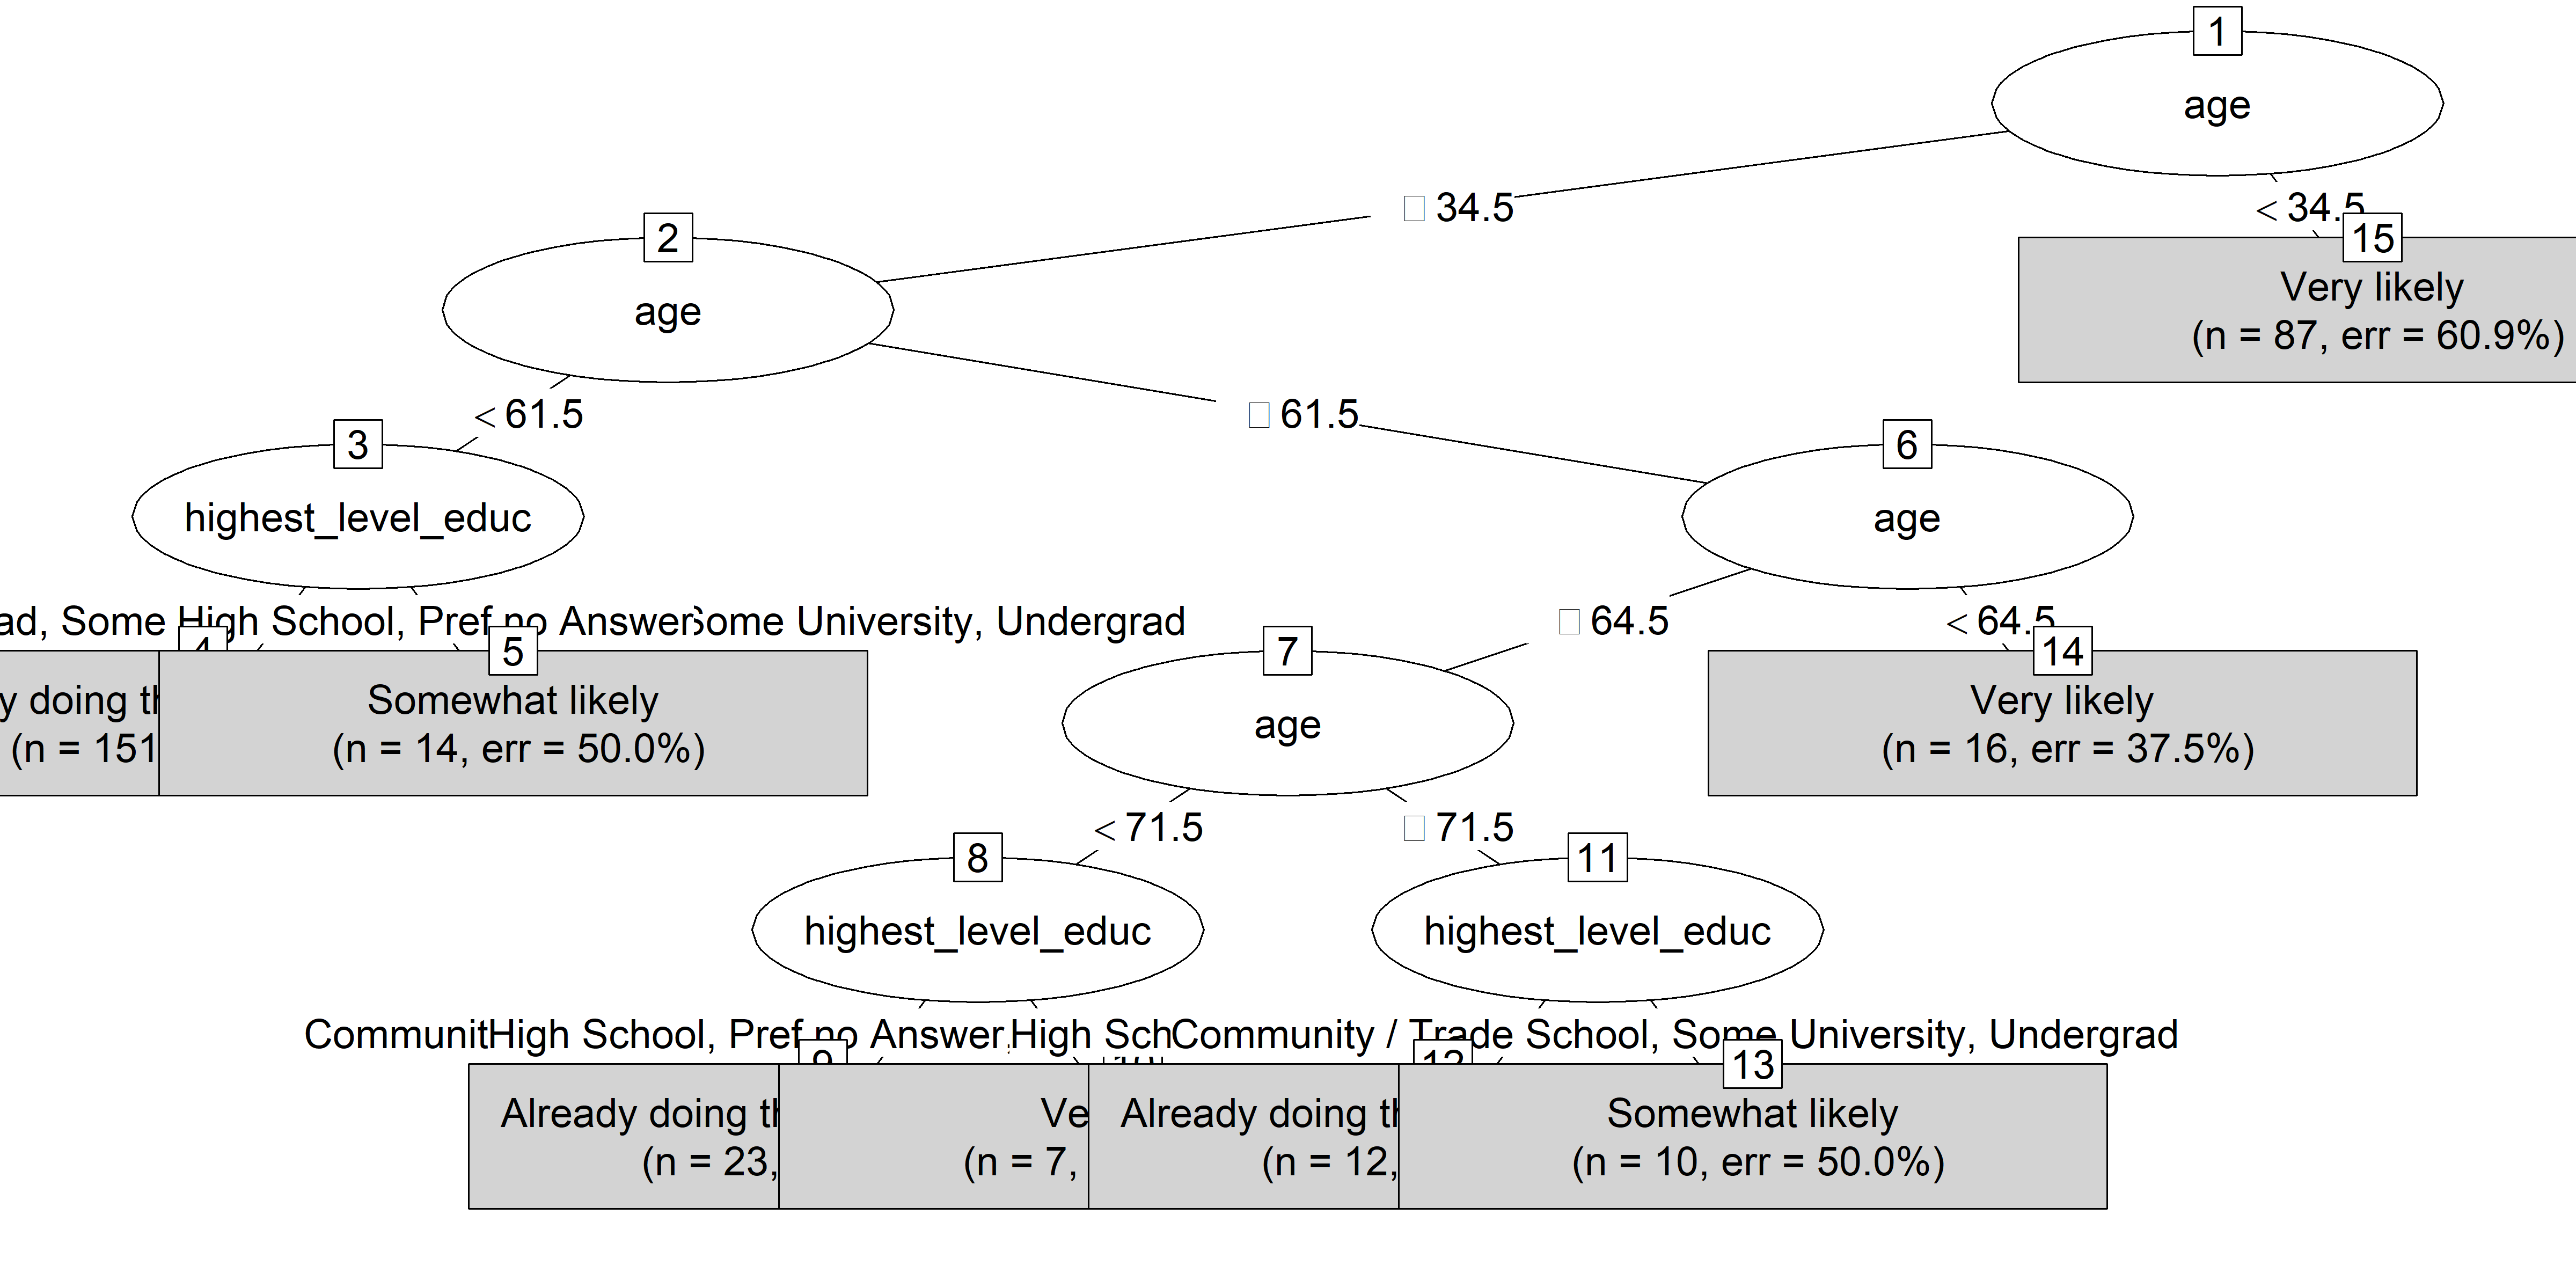
\includegraphics[width=10.67in,height=\textheight]{../models/reduce_hydro_tree.png}

}

\caption{\label{fig-eighteen}Probability tree for likelihood of reducing
hydro usage, predicted by age and education.}

\end{figure}%

\subsection{Results}\label{sec-results}

\subsection{Model Summary Table}\label{model-summary-table}

\textbf{?@fig-nineteen} presents the accuracy of models predicting
climate-friendly actions based on age and education. A threshold emerges
from the data: models with accuracy above 50\% are considered reliable,
while those below require careful interpretation. Sorting waste
correctly, with an accuracy of 59\%, is the most reliable prediction,
indicating a stronger association between demographic factors and this
behavior. Models like home improvements (33\%) offer limited predictive
value but remain somewhat informative. In contrast, actions such as
adopting meat alternatives (25\%) or choosing electric or hybrid
vehicles (25\%) approach random chance, making their predictions less
reliable for drawing meaningful conclusions.

\subsection{Likelihood taking action by
age}\label{likelihood-taking-action-by-age}

Figure~\ref{fig-twenty} shows the relationship between age and the
likelihood of engaging in various climate-related actions. The x-axis
represents the age groups, and the y-axis indicates the percentage of
respondents reporting different likelihood levels, from ``Already doing
this'' to ``Very unlikely''.

\subsubsection{Transportation Actions}\label{transportation-actions-1}

In the category of transportation actions, the results reveal that for
electric and hybrid vehicles, there is little difference between age
groups in terms of the likelihood of adopting this behavior, but older
individuals, particularly those aged 65+, are more likely to report
being ``very unlikely'' to do so. For minimizing car use, individuals
across all age groups report similar levels of engagement, with
relatively consistent percentages already minimizing their car use.
However, older individuals, particularly those in the 45-54 and 65+ age
groups, are more likely to report being ``very unlikely'' to minimize
car use. For walking or cycling short distances, the trend shows that
all age groups, except for those aged 25-34, report similar levels of
engagement, with a slight decrease in adoption among the 25-34 age
group. Conversely, older individuals, especially those aged 65+, are
more likely to report being ``very unlikely'' to engage in walking or
cycling for short distances.

\subsubsection{Waste and Product
Actions}\label{waste-and-product-actions-1}

When examining purchasing green products, individuals aged 35 and older
report higher engagement in this action, with many already purchasing
green products or expressing a strong likelihood of doing so. Notably,
those aged 45 and above are the least likely to adopt this behavior,
with a significant percentage indicating they are ``very unlikely'' to
do so. For reducing waste, older age groups show higher levels of
engagement, with individuals aged 35 and above reporting the highest
rates of already taking this action. The 45-54 age group, however, is
the least likely to engage in this behavior. Sorting waste correctly is
overwhelmingly supported by all age groups, with at least 75\% in each
category already doing or being very likely to take action. The
incidence of individuals reporting being ``very unlikely'' to sort waste
correctly is minimal across all age groups.

\subsubsection{Home and Lifestyle
Changes}\label{home-and-lifestyle-changes-1}

For making home improvements aimed at increasing energy efficiency,
middle-aged individuals (35-54) are the most likely to report having
already made improvements or being very likely to do so. Across all age
groups, at least half of the respondents are already engaged in or very
likely to engage in energy-efficient home improvements, though younger
individuals (15-24) are less likely to take this action. Regarding
adopting meat alternatives, younger individuals, particularly those aged
15-24, are the least likely to reduce meat consumption with plant-based
alternatives. In contrast, individuals aged 35 and older show higher
levels of adoption or strong intention to adopt this behavior. Lastly,
for reducing hydro usage, there is a clear increase in the likelihood of
engagement with increasing age. Older individuals, particularly those
aged 65+, are more likely to report already reducing their hydro usage
or being very likely to do so, though the 65+ age group also reports the
highest percentage of being ``very unlikely'' to reduce hydro usage.

\begin{figure}

\centering{

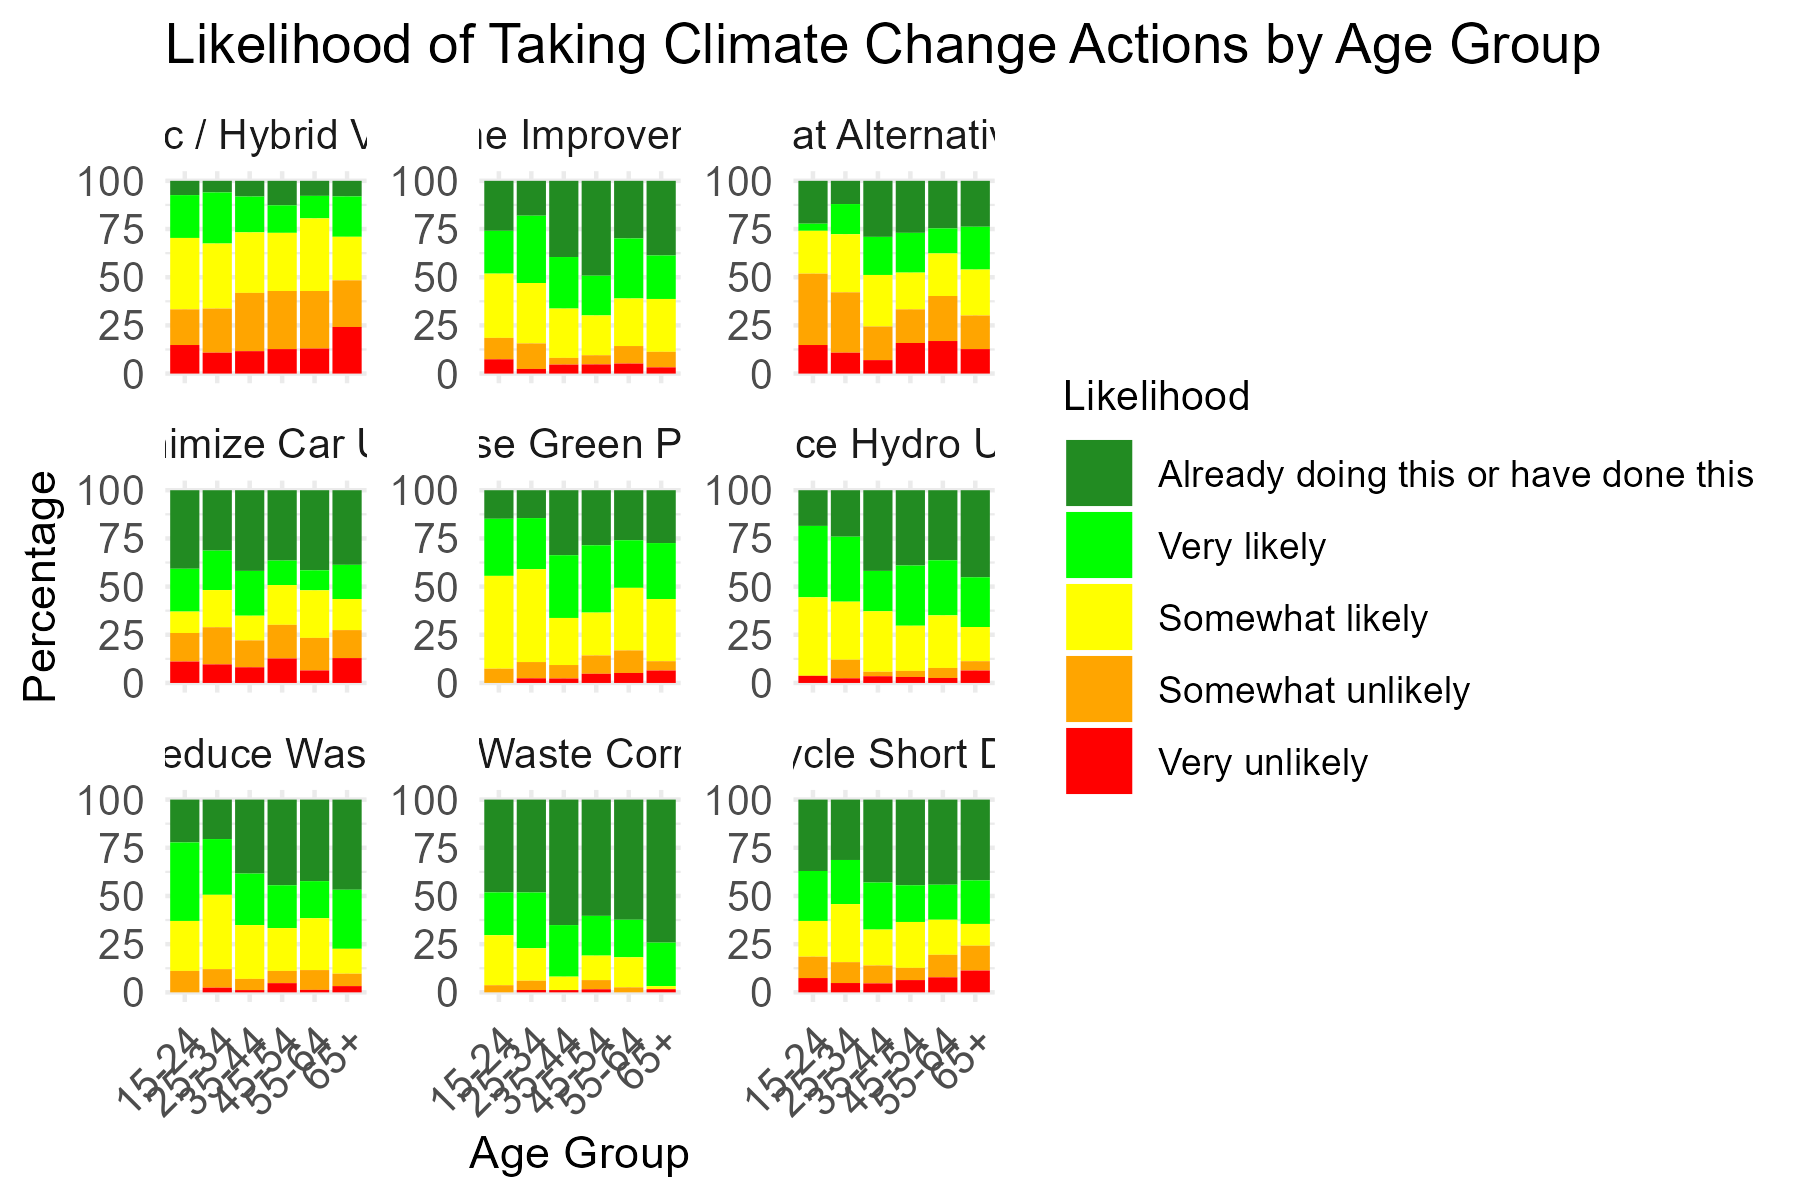
\includegraphics[width=9in,height=\textheight]{../data/03-figures_data/likelihood_age_plot.png}

}

\caption{\label{fig-twenty}Likelihood of Taking Climate Change Actions
by Age Group. The stacked bar chart illustrates the percentage of
respondents across six age groups (15-24, 25-34, 35-44, 45-54, 55-64,
65+) in terms of their self-reported likelihood to engage in nine
distinct climate-related actions. Each color represents a different
level of likelihood, from ``Already doing this or have done this'' to
``Very unlikely.'' The black dashed trend line highlights how the
likelihood of action changes across age groups, providing insights into
generational differences in climate-related behavior.}

\end{figure}%

\subsection{Likelihood taking action by
education}\label{likelihood-taking-action-by-education}

Figure~\ref{fig-twenty-one} displays how the likelihood of engaging in
climate-friendly actions varies by educational attainment. The x-axis
represents the proportion of respondents in each education category,
while the y-axis lists the educational levels, from low to high
educational attainment. Each action is shown across separate facets,
revealing how education level correlates with engagement in each
behavior.

\subsubsection{Transportation Actions}\label{transportation-actions-2}

In the category of transportation actions, the likelihood of adopting
electric or hybrid vehicles does not significantly vary across age
groups, but older individuals, particularly those aged 65+, are more
likely to report being ``very unlikely'' to adopt this action. When
considering minimizing car use, responses show relatively consistent
engagement across all age groups, with similar percentages already
engaging in this action. However, older age groups, particularly those
aged 45-54 and 65+, are more likely to report being ``very unlikely'' to
minimize their car use. For walking or cycling shorter distances, the
trend is fairly consistent across age groups, with all groups showing
similar levels of adoption, except for those aged 25-34, who report
slightly lower engagement. Older age groups, particularly individuals
aged 65+, are also more likely to report being ``very unlikely'' to
engage in walking or cycling for short distances.

\subsubsection{Waste and Product
Actions}\label{waste-and-product-actions-2}

Regarding purchasing green products, individuals aged 35 and older show
higher levels of engagement, with a significant proportion already
purchasing or expressing strong intentions to do so. Conversely,
individuals aged 45 and older exhibit lower likelihoods, with a higher
percentage reporting being ``very unlikely'' to adopt this behavior. For
reducing waste, older age groups (35 and above) are more likely to have
already taken action or express high intentions to do so. However, the
45-54 age group stands out as the least likely to engage in this action.
Sorting waste correctly is a behavior that is overwhelmingly practiced
across all age groups, with at least 75\% of individuals from every age
category reporting that they are already doing it or are very likely to
do so. The percentage of individuals reporting being ``very unlikely''
to sort waste correctly is minimal across all age groups.

\subsubsection{Home and Lifestyle
Changes}\label{home-and-lifestyle-changes-2}

For making home improvements to increase energy efficiency, individuals
in the 35-54 age range are the most likely to report having already made
improvements or being very likely to do so. In general, at least half of
the sample across all age groups reports that they are already engaged
in or very likely to make energy-efficient home improvements, although
younger individuals (15-24) are less likely to take this action. When it
comes to adopting meat alternatives, individuals aged 35 and above are
more likely to reduce meat consumption with plant-based alternatives,
while those aged 15-24 are the least likely to engage in this behavior.
For reducing hydro usage, older age groups, particularly those aged 65+,
report the highest rates of already engaging in or being very likely to
engage in this action. However, the 65+ age group also reports the
highest percentage of being ``very unlikely'' to reduce hydro usage.

\begin{figure}

\centering{

\captionsetup{labelsep=none}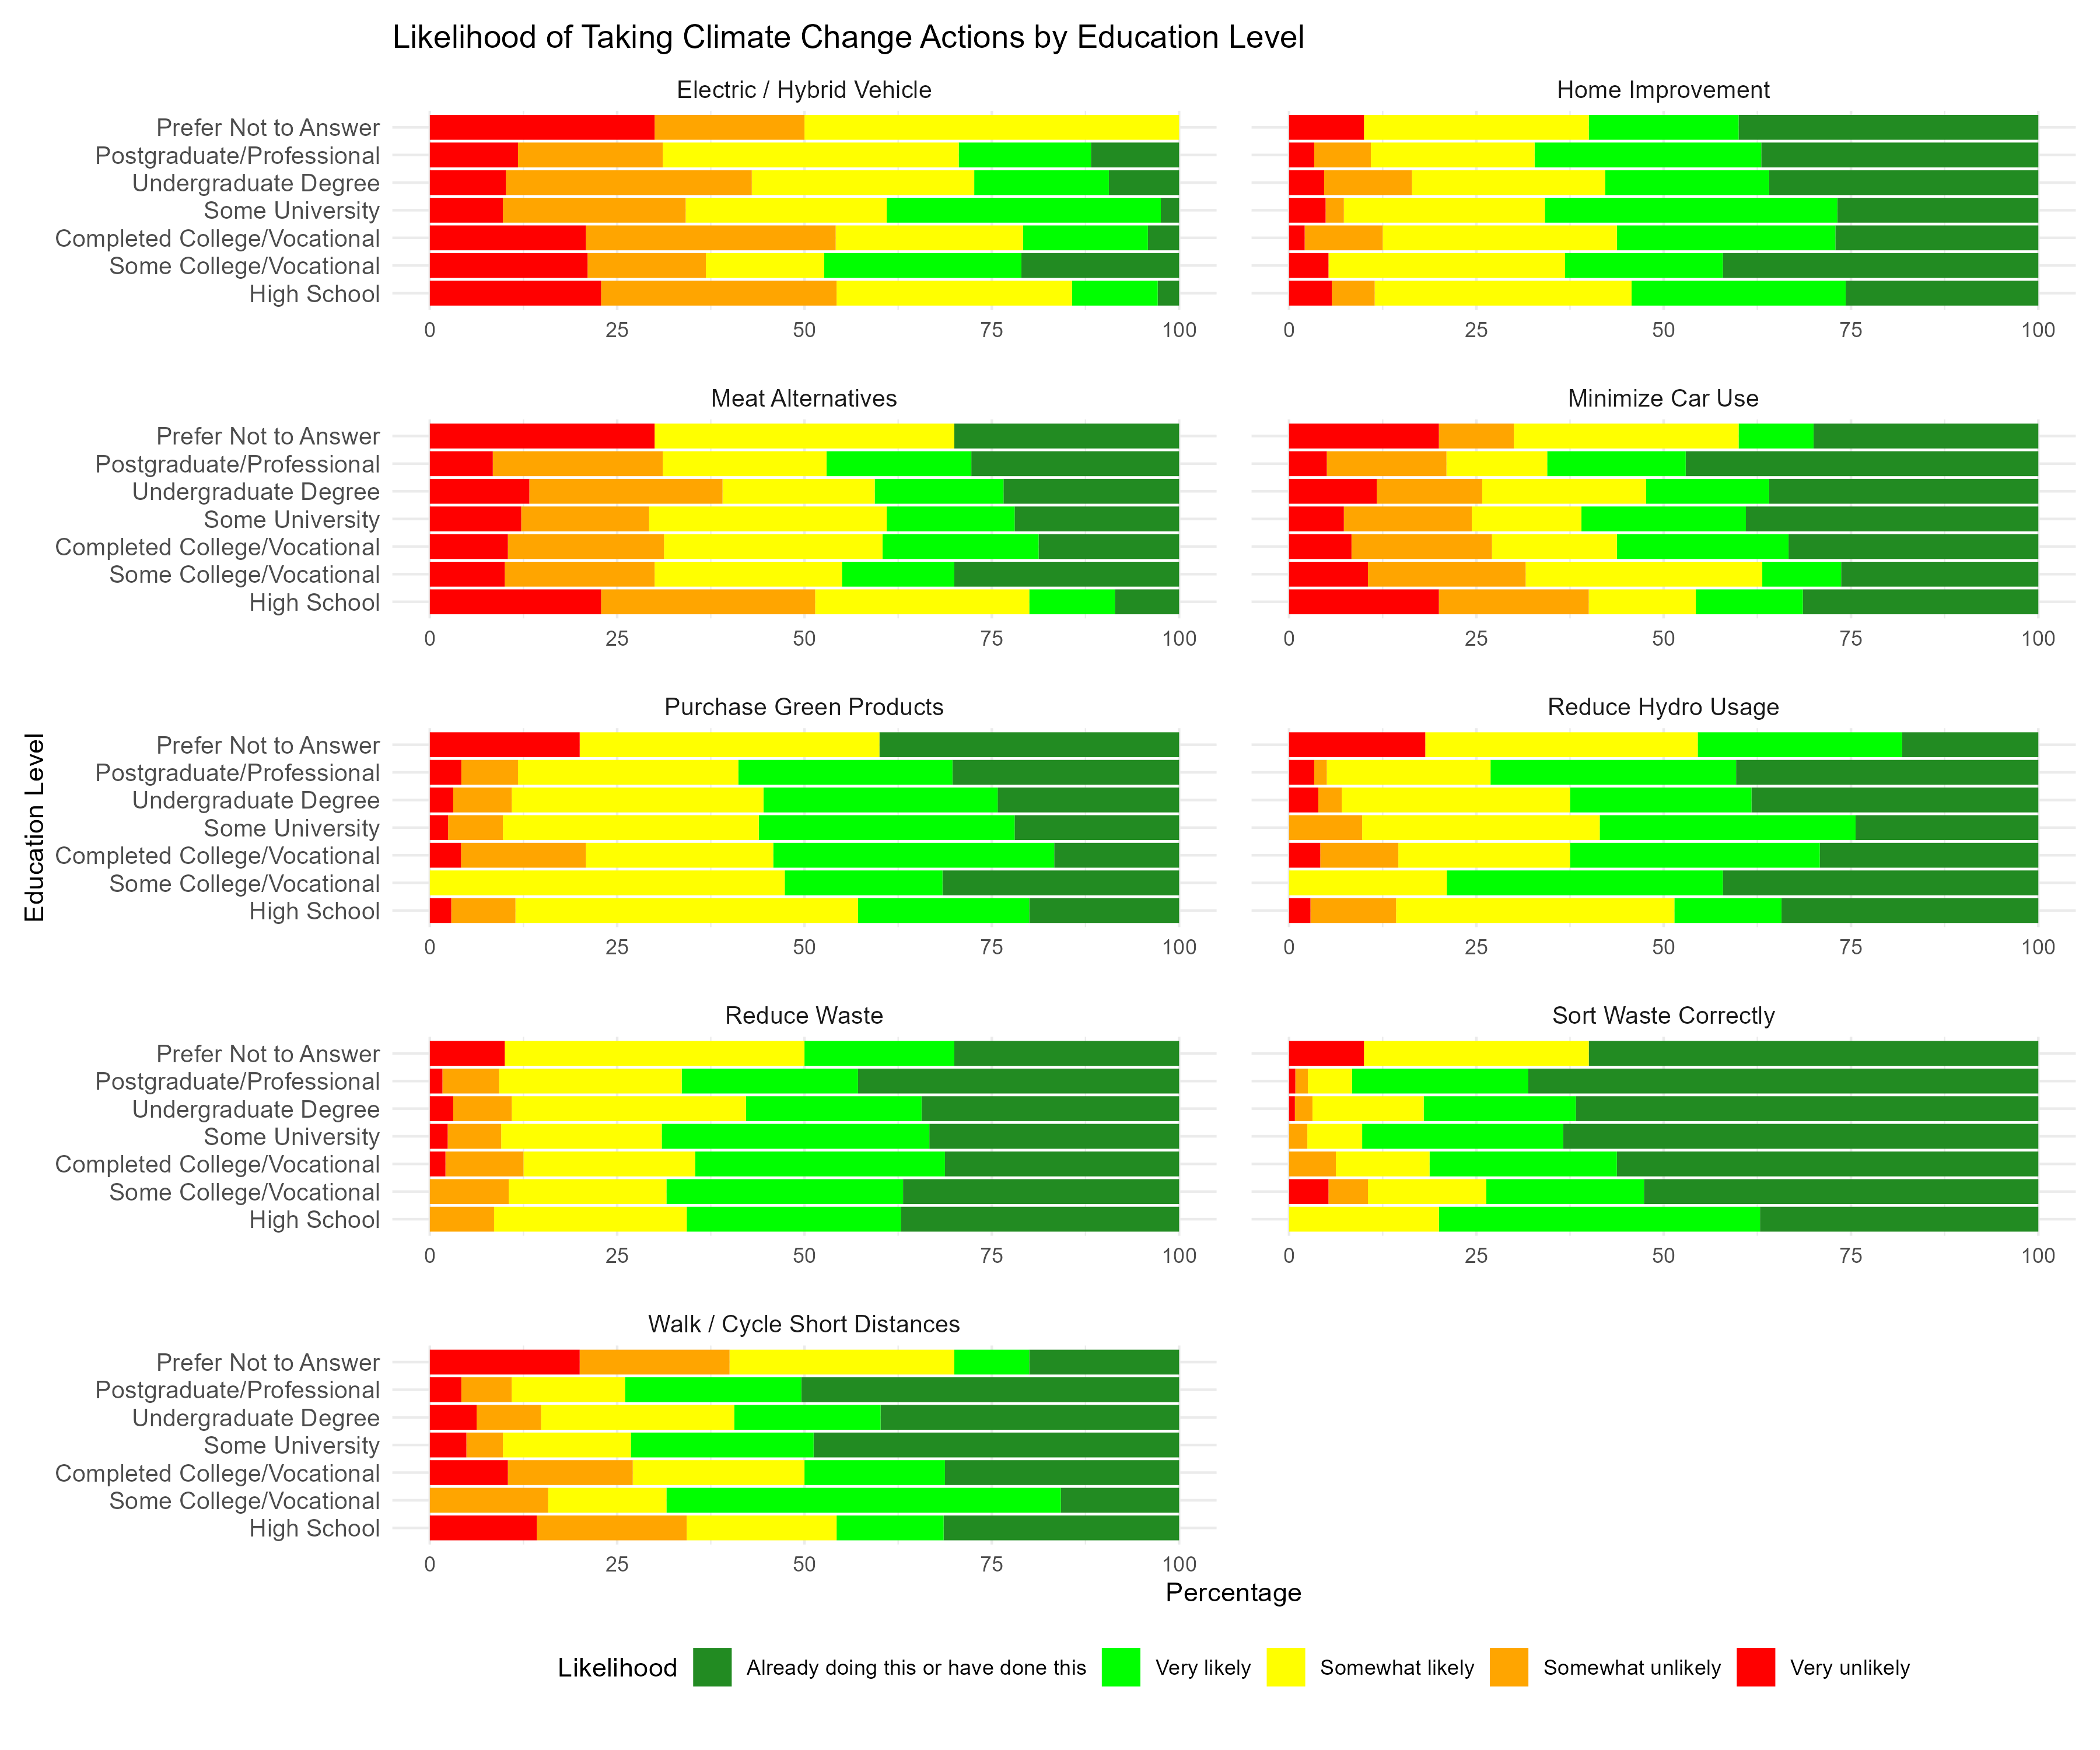
\includegraphics[width=9in,height=\textheight]{../data/03-figures_data/likelihood_education_plot.png}

}

\caption{\label{fig-twenty-one}}

\end{figure}%

\subsection{Discussion}\label{sec-discussion}

\subsection{Overview of Climate Change
Perspectives}\label{overview-of-climate-change-perspectives}

This paper explored how various demographic factors---such as age,
education, and climate change knowledge---affect individuals' engagement
in climate-friendly behaviors. Through a comprehensive analysis of
survey data from 2018 and 2021, we uncovered surprising patterns and
deeper insights into the influences that drive people to adopt more
sustainable actions. By investigating the interplay of these factors, we
aimed to shed light on how societal changes, particularly in the context
of climate action, reflect evolving values and behaviors.

\subsection{What We Learn About the
World}\label{what-we-learn-about-the-world}

\subsection{Age and Climate-Friendly Behaviors}\label{sec-first-point}

Initially, we anticipated that younger individuals would lead the way in
adopting climate-friendly actions. While younger people did excel in
behaviors like walking or cycling and adopting meat alternatives, the
older demographic demonstrated more significant commitment to long-term
sustainable actions, such as making energy-efficient home improvements
and reducing waste. This unexpected finding revealed that age influences
sustainability in complex ways: younger people may embrace immediate,
accessible actions, while older individuals engage in more
transformative, lasting efforts. This highlights that climate action is
a multi-generational effort, with each age group contributing in its own
way.

\subsection{The Role of Education in Sustainable
Actions}\label{sec-second-point}

We initially hypothesized that higher education levels would lead to
greater engagement in climate-friendly behaviors, and the data largely
supported this. Individuals with higher educational attainment were more
likely to adopt green products and engage in waste reduction. However,
some behaviors, such as reducing meat consumption, were less influenced
by education and more affected by lifestyle preferences and cultural
norms. Education acts as a strong catalyst for sustainability, but it
works in conjunction with other factors, such as age and socio-economic
status, to shape climate action. This reminds us that while education is
a powerful tool for promoting sustainable behaviors, it is not the only
factor at play.

\subsection{The Influence of Climate Change
Knowledge}\label{sec-third-point}

To effectively encourage individuals to take climate action, it's
crucial to consider the most popular and impactful methods of
communication. Based on the findings from both 2018 and 2021, the most
common methods for engaging individuals in climate-friendly behavior are
ad campaigns, city newsletters/emails, and the official torontoca
website. However, there has been a notable shift towards more diverse,
digitally-focused strategies. Social media platforms, particularly
Instagram and Twitter, have seen a significant increase in usage since
2018. These platforms allow for more dynamic, engaging, and personalized
communication, which can be particularly effective for reaching younger
demographics. Smith and Brown (Smith and Brown 2023) discuss how digital
media can drive climate action by engaging youth through interactive and
tailored content, offering an effective way to reach younger individuals
who are more digitally engaged. Traditional methods, such as newsletters
and brochures, continue to play a role but are becoming less dominant.
To maximize engagement, a multi-channel approach that blends digital and
traditional communication methods will likely resonate best with the
broadest audience, particularly when targeting specific age groups and
education levels.

\subsection{Weaknesses of the Study}\label{weaknesses-of-the-study}

One limitation of this study is its reliance on self-reported survey
data, which can be biased by social desirability or recall errors.
Respondents may overestimate their commitment to sustainability or
exaggerate their behaviors to align with societal expectations.
Additionally, the use of summary data instead of individual-level data
constrained our ability to explore complex interactions between
socio-economic factors and climate behaviors. Future studies that
utilize individual-level data and more objective measures, such as
energy consumption records, would provide a clearer picture of the
drivers behind climate action.

Survey data also presents challenges related to non-response bias, where
certain demographic groups may be underrepresented, skewing results.
Additionally, the framing of questions can influence responses, which
could introduce variability in the data. The inability to verify
self-reported behaviors further limits the reliability of the
conclusions drawn from such datasets. Despite these challenges, surveys
remain a valuable tool for understanding attitudes and behaviors, but
their findings should be interpreted with caution and complemented with
more direct forms of data collection.

\subsection{Future Directions}\label{future-directions}

To build on these findings, future research should focus on identifying
the barriers that prevent certain groups from engaging in
climate-friendly actions. By examining factors such as income, access to
resources, and perceived obstacles to sustainability, we can tailor
interventions to address specific needs. For example, financial
incentives or public infrastructure improvements could make sustainable
behaviors more accessible and feasible for low-income individuals.
Longitudinal studies will also help track how climate awareness
influences sustained behavioral changes over time, offering insights
into the effectiveness of educational and policy interventions.

Lastly, incorporating objective data such as energy usage and
transportation patterns could complement self-reported behaviors and
validate the findings. This integrated approach would provide a more
comprehensive understanding of how demographic factors shape sustainable
actions, ultimately informing more effective climate policies.

\section{Conclusion}\label{sec-conclusion}

This paper examined how age, education, and climate-friendly behaviors
intersect, revealing that while younger individuals engage in more
immediate actions like walking and adopting meat alternatives, older
individuals tend to adopt long-term sustainable practices such as
energy-efficient home improvements and waste reduction. Education plays
a significant role in fostering sustainable behavior, though it works
alongside other factors like income and lifestyle. The rise of digital
media, especially social platforms, is crucial for engaging younger
generations in climate action. Despite challenges such as biases in
self-reported data, the study highlights the need for targeted
strategies and multi-channel communication to drive climate action
across diverse groups.

\newpage

\appendix

\subsection{Appendix}\label{sec-appendix}

\section{Idealized methodology}\label{sec-idealized-meth}

\subsection{Survey objectives}\label{survey-objectives}

The primary objective of this study is to explore the factors
influencing the likelihood of individuals engaging in climate-friendly
behaviors. Specifically, the study aims to identify the age groups that
are least likely to participate in sustainable actions and investigate
how education levels impact climate-friendly behaviors. The research
also seeks to determine whether individuals who report being relatively
informed about climate change causes are more likely to take action to
mitigate it. The underlying assumption is that individuals with greater
knowledge of climate change should be more inclined to adopt behaviors
that reduce its impact. Additionally, the study will examine the
barriers that prevent people from engaging in sustainable behaviors,
with the goal of identifying strategies to make these actions more
accessible, affordable, and easy to adopt. The overarching aim is to
develop solutions to increase the likelihood of participation in
climate-friendly behaviors by removing existing barriers and promoting
sustainability across different demographic groups. Part of this
involves determining the most effective platforms for disseminating
information about climate change, specifically by identifying which
communication methods resonate most with different age groups. The
research will also explore the role of education systems in fostering
climate awareness and encouraging sustainable actions from a young age.
Ultimately, the findings aim to provide actionable solutions to promote
wider participation in climate-friendly actions, contributing to the
fight against climate change.

\subsection{Sampling approach}\label{sampling-approach}

This study will target a diverse set of respondents across various age
groups and demographic characteristics to gain a comprehensive
understanding of climate-friendly behaviors and their drivers. The
sample will be stratified to ensure representation across youth and
adult demographics, enabling a comparison of climate knowledge and
behaviors between generations. The study will start by sampling youth as
young as age 12. This age group is chosen because children are old
enough to understand the basics of climate change and the actions
required to address it but still impressionable enough for their
behaviors to be influenced by education and social interventions. By
including participants starting at age 12, we aim to assess how
effective climate change education in schools is and whether it is
shaping climate-friendly behaviors in the younger generation.

In addition to youth, adults aged 18 and older will also be included to
provide insight into longer-term behavioral trends, which may have been
shaped by earlier education or a lack of education on the subject. The
sampling will be stratified according to age, education level, income,
and geographic location to capture a broad spectrum of experiences and
perspectives on climate change and sustainability. Age groups will be
divided into the following ranges: 12-17, 18-24, 25-34, 35-44, 45-54,
55-64, and 65+, while education levels will range from middle school to
postgraduate education. Income will be categorized as low
(\textless\$30,000), middle (\$30,000--\$99,999), and high
(\textgreater\$100,000), and participants will also be grouped based on
urban, suburban, or rural geographic locations. This stratified sampling
approach ensures a diverse representation of individuals, allowing for
meaningful comparisons of climate knowledge and behaviors across
different demographic groups.

\subsection{Respondant recruitment}\label{respondant-recruitment}

Participants will be recruited using a multi-channel approach to ensure
broad representation across various age groups and geographic locations.
For youth aged 12-17, recruitment will occur through schools, with
cooperation from middle and high schools. District educational boards or
individual teachers will be approached to distribute information about
the survey, and parental consent will be obtained before participation.
To recruit adults, online surveys will be distributed via social media,
email lists, and relevant climate-focused online communities.
Additionally, outreach will be conducted in community centers and public
spaces to capture respondents from rural or underserved areas. Flyers,
local advertisements, and community events will help ensure that the
sample is representative of both urban and rural populations.

Incentives such as gift cards or a donation to a climate-focused charity
will be offered to participants to encourage engagement and improve
response rates, especially among younger participants who may be less
inclined to participate without an incentive.

\subsection{Data Validation}\label{data-validation}

To ensure the validity and reliability of the data, several validation
mechanisms will be employed. Responses will be reviewed for internal
consistency, such as cross-checking whether respondents who claim high
levels of climate change knowledge also report engaging in corresponding
climate-friendly behaviors. Participants who provide inconsistent
answers or fail to complete the survey will be excluded from the
analysis. Additionally, respondents may be contacted for clarification
if their answers are ambiguous or incomplete. This will ensure that the
data accurately reflects the participant's true attitudes and behaviors.

\section{Weighting and Data
adjustments}\label{weighting-and-data-adjustments}

The data collected will be weighted to account for any imbalances in
demographic representation within the sample. Statistical weighting will
adjust for factors such as age, education level, income, and geographic
location to ensure the sample accurately reflects the broader
population. Weighting will correct for any over- or under-representation
of specific demographic groups, allowing for more generalizable
findings. Additionally, data will be adjusted for non-response bias,
with greater weight given to underrepresented groups (e.g., certain age
groups or income levels) to correct for gaps in participation.

\subsection{Budget}\label{budget}

The budget for this study will cover several key areas essential for
effective data collection and analysis. A portion of the budget will be
allocated to the survey platform and software tools needed for data
collection, such as online survey tools and platforms for both youth and
adult respondents. Since incentives are critical to encouraging
participation, especially from younger individuals, funds will also be
used to provide gift cards or donations to climate-related charities as
incentives. To reach a diverse demographic, outreach costs will also be
factored in, including the production and distribution of flyers, local
advertisements, and outreach at community centers or schools. Lastly,
resources will be dedicated to data analysis, including the purchase of
statistical software like SPSS or R for cleaning, coding, and analyzing
the responses. The final portion of the budget will cover any
miscellaneous costs such as obtaining parental consent forms, printing,
and mailing physical surveys or communication materials.

\subsection{Survey design}\label{survey-design}

The survey design will be structured to capture a range of demographic
and behavioral data in order to address the research objectives. The
survey will begin with demographic questions to capture essential
background information, including age, education level, income, and
geographic location. These variables will allow the analysis to identify
how climate-friendly behaviors and knowledge vary across different
groups. The primary focus will be on participants' climate change
knowledge, specifically assessing their awareness of its causes,
impacts, and potential solutions. Respondents will be asked to rate
their perceived level of knowledge about climate change on a Likert
scale, ranging from ``not informed'' to ``very informed.'' They will
also be prompted to identify key contributors to climate change, as well
as actions individuals can take to mitigate its effects.

The next section of the survey will focus on climate-friendly behaviors,
asking respondents to self-report on their engagement in specific
actions such as reducing car use, purchasing electric vehicles, eating
plant-based meals, recycling, and reducing household energy consumption.
These behaviors will help determine the extent to which knowledge of
climate change is translating into actions, as well as highlight
potential gaps in engagement.

Following this, the survey will include a section on barriers to
sustainable behaviors, exploring factors that may be preventing
individuals from adopting more climate-friendly actions. Participants
will be asked to identify reasons such as cost, convenience, lack of
knowledge, or skepticism. This will allow the study to pinpoint the most
significant obstacles to widespread adoption of sustainable practices
and provide insight into potential solutions.

The final section will focus on how respondents prefer to receive
information about climate change. Given the varying effectiveness of
different communication channels for different age groups, the survey
will include questions on the most effective platforms for disseminating
climate change education, such as social media, school programs, TV ads,
and email. By identifying these preferences, the study will be able to
recommend the most suitable methods for spreading climate change
awareness tailored to specific demographics.

Each section of the survey will include a combination of
multiple-choice, Likert scale, and open-ended questions to capture both
quantitative and qualitative data. The open-ended responses will allow
for more nuanced insights into the reasons behind individuals'
climate-related behaviors and barriers. The design will aim to balance
simplicity with comprehensiveness to ensure that the survey is engaging
and easy to complete while still gathering sufficient data to answer the
research questions effectively.

\subsection{Tradeoffs and limitations}\label{tradeoffs-and-limitations}

While this methodology is designed to be comprehensive, there are
inherent trade-offs and limitations that must be considered. One key
limitation is the reliance on self-reported data. Since participants
will be answering questions based on their own recollections and
perceptions, there is the potential for bias, such as over-reporting
sustainable behaviors or under-reporting barriers to climate action.
This could skew the findings, particularly if individuals respond in a
socially desirable manner. Additionally, while efforts will be made to
capture a representative sample, there is a possibility of sampling
bias, especially in rural areas or among specific income groups who may
have limited access to the survey. This could affect the
generalizability of the results. Further, survey fatigue is a potential
issue, particularly with younger participants who may lose focus or fail
to complete longer surveys. To mitigate this, the survey will be kept
concise, though the breadth of questions may still pose challenges.
Finally, while statistical weighting and adjustments for non-response
bias will be implemented, there is always some degree of uncertainty
regarding the effectiveness of these methods in fully correcting for
bias or imbalances in the sample. These limitations must be taken into
account when interpreting the findings of this study.

\subsection{Idealized survey
questions}\label{idealized-survey-questions}

Thank you for your participation in the 2024 Climate Change Survey. This
survey aims to gather information about public attitudes and behaviors
related to climate change, with a focus on understanding the factors
that influence people's engagement in climate-friendly actions. Your
participation is entirely voluntary, and you may withdraw at any time,
for any reason, with no questions asked.

This survey collects data regarding your awareness of climate change,
the actions you take to mitigate it, and the barriers that may prevent
you from engaging in more sustainable behaviors. The data you provide
will be kept confidential and will be used solely for research purposes.
This survey is anonymous, and your responses will not be traceable back
to you. The goal of this survey is to better understand the motivations,
challenges, and opportunities related to climate action, with a view to
improving strategies for promoting sustainability.

If you have any questions or concerns about this survey or its
methodology, please feel free to contact Lexi Knight via email at
lexi.knight@mail.utoronto.ca. Any correspondence will remain
confidential and will not be shared with any external parties.

\textbf{Screening and Consent:}

By checking this box, I consent to this survey collecting information
about my awareness of climate change, the actions I take to address it,
and the factors that influence my behavior for research

Correspondence will not be shared with any external parties. - I
consent.

\textbf{Demographic Information: } 1. Whats your age? 12-17, 18-24,
25-34, 35-44, 45-54, 55-64, 65+, Prefer not to say 2. What is the
highest level of education that you've completed? Some high school, High
school diploma, Diploma / post secondary certificate (college, trade
school). Bachelor's degree, Master's degree, Doctorate degree.

\textbf{Climate Change knowledge and Awareness:} 3. How would you rate
your knowledge of the causes of climate change? Very informed, Somewhat
informed, Neutral, Somewhat Uninformed, Very uninformed. 4. How
confident are you in your understanding of how to mitigate climate
change through individual actions? Very confident, Confident, Neutral,
Somewhat confident, Not confident.

\textbf{Climate-Friendly Action: } 5. Which of the following
climate-friendly actions do you regularly engage in? (Select all that
apply). Reduce personal vehicle use (e.g., carpooling, using public
transport, biking or walking shorter distances), Use / install
energy-efficient appliances / devices (e.g., LED bulbs, smart
thermostats), Eat a plant-based diet or reduce meat consumption, Recycle
and compost, Purchase eco-friendly products (e.g., sustainable clothing,
eco-conscious brands), Use renewable energy sources (e.g., solar panels,
wind energy), None of the above, Other. 6. How often do you consider the
environmental impact of your purchases? Always, Often, Sometimes,
Rarely, Never

\textbf{Barriers to Sustainable Actions: } 7. What factors prevent you
from engaging in more climate-friendly behaviors? (Select all that
apply) Cost of sustainable products or services, Lack of time, Lack of
knowledge about how to make sustainable choices, Convenience (e.g.,
environmentally harmful options are more accessible), Skepticism about
the effectiveness of individual actions, No barriers (I already engage
in sustainable behaviors), Other (please specify) 8. Do you feel that
climate-friendly behaviors are affordable for people in your community?
Yes, No, Not sure 9. Which of the following reasons best describe why
you do not participate in more climate-friendly actions? (Select all
that apply) I do not believe my individual actions will make a
difference, I find it too difficult to make sustainable choices in my
daily life, It is too expensive to adopt sustainable behaviors, I don't
know where to start or how to make a meaningful impact, Sustainable
products or services are not easily available in my area, I do not feel
that climate change directly affects me or my community, I am unsure
about what actions are most effective in reducing climate change, I am
not sure how to balance sustainable actions with my current lifestyle
10. If you have avoided taking climate-friendly actions, what do you
believe would make it easier for you to participate in these behaviors?
(Select up to three) Lower cost of sustainable products or services,
More convenient access to sustainable options, Clearer information on
how individual actions can make a difference, More education or
awareness about climate change, Incentives (e.g., government subsidies,
rewards) to take action, More social pressure or norms encouraging
sustainable behavior, Other (please specify) 11. How much do you trust
the information provided by the following groups on climate change?
Government, Environmental NGOs, Local community organizations, Media
(TV, online news), Social media influencers/bloggers, Scientists, I do
not trust any of these sources 12. If the government provided more
support for individuals to take climate-friendly actions, would this
lead you to taking more environmentally friendly actions (e.g.,
incentives, education programs, reduced cost)? Yes, No, Not sure 13. How
strongly do you agree with the following statement: ``Taking
climate-friendly actions is a personal responsibility.'' Strongly
disagree, Disagree, Neutral, Agree, Strongly agree 14. How strongly do
you agree with the following statement: ``The government or businesses
should take more responsibility for addressing climate change than
individuals.'' Strongly disagree, Disagree, Neutral, Agree, Strongly
agree 15. Do you think the reluctance to take action against climate
change more due to a lack of knowledge about how to get involved, or is
it primarily because sustainable actions are inconvenient for people?
Lack of knowledge about how to take action, Inconvenience of sustainable
actions, Both, Neither, Unsure

\textbf{Education and Information: } 16. How effective do you think
current school programs are in educating students about climate change?
Very ineffective, Somewhat ineffective, Neutral, Somewhat effective,
Very effective 17. Which platforms do you find most effective for
receiving information about climate change? Social media (e.g.,
Instgram, Facebook, Twitter, TikTok), School programs, TV/Youtube, News
articles, Websites, Podcasts, Community events, Email newsletters.

\textbf{General Perception: } 18. Do you believe that individual actions
can make a significant difference in combating climate change? Yes, No,
Not sure

\begin{enumerate}
\def\labelenumi{\arabic{enumi}.}
\setcounter{enumi}{18}
\tightlist
\item
  In your opinion, which of the following should be prioritized to
  encourage more sustainable behaviors? (Select up to two), Making
  sustainable actions more affordable, Providing more education and
  awareness about climate change, Improving the accessibility of
  sustainable options, Encouraging government policies and incentives
  for sustainable behaviors, Creating a societal norm where sustainable
  actions are expected and practiced
\end{enumerate}

\textbf{Confirmation Message}

Thank you for your response. We greatly appreciate the time, effort, and
honesty you dedicated to completing this survey. Your answers have been
successfully recorded and will contribute significantly to our research!

\section{Additional data details}\label{additional-data-details}

After data collection, the responses will be cleaned, coded, and
analyzed using appropriate statistical methods. Analysis will focus on
identifying correlations between demographic factors (age, education,
income, geography) and engagement in climate-friendly behaviors. The
data will also be examined for patterns in barriers to participation and
preferences for information delivery. These findings will provide the
basis for actionable recommendations to improve climate change education
and encourage greater participation in sustainable behaviors.

\subsection{Simlation Process
\{sec-simulation-process\}}\label{simlation-process-sec-simulation-process}

For the purposes of this study, I simulated data to investigate various
factors related to climate change behaviors, including demographics,
education levels, awareness of climate change causes, and preferences
for communication methods. The simulated dataset consists of 404
entries, each representing an individual. To create this dataset, I used
the \texttt{tidyverse} and \texttt{arrow} packages in R and set a seed
value \texttt{(set.seed(853))} to ensure the results were reproducible.
I generated the following variables:

The age variable was sampled randomly from a range between 18 and 100
years old. For education, I created several categories, such as ``high
school or less,'' ``some community college/trade school,'' and
``postgraduate/professional school,'' with an option for ``prefer not to
answer.'' The informed variable was categorized into four levels, from
``extremely informed'' to ``not at all informed,'' reflecting the extent
to which individuals felt knowledgeable about climate change causes. To
capture the likelihood of engaging in climate-friendly actions, I
simulated the likelihood of taking action variable, with responses
ranging from ``already doing this or have done this'' to ``very
unlikely.'' Finally, the communication method variable explored how
individuals preferred to receive climate-related information, with
options such as ``Toronto.ca website,'' ``social media platforms,'' and
``advertising campaigns,'' among others.

I used random sampling to generate values for each of these variables,
ensuring a broad range of responses. After generating the data, I
summarized it to verify its structure and consistency. The dataset was
then saved as a \texttt{.parquet} file for further analysis. This
approach allowed me to simulate a diverse set of responses and explore
potential relationships between demographic factors, climate awareness,
and willingness to engage in climate-friendly behaviors, all while
maintaining the flexibility of synthetic data.

\subsection{Data cleaning}\label{sec-data-cleaning}

\subsubsection{2018 Individual Data}\label{individual-data}

The cleaning process for the 2018 individual data began with selecting
six key questions from the survey, focusing on variables that would
provide insights into individual perceptions and behaviors regarding
climate change. The corresponding columns were extracted and renamed
with meaningful, descriptive names for clarity. The selected variables
included age, the extent to which individuals consider themselves
informed about the causes of climate change, the likelihood of taking
specific climate actions, reasons for inaction (if they indicated they
were unlikely to act), the highest level of education completed, and
preferred methods for the city to deliver information about climate
change and climate action.

After selecting and renaming the columns, minor formatting
inconsistencies were addressed. For instance, a missing space in the
``verylikely'' response category was corrected to ``very likely.''
Additionally, certain values were reformatted to ensure compatibility
with visualization tools, making the dataset easier to plot later.
Unlike other datasets that often contain missing values or duplicate
entries, this dataset was notably clean. There were no missing
responses, and all questions were answered, allowing for a comprehensive
analysis of survey participants' perceptions and behaviors. The dataset
offered valuable insights into individuals' likelihood of engaging in
climate actions and their preferred communication channels for climate
information.

Throughout the cleaning process, no observations were removed, as every
response was preserved to accurately represent the survey data. Despite
encountering a few incorrect variable formats, these were easily
corrected without data loss. The dataset provided a rare opportunity to
analyze a complete and consistent set of individual responses, enabling
a thorough exploration of both demographic characteristics and personal
perceptions related to climate change.\\

\subsubsection{2018 Summary Data}\label{summary-data}

Cleaning Process for the 2018 Summary Data To create the 2018 summary
data, I built off the cleaned 2018 individual data. This approach was
necessary because the 2021 data was only available in summarized form,
not at the individual level. By summarizing the 2018 data in a
comparable format, I could facilitate a meaningful comparison between
the two years. The first step involved loading the cleaned 2018
individual dataset and mimicking the structure of the 2021 summary data
as closely as possible.

For age, I created the same age categories used in the 2021 dataset to
ensure consistency between the two datasets. I then calculated the
percentage of individuals within each age group and created a table
summarizing this information. Similarly, I summarized the highest level
of education completed by respondents, presenting it as a percentage of
the total. However, a slight inconsistency emerged during this process,
as the education levels and their descriptions differed between 2018 and
2021. Despite this discrepancy, I aligned the categories as closely as
possible to maintain comparability.

Next, I calculated the percentage of respondents who reported feeling
informed about the causes of climate change and summarized the
likelihood of taking various climate actions. This step was somewhat
more complex, as the dataset contained nine different actions, each
rated on a five-point scale of likelihood. I created a table showing the
percentage likelihood of taking each specific action. Additionally, I
analyzed the reasons respondents provided for being unlikely to take
certain actions, which were only collected if they had indicated
``unlikely'' in the previous question. These reasons were summarized as
counts rather than percentages, reflecting the conditional nature of the
responses.

Finally, I summarized the preferred methods for receiving
climate-related information from the city, presenting this data as a
percentage. This comprehensive summarization of the 2018 individual data
provided a consistent and comparable dataset for analyzing trends and
changes in perceptions and behaviors between 2018 and 2021.

\subsubsection{2021 Summary Data}\label{summary-data-1}

The cleaning process for the 2021 summary data focuses on ensuring
consistency and accuracy for six specific variables: age, education,
extent informed, likelihood to take action, and reasons for not taking
action. I first extracted data from the relevant sheets and columns in
the 2021 raw dataset using read\_excel from the tidyverse. For each
category, I selected specific rows and converted raw data into
percentages. The age and education data were cleaned and saved into
separate data frames (age\_summary\_21 and education\_summary\_21),
while other categories like ``extent informed'' and ``likelihood to take
action'' required cleaning across multiple columns, with data
transformation into percentages. Missing values and outliers were
handled by filtering invalid entries and ensuring all values were
consistent.

Instead of merging datasets for 2018 and 2021, I aligned the 2018
summary data to match the structure and categories of the 2021 data to
facilitate comparison. This alignment was necessary because the
categories and structure of the two datasets differed, and I modified
the 2018 dataset to resemble the 2021 format as closely as possible,
allowing for a more direct comparison. By focusing on ensuring that
categories and percentages were comparable between years, I preserved
the integrity of both datasets.

Finally, I saved each cleaned dataset into formatted tables using
tinytable for LaTeX compatibility. These cleaned datasets were essential
for analysis, ensuring that all variables were represented as
percentages without any missing or erroneous data. This process also
ensured that the dataset was ready for comparison with the 2018 data,
with clear, consistent categories across both years.

\newpage

\section*{References}\label{references}
\addcontentsline{toc}{section}{References}

\phantomsection\label{refs}
\begin{CSLReferences}{1}{0}
\bibitem[\citeproctext]{ref-climateperceptionstudy}
City of Toronto. 2024. {``Climate Perception Study.''}
\url{https://open.toronto.ca/dataset/climate-perception-study/}.

\bibitem[\citeproctext]{ref-Fulton2022}
Fulton, Delaney, A. 2022. {``Demographic Determinants of Climate Action:
How Age and Education Shape Environmental Engagement.''}
\emph{Environmental Politics} 31 (4): 1--19.
\url{https://doi.org/10.1080/09644016.2022.2011789}.

\bibitem[\citeproctext]{ref-Gifford2011}
Gifford, R. 2011. \emph{The Dragons of Inaction: Psychological Barriers
That Limit Climate Change Mitigation and Adaptation}. \emph{American
Psychologist}. Vol. 66. 4. American Psychologist.

\bibitem[\citeproctext]{ref-partykit}
Hothorn, Torsten, and Achim Zeileis. 2024. \emph{Partykit: A Toolkit for
Recursive Partytioning}.
\url{https://cran.r-project.org/package=partykit}.

\bibitem[\citeproctext]{ref-IPCC2023}
Intergovernmental Panel on Climate Change (IPCC). 2023. {``Climate
Change 2023: The Physical Science Basis.''}
\url{https://www.ipcc.ch/report/ar6/wg1/}.

\bibitem[\citeproctext]{ref-Kollmuss2002}
Kollmuss, A., and J. Agyeman. 2002. {``Mind the Gap: Why Do People Act
Environmentally and What Are the Barriers to Pro-Environmental
Behavior?''} \emph{Environmental Education Research} 8 (3): 239--60.
\url{https://doi.org/10.1080/13504620220145401}.

\bibitem[\citeproctext]{ref-Lee2019}
Lee, Zhao, J. H. 2019. {``Older Adults and Their Engagement with Climate
Change: A Study of Barriers to Action.''} \emph{Journal of Environmental
Psychology} 65: 101345.
\url{https://doi.org/10.1016/j.jenvp.2019.101345}.

\bibitem[\citeproctext]{ref-tinytable}
Mikolas, Tomas. 2024. \emph{Tinytable: Create Compact Tables for
Analysis and Reporting}.
\url{https://CRAN.R-project.org/package=tinytable}.

\bibitem[\citeproctext]{ref-opendatatoronto}
{``Open Data Toronto.''} 2024. \url{https://open.toronto.ca/}.

\bibitem[\citeproctext]{ref-citeR}
R Core Team. 2023. \emph{{R: A Language and Environment for Statistical
Computing}}. Vienna, Austria: R Foundation for Statistical Computing.
\url{https://www.R-project.org/}.

\bibitem[\citeproctext]{ref-arrow}
Richardson, Neal et al. 2024. \emph{Arrow: Interface to the Apache Arrow
Columnar Format}. \url{https://CRAN.R-project.org/package=arrow}.

\bibitem[\citeproctext]{ref-Smith2023}
Smith, J., and A. Brown. 2023. {``The Role of Digital Media in Promoting
Climate Action Among Youth: A Case Study.''} \emph{Journal of
Environmental Communication} 15 (3): 45--58.

\bibitem[\citeproctext]{ref-rpart}
Therneau, Terry, and Beth Atkinson. 2024. \emph{Rpart: Recursive
Partitioning and Regression Trees}.
\url{https://cran.r-project.org/package=rpart}.

\bibitem[\citeproctext]{ref-openxlsx}
Walker, Alexander et al. 2024. \emph{Openxlsx: Read, Write, and Edit
Xlsx Files}. \url{https://CRAN.R-project.org/package=openxlsx}.

\bibitem[\citeproctext]{ref-forcats}
Wickham, Hadley. 2024a. \emph{Forcats: Tools for Working with
Categorical Variables (Factors)}.
\url{https://CRAN.R-project.org/package=forcats}.

\bibitem[\citeproctext]{ref-ggplot2}
Wickham, Hadley et al. 2024a. \emph{Ggplot2: Create Elegant Data
Visualisations Using the Grammar of Graphics}.
\url{https://CRAN.R-project.org/package=ggplot2}.

\bibitem[\citeproctext]{ref-httr}
Wickham, Hadley. 2024b. \emph{Httr: Tools for Working with URLs and
HTTP}. \url{https://CRAN.R-project.org/package=httr}.

\bibitem[\citeproctext]{ref-stringr}
---------. 2024c. \emph{Stringr: Simple, Consistent Wrappers for Common
String Operations}. \url{https://CRAN.R-project.org/package=stringr}.

\bibitem[\citeproctext]{ref-testthat}
Wickham, Hadley et al. 2024b. \emph{Testthat: Unit Testing for r}.
\url{https://CRAN.R-project.org/package=testthat}.

\bibitem[\citeproctext]{ref-tidyverse}
Wickham, Hadley, Mara Averick, et al. 2024. \emph{Tidyverse: Easily
Install and Load the 'Tidyverse'}.
\url{https://CRAN.R-project.org/package=tidyverse}.

\bibitem[\citeproctext]{ref-readxl}
Wickham, Hadley, and Jennifer Bryan. 2024. \emph{Readxl: Read Excel
Files}. \url{https://CRAN.R-project.org/package=readxl}.

\bibitem[\citeproctext]{ref-dplyr}
Wickham, Hadley, Romain François, et al. 2024. \emph{Dplyr: A Grammar of
Data Manipulation}. \url{https://CRAN.R-project.org/package=dplyr}.

\bibitem[\citeproctext]{ref-tidyr}
Wickham, Hadley, Lionel Henry, et al. 2024. \emph{Tidyr: Tidy Messy
Data}. \url{https://CRAN.R-project.org/package=tidyr}.

\bibitem[\citeproctext]{ref-readr}
Wickham, Hadley, Jim Hester, et al. 2024. \emph{Readr: Read Rectangular
Text Data}. \url{https://CRAN.R-project.org/package=readr}.

\bibitem[\citeproctext]{ref-knitr}
Xie, Yihui. 2024. \emph{Knitr: A General-Purpose Package for Dynamic
Report Generation in r}. \url{https://CRAN.R-project.org/package=knitr}.

\bibitem[\citeproctext]{ref-kableExtra}
Zhu, Hao. 2024. \emph{kableExtra: Construct Complex Table with 'Kable'
and Pipe Syntax}. \url{https://CRAN.R-project.org/package=kableExtra}.

\end{CSLReferences}



\end{document}
